% Template:     Informe LaTeX
% Documento:    Archivo principal
% Versión:      8.4.8 (12/07/2026)
% Codificación: UTF-8
%
% Autor: Pablo Pizarro R.
%        pablo@ppizarror.com
%
% Manual template: [https://template-latex.github.io/informe]
% Licencia MIT:    [https://opensource.org/licenses/MIT]

% CREACIÓN DEL DOCUMENTO
\documentclass[
	spanish, % Idioma: spanish, english, etc.
	letterpaper, oneside
]{article}

% INFORMACIÓN DEL DOCUMENTO
\def\documenttitle {Optimización}
\def\documentsubtitle {}
\def\documentsubject {Apuntes del curso}

\def\documentauthor {}
\def\coursename {Optimización}
\def\coursecode {EL4114}

\def\universityname {Universidad de Chile}
\def\universityfaculty {Facultad de Ciencias Físicas y Matemáticas}
\def\universitydepartment {Departamento de Ingeniería Eléctrica}
\def\universitydepartmentimage {departamentos/die}
\def\universitydepartmentimagecfg {height=1.57cm}
\def\universitylocation {Santiago de Chile}

% La portada del apunte no incluye autoría ni datos de contacto.
\def\authortable {}

\usepackage{graphicx}

\newcommand{\jupyterbutton}[1]{%
    \href{#1}{%
        \raisebox{-0.25\height}{%
            
\includegraphics[height=1.5em]{jupyter-logo.png}%
        }%%\hspace{0.3em}\texttt{Abrir notebook}%
    }%
}

% IMPORTACIÓN DEL TEMPLATE
\input{template}

% Portada inspirada en el formato de apuntes del DIE: conserva el encabezado
% institucional del template y presenta solamente el código, curso y bajada.
\newcommand{\apuntePortrait}{%
	\clearpage
	\renewcommand{\thepage}{\nameportraitpage}%
	\setpagemargincm{\pagemarginleft}{\firstpagemargintop}{\pagemarginright}{\pagemarginbottom}%
	\fancypagestyle{apuntePortraitStyle}{%
		\fancyhf{}%
		\fancyhead[L]{%
			\corewriteheaderitem{\universityname}%
			\corewriteheaderitem{\universityfaculty}%
			\corewriteheaderitem{\universitydepartment}%
			\vspace{-0.95\baselineskip}%
		}%
		\fancyhead[R]{%
			\hspace{-0.255cm}%
			\coreinsertkeyimage{\universitydepartmentimagecfg}{\universitydepartmentimage}%
			\vspace{-0.175cm}%
		}%
	}%
	\thispagestyle{apuntePortraitStyle}%
	\begin{spacing}{1.025}%
		\vspace*{0.45cm}%
		\noindent
		\rule{0.8pt}{0.88\textheight}%
		\hspace{0.07\linewidth}%
		\parbox[b][0.88\textheight][t]{0.78\linewidth}{%
			\vspace{0pt}%
			{\fontsize{28pt}{32pt}\selectfont\bfseries \coursecode\par}%
			\vspace{0.35cm}%
			{\fontsize{28pt}{34pt}\selectfont\bfseries \coursename\par}%
			\vspace{1.15cm}%
			{\Large \documentsubject\par}%
		}%
	\end{spacing}%
}

% RECURSOS PARA LOS EJERCICIOS GRÁFICOS
\usepackage{tikz}
\usetikzlibrary{arrows.meta,calc}

% INICIO DE PÁGINAS
\begin{document}

% PORTADA
\apuntePortrait

% CONFIGURACIÓN DE PÁGINA Y ENCABEZADOS
\templatePagecfg

% TABLA DE CONTENIDOS - ÍNDICE
\templateIndex

% CONFIGURACIONES FINALES
\templateFinalcfg

% ======================= INICIO DEL DOCUMENTO =======================

%\input{example} % Ejemplo, se puede borrar

\section{Introducción a la optimización}

\subsection{Definición y propósito}
\subsection{Aplicaciones en ingeniería}
\subsection{Clasificación de problemas}
\subsubsection{Lineales y no lineales}
\subsubsection{Continuos, enteros y mixtos}
\subsubsection{Con y sin restricciones.}
\subsubsection{Determinísticos y estocásticos.}
\subsection{Conceptos de factibilidad, optimalidad, existencia y unicidad.}
\newpage
\section{Formulación y modelación de problemas}

\subsection{Elementos de un problema de optimización}
\subsubsection{Variables de decisión}

\subsubsection{Parámetros y datos}

\subsubsection{Función objetivo}

\subsubsection{Restricciones}

\subsubsection{Dominio de las variables}

\subsection{Consejos para problemas de modelamiento}

\subsubsection{Restricciones lógicas}

\subsubsection{Restricciones disyuntivas}

\subsubsection{Formulación con Big-M}

\subsubsection{Linealización de expresiones}

\subsubsection{Relaciones entre variables continuas, enteras y binarias}

\subsection{Complejidad computacional}

\subsection{Ejercicios}

\subsubsection{Ejercicio 2.1}
% Fuente: Auxiliar 1, P1.
Un estado desea planificar su capacidad eléctrica para los próximos $T$ años. El estado dispone de un pronóstico de $d_t$ MW, que se presume exacto, de la demanda de electricidad durante el año $t = 1, \dots, T$. La capacidad existente, representada por plantas alimentadas por petróleo que no se retirarán y estarán disponibles durante el año $t$, es $e_t$. Existen dos alternativas para ampliar la capacidad eléctrica: plantas de carbón o centrales nucleares. Existe un costo de capital de $c_t$ por MW de capacidad de carbón que entra en funcionamiento a principios del año $t$. El costo de capital correspondiente para las centrales nucleares es $n_t$. Por diversas razones políticas y de seguridad, se ha decidido que no más del 20\% de la capacidad total debe ser nuclear en ningún momento. Las plantas de carbón tienen una vida útil de 20 años, mientras que las nucleares duran 15 años. Se desea un plan de expansión de capacidad de costo mínimo.


\subsubsection{Ejercicio 2.2}
% Fuente: Auxiliar 1, P2.
Un grupo de investigación se encuentra trabajando en el desarrollo de un cubeSat. Los cubeSat son una clase de naves espaciales de investigación llamadas nanosatélites. Se desea determinar la potencia máxima del panel fotovoltaico y la masa de las baterías de modo de minimizar el costo del satélite.

El modelo de panel utilizado tiene una masa por unidad de potencia de $\beta^{PV}$ [kg/W]. Para las baterías, el parámetro $\rho$ [Wh/kg] indica la densidad de energía máxima y $\mu$ [W/kg] la potencia máxima de carga o descarga por unidad de masa. Considere una eficiencia de carga/descarga $\eta \in (0, 1)$ para el sistema de baterías. Adicionalmente, considere que las baterías tienen un costo por unidad de masa $c^{bat}$ [\$/kg] y los paneles fotovoltaicos tienen un costo por unidad de potencia de $c^{PV}$ [\$/W].

Para la formulación del problema, debe considerar la modelación de las siguientes restricciones técnicas y operativas del satélite:

\begin{itemize}
    \item Para dimensionar el tamaño de los componentes se considera que la suma de la masa de los paneles fotovoltaicos y baterías debe ser menor o igual a $\bar{w}$ [kg].

    \item Se considera que el satélite operará durante $t = 1, \dots, T$ instantes de tiempo. En cada instante de tiempo debe suplir la demanda $P_t^L$ [W] del satélite. Dicha demanda puede ser cubierta mediante la potencia generada por los paneles fotovoltaicos y la descarga de las baterías.

    \item Debido a la trayectoria que sigue el cubeSat, la potencia que puede ser generada por el panel fotovoltaico varía en cada instante de tiempo. El parámetro $\alpha_t$ [\%] indica el porcentaje de la potencia máxima del panel fotovoltaico que puede ser efectivamente generada en el instante de tiempo $t$.

    \item Se debe considerar que la energía almacenada en la batería en cada instante de tiempo $t$ debe encontrarse dentro de los límites permitidos por el fabricante. No puede ser menor que un porcentaje $\gamma$ [\%] de su capacidad de almacenamiento máxima establecido por el fabricante.

    \item Se debe considerar el balance de energía en la batería para cada instante $t$. Como condición de borde suponga que en el instante $t = 0$ la energía almacenada es igual a la capacidad de almacenamiento máxima. La capacidad de almacenamiento máxima y la potencia máxima de carga y descarga de la batería dependen de la masa de las baterías cubeSat.
\end{itemize}

Plantee un modelo de programación lineal que permita al grupo de investigación minimizar el costo del satélite.


\subsubsection{Ejercicio 2.3}
% Fuente: Auxiliar 1, P3.
Considere dos centros de consumo de energía eléctrica interconectados por una línea de transmisión $L1$, como se ilustra en la Figura \ref{ex:2:3:fig:sistema-de-potencia}. Cada centro de consumo tiene su propia instalación de producción y demanda. Los costos variables de los generadores ($C_i$), límites técnicos ($P_{max}^{G_i}$ y $P_{min}^{G_i}$) y la demanda de cada zona ($P_{Di}$) están dados por:

\begin{table}[h]
    \centering
    \begin{tabular}{c|c|c|c|c}
        \hline
        \textbf{Centro (i)} & \textbf{$P_{max}^{G_i}$ (MW)} & \textbf{$P_{min}^{G_i}$ (MW)} & \textbf{$C_{i}$ (\$/MWh)} & $P_{Di}$ (MWh) \\
        \hline
        1 & 6  & 1.0 & 25  & 7  \\
        2 & 9  & 1.5 & 15  & 5  \\
        \hline
    \end{tabular}
    \caption{Parámetros de generación y demanda por centro}
    \label{ex:2:3:tab:generacion-demanda}
\end{table}

\begin{figure}[h]
    \centering
    
\includegraphics[width=0.65\linewidth]{ejercicios/Capitulo-2/ejercicio_2_3_sistema.png}
    \caption{Sistema de potencia}
    \label{ex:2:3:fig:sistema-de-potencia}
\end{figure}

\begin{enumerate}
    \item Formule el problema de Programación Lineal Entera Mixta (MILP) con el objetivo de minimizar los costos operativos durante una hora de operación. Considere que la capacidad de la línea de transmisión es infinita.
    \item Considere ahora que la línea de transmisión que une ambos nodos tiene una capacidad física limitada de $F_\text{max}^{L1} = 4$ $MW$. Debido a que ambos centros contienen cargas críticas, penalice la posibilidad de desabastecimiento mediante un costo de energía no suministrada de $C^\text{ENS} = 100$ $\$/MWh$. Formule el nuevo problema MILP, considerando el acople angular entre nodos.
    \item Formule el problema de MILP de manera general para un sistema de N nodos con G generadores, donde cada generador tiene límites técnicos y puede estar encendido o apagado. El sistema cuenta con L líneas de transmisión, cada una con límites de flujo, y se asume que todas las líneas están en operación. Incorpore en su formulación la posibilidad de déficit de suministro mediante una penalización $C^\text{ENS}$, y plantee el problema de operación para H periodos (horas).
\end{enumerate}


\subsubsection{Ejercicio 2.4}
% Fuente: Auxiliar 1, P4.
Una empresa produce un conjunto de $K$ productos en $I$ plantas. Luego envía estos productos a $J$ zonas
de mercados. Para $k=1, ... K$, $i = 1, ... I$ y $j = 1, ... J$ se dan los siguientes datos:
\begin{itemize}
    \item $V_{i,k}$: coste variable de producir una unidad del producto $k$ en la planta $i$
    \item $C_{ijk}$: coste de envío de una unidad del producto $k$ desde la planta $i$ a la zona $j$
    \item $f_{i,k}$: coste fijo asociado a la producción del producto $k$ en la planta $i$
    \item $M_{i,k}$: cantidad máxima de producto $k$ producido en la planta $i$
    \item $m_{ik}$: cantidad mínima del producto k que puede producirse en la planta $i$, si la planta $i$ produce una cantidad distinta de cero.
    \item $Q_i$: capacidad de la planta $i$
    \item $d_{j,k}$: demanda del producto $k$ en la zona de mercado $j$
\end{itemize}

Formule el problema de minimización del coste total de producción y de transporte a los que se enfrenta la empresa, como un MILP.\\
Indique cómo su modelo puede incorporar las siguientes restricciones adicionales:
\begin{enumerate}
    \item Ninguna planta puede producir más de $K_1$ productos.
    \item Cada producto puede producirse en un máximo de $I_1$ plantas.
    \item Para un determinado producto $k_0$, la planta 3 debe producirlo si ni la planta 1 ni la planta 2 lo producen.
    \item Cada zona de mercado debe ser abastecida exactamente por una planta para todos los productos.
\end{enumerate}


\subsubsection{Ejercicio 2.5}
% Fuente: Auxiliar 2, P1.
Considere un grafo dirigido $G = (N, A)$ y una demanda o suministro $b_i$ para cada nodo $i \in N$, tal que: 


\begin{equation}
    \sum_{i \in N} b_i = 0. 
\end{equation}


Existen dos tipos de costos:
\begin{itemize}
    \item Costos de transporte $c_{ij}$, por enviar una unidad desde el nodo $i$ al nodo $j$.
    \item Costos de construcción $d_{ij}$, por establecer un enlace $(i,j)$ entre los nodos $i$ y $j$, con una capacidad $U_{ij}$.
\end{itemize}

Se desea construir una red que minimice el costo total de construcción y transporte, de manera que se satisfaga toda la demanda. Formule el problema como un problema de programación entera (MILP).\\


\subsubsection{Ejercicio 2.6}
% Fuente: Auxiliar 2, P2.
Considere el siguiente problema de optimización: \\

Un vendedor viajero necesita visitar $n$ ciudades. ¿Cuál es la ruta menos costosa posible que visita cada ciudad exactamente una vez y al finalizar regresa a su ciudad de origen? \\

Para esto, se define el grafo no dirigido $G = (\mathcal{N}, \mathcal{E})$, los costos $c_e$ para cada arista $e \in \mathcal{E}$ y una variable $x_e$ igual a uno si la arista $e$ se incluye en la ruta, e igual cero si no. Considere además que $S \subset \mathcal{N}$.\\

\begin{itemize}
    \item[(a)] Sea $\delta(S) = \{ e \mid e = \{i,j\},\ i \in S,\ j \notin S \}$. Formule el problema utilizando la función $\delta(S)$.

    \item[(b)] Sea $E(S) = \{ \{i,j\} \in \mathcal{E} \mid i,j \in S \}$. Formule nuevamente el problema utilizando las funciones $E(S)$ y $\delta(S)$.
    \item[(c)] Un árbol es un grafo no dirigido sin ciclos y completamente conectado. Considere que su nuevo objetivo es encontrar el árbol de expansión de mínimo costo para la ruta del vendedor viajero. Formule el problema utilizando las funciones $E(S)$ y $\delta(S)$.
\end{itemize}


\subsubsection{Ejercicio 2.7}
% Fuente: Auxiliar 2, P3.
Formule el siguiente problema de optimización: \\

Algunas de las becas más prestigiosas para estudiantes de posgrado son las que concede cada año la National Science Foundation (NSF). A estas becas optan solicitantes de todo Estados Unidos en 19 disciplinas. A cada solicitante se le asigna un ranking que refleja sus méritos académicos y su potencial profesional, determinado por grupos de selección y resultados de exámenes. El puesto 1 corresponde al solicitante más fuerte. Además de la clasificación, se tiene en cuenta la siguiente información de cada solicitante: el estado de egreso de la escuela secundaria, el sexo del solicitante, la disciplina del solicitante y el nivel de estudios (licenciatura, primer año de postgrado o segundo año de postgrado). \\

Como organización financiada por el gobierno, la NSF tiene que distribuir los fondos equitativamente entre los estados. Para ello, la NSF asigna un porcentaje fijo de las becas disponibles a los solicitantes con mejor clasificación, independientemente de otras consideraciones. A estos destinatarios los denominamos grupo 1 (G1). Los siguientes $K$ solicitantes de la lista forman el grupo 2 (G2), donde $K$ depende de los fondos disponibles. El problema consiste en asignar las becas entre los solicitantes del grupo 2 equitativamente. A continuación se ofrecen algunas posibles definiciones de equidad:

\begin{itemize}
    \item[(a)] Calcular un número objetivo, $T(s)$, para cada estado $s \in \{1,2,\dots,50\}$, en función del porcentaje del total de graduados de secundaria de EE.UU. procedentes de ese estado. En 1994, había unos 250{,}000 titulados superiores procedentes de California, lo que representa el $9.3\%$ del total. Si hay 1{,}000 becas disponibles, $T(\text{CA}) = 93$. Es deseable que se cumplan estos objetivos, siempre que haya suficientes solicitantes de cada estado.
    
    \item[(b)] Teniendo en cuenta el conjunto de candidatos, determinar los porcentajes para cada sexo, disciplina y grado. Utilizar estos porcentajes para calcular las cifras objetivo $T(g)$ para el sexo $g \in \{M,F\}$, $T(d)$ para la disciplina $d \in \{1,\dots,19\}$, y $T(\ell)$ para el nivel de grado $\ell \in \{\text{u}, \text{g}, \text{gs}\}$. Supongamos que hay suficientes candidatos de cada sexo, disciplina y nivel de grado. Por ejemplo, en 1994, el $61\%$ de los candidatos eran hombres. Por tanto, si hay 1{,}000 becas disponibles, $T(m)=610$.
\end{itemize}

Existen muchas posibles opciones para definir la función objetivo. En este caso, se propone la siguiente: minimizar el mayor (peor) ranking entre los postulantes de las becas, mientras que todos los solicitantes del grupo 1 reciben una beca.\\


\subsubsection{Ejercicio 2.8}
% Fuente: Control 1, P1.
El problema de coordinación y ruteo de equipos de mantenimiento es fundamental para reducir los costos de operación en parques eólicos. En este contexto, la empresa \textit{WindCore Maintenance} desea planificar el mantenimiento de un conjunto de turbinas eólicas distribuidas geográficamente, coordinando simultáneamente la asignación de equipos técnicos y sus rutas de desplazamiento.

Sea $\mathcal{T}=\{1,\dots,T\}$ el conjunto de períodos de planificación, $\mathcal{I}=\{1,\dots,I\}$ el conjunto de turbinas eólicas y $\mathcal{J}=\{1,\dots,J\}$ el conjunto de equipos técnicos disponibles. Todas las turbinas se encuentran en ubicaciones $i\in\mathcal{I}$, y existe un depósito central, denotado por $\delta$, desde donde los equipos técnicos inician y finalizan sus rutas en cada período. Sea $\mathcal{V}=\mathcal{I}\cup\{\delta\}$ el conjunto de nodos del problema. El costo de traslado entre dos ubicaciones $i_1,i_2\in\mathcal{V}$ está dado por $C_{i_1i_2}^{tl}$. Este costo es independiente del equipo técnico utilizado.

A partir de información entregada por sensores, se conoce de antemano la condición de cada turbina en cada período. Esta información se incorpora directamente mediante el parámetro $\bar{C}_{it}$, que representa el costo de realizar mantenimiento a la turbina $i$ en el período $t$. Cada equipo técnico $j\in\mathcal{J}$ posee un nivel de experiencia que determina tanto su capacidad para realizar el mantenimiento como el tiempo requerido para ello. En particular, $\bar{o}_{ijt}$ representa el tiempo requerido por el equipo $j$ para realizar mantenimiento a la turbina $i$ en el período $t$, mientras que $a_{ijt}$ es un parámetro binario que toma valor $1$ si el equipo $j$ está capacitado para realizar dicho mantenimiento, y $0$ en caso contrario. Cada turbina debe recibir exactamente un mantenimiento durante el horizonte de planificación.

En cada período $t$, un equipo técnico puede ser desplegado desde el depósito para visitar una o más turbinas, realizar secuencialmente los mantenimientos programados y retornar al depósito. Por lo tanto, cada \textit{tour} debe completarse dentro de un mismo período $t$. Alternativamente, el equipo puede no ser desplegado durante dicho período. La duración total del \textit{tour}, incluyendo tiempos de traslado y mantenimiento, no puede superar la jornada laboral disponible $\Delta_T$. Así, cada equipo debe finalizar su ruta y regresar al depósito dentro del tiempo disponible. El tiempo de traslado entre dos ubicaciones $i_1,i_2\in\mathcal{V}$ se denota por $\tau_{i_1i_2}$.


Adicionalmente, se incorporan vehículos eléctricos para el desplazamiento de los equipos técnicos. Estos vehículos poseen una autonomía limitada, por lo que la distancia total recorrida por cada equipo durante un período de trabajo no puede superar un valor máximo $E$. La distancia entre dos ubicaciones $i_1,i_2\in\mathcal{V}$ se denota por $d_{i_1i_2}$. Asimismo, debido a restricciones de capacidad para transportar repuestos, cada vehículo puede atender como máximo $M$ turbinas en un mismo \textit{tour}.


\textit{Hint:} \textit{Para formular las restricciones de eliminación de subtours, puede interpretar cada ruta como un problema de abastecimiento desde el depósito. En esta interpretación, cada turbina consume una unidad de capacidad solo si se planifica mantenimiento en ella, y cada vehículo dispone de una capacidad máxima de $M$ unidades. Podría ser útil introducir  variables auxiliares de flujo.}

 
\begin{enumerate}
    \item Plantee un modelo MILP para determinar la planificación de mantenimiento y las rutas de los equipos técnicos, minimizando el costo total de mantenimiento y traslado, sujeto a las restricciones descritas anteriormente. Considere que todas las turbinas eólicas deben recibir mantenimiento exactamente una vez durante el periodo de planificación.  
    
    \item Debido a los efectos del calentamiento global, en algunos períodos las condiciones climáticas pueden impedir que los equipos de mantenimiento realicen las actividades programadas. Para anticipar esta situación, se dispone de un sistema de monitoreo meteorológico de última generación, cuya información se representa mediante el parámetro binario $W_t$. Este parámetro toma el valor $1$ si las condiciones climáticas permiten realizar mantenimiento en el período $t$, y $0$ en caso contrario. Indique qué modificaciones deben incorporarse al modelo para considerar esta información meteorológica en la planificación de mantenimiento y ruteo, obteniendo un nuevo modelo MILP.
    
    \item Debido a la creación reciente de un sindicato, originada por una alta carga laboral en algunos equipos de mantenimiento, se estableció un acuerdo que exige balancear la carga de trabajo entre equipos. En particular, la diferencia entre las horas totales trabajadas por cualquier par de equipos durante el horizonte de planificación no puede superar un valor máximo $\gamma$. Indique las restricciones necesarias para incorporar esta condición al modelo, manteniendo una formulación MILP.
\end{enumerate}


\subsection{Resoluciones}

\subsubsection{Resolución 2.1}
% Fuente: Auxiliar 1, P1 (pauta).
{\color{MidnightBlue}
El primer paso para formular este problema como un problema de programación lineal es definir las variables de decisión. Sean $x_t$ e $y_t$ la cantidad de capacidad a carbón (respectivamente, nuclear) que entra en operación al comienzo del año $t$. Sean $w_t$ y $z_t$ la capacidad total a carbón (respectivamente, nuclear) disponible en el año $t$. El costo de un plan de expansión de capacidad es, por lo tanto,

\[
\sum_{t=1}^{T} \left(c_t x_t + n_t y_t\right).
\]

Dado que las plantas a carbón duran $20$ años, tenemos

\begin{equation}
w_t = \sum_{s=\max\{1,t-19\}}^{t} x_s, \qquad t=1,\ldots,T.
\end{equation}

De manera similar, para las plantas de energía nuclear,

\begin{equation}
z_t = \sum_{s=\max\{1,t-14\}}^{t} y_s, \qquad t=1,\ldots,T.
\end{equation}

Dado que la capacidad disponible debe satisfacer la demanda pronosticada, requerimos

\begin{equation}
    w_t + z_t + e_t \ge d_t, \qquad t=1,\ldots,T.
\end{equation}

Notar que permitimos excedente de capacidad porque plantear un balance estricto podría llevar a un problema infactible dada la naturaleza acumulativa de $w_t$ y $z_t$. Esto último ocurriría en escenarios donde el valor de $d_t$ desciende respecto al año $t-1$. Por otro lado, en la práctica es deseable tener mayor capacidad de lo demandado para proteger el suministro eléctrico del sistema frente a contingencias críticas, como desconexiones intempestivas de bloques de generación.

Finalmente, dado que no más del $20\%$ de la capacidad total debe ser nunca nuclear, tenemos

\[
\frac{z_t}{w_t + z_t + e_t} \le 0.2,
\]

lo cual puede escribirse como

\begin{equation}
    0.8z_t - 0.2w_t \le 0.2e_t.
\end{equation}

Resumiendo, el problema LP de expansión de capacidad es el siguiente:

\[
\begin{aligned}
\text{min} \quad & \sum_{t=1}^{T} \left(c_t x_t + n_t y_t\right) \\
\text{s.a} \quad
& w_t - \sum_{s=\max\{1,t-19\}}^{t} x_s = 0, \qquad t=1,\ldots,T, \\
& z_t - \sum_{s=\max\{1,t-14\}}^{t} y_s = 0, \qquad t=1,\ldots,T, \\
& w_t + z_t \ge d_t - e_t, \qquad t=1,\ldots,T, \\
& 0.8z_t - 0.2w_t \le 0.2e_t, \qquad t=1,\ldots,T, \\
& x_t, y_t, w_t, z_t \ge 0, \qquad t=1,\ldots,T.
\end{aligned}
\]

Observamos que esta formulación no es completamente realista, porque ignora ciertas economías de escala que pueden favorecer plantas de mayor tamaño. Sin embargo, puede proporcionar una estimación aproximada del costo verdadero.
}


\subsubsection{Resolución 2.2}
% Fuente: Auxiliar 1, P2 (pauta).
La estructura del problema MILP será la siguiente:

\textbf{Conjuntos:}
\begin{itemize}
    \item $T$: Conjunto que representa el tiempo en horas.
\end{itemize}

\textbf{Variables de decisión:}
\begin{itemize}
    \item $m^B \in \mathbb{R}^{+}$: Masa de la batería.

    \item $P^{PV}_{\max} \in \mathbb{R}^{+}$: Potencia máxima del panel.

    \item $E_t^B \in \mathbb{R}^{+}$: Energía almacenada en el tiempo $t$, con $t \in T$.

    \item $P_t^{PV} \in \mathbb{R}^{+}$: Potencia inyectada por el panel en el tiempo $t$, con $t \in T$.

    \item $P_t^{ch} \in \mathbb{R}^{+}$: Potencia de carga (retirada desde el panel PV) de la batería en el tiempo $t$, con $t \in T$.

    \item $P_t^{dis} \in \mathbb{R}^{+}$: Potencia de descarga (inyectada al cubeSat) de la batería en el tiempo $t$, con $t \in T$.

    \item $u_t^{ch} \in \{0,1\}$: Indicador de carga de batería en instante t, con $t \in T$. Es decir, $u_t^{ch}=1$ si se elige cargar la batería en $t$, $u_t^{ch}=0$ en caso contrario.

    \item $u_t^{dis} \in \{0,1\}$: Indicador de descarga de batería en instante t, con $t \in T$. Es decir, $u_t^{dis}=1$ si se elige descargar la batería en $t$, $u_t^{dis}=0$ en caso contrario.
\end{itemize}

\textbf{Función objetivo}

Dado que se nos pide determinar $P^{PV}_{\max}$ y $m^B$ minimizando el costo del satélite, la función objetivo es:

\[
\min \; c^{bat}\cdot m^B + c^{PV}\cdot P^{PV}_{\max}
\]

\textbf{Restricciones}
\begin{itemize}
    \item Restricción masa satélite:
    \begin{equation}
        m^B + \beta \cdot P^{PV}_{\max} \leq \overline{w}
    \end{equation}

    \item Balance energético entre generación, almacenamiento y demanda:
    \begin{equation}
        P_t^{PV} + (P_t^{dis} - P_t^{ch}) = P_t^L
    \quad \forall t \in \{1,\ldots,T\}
    \end{equation}
    Notar que esta ecuación actúa como una Ley de Corrientes de Kirchhoff (LCK) en el nodo principal del satélite (donde la generación PV y batería se conectan con la carga interna $P_t^L$ del satélite). Para este problema consideraremos que la batería no puede cargarse y descargarse en un mismo instante $t$, por lo que en el balance nunca se dará que $P_t^{dis}$ y $P_t^{ch}$ sean distintos de cero simultáneamente. Esto último se modela en conjunto a las restricciones \eqref{ex:2:2:eq:carga}, \eqref{ex:2:2:eq:descarga} y \eqref{ex:2:2:eq:exclusion}.

    \item Capacidad generación panel fotovoltaico:
    \begin{equation}
        P_t^{PV} \leq \alpha_t \cdot P^{PV}_{\max}
    \quad \forall t \in \{1,\ldots,T\}
    \end{equation}

    \item Capacidad almacenamiento batería:
    \begin{equation}
        \gamma \cdot (\rho \cdot m^B) \leq E_t^B \leq (\rho \cdot m^B)
    \quad \forall t \in \{1,\ldots,T\}
    \end{equation}

    \item Balance energía en la batería:
    \begin{equation}
        E_t^B = E_{t-1}^B + \eta \cdot P_t^{ch} \cdot (t-(t-1)) - \frac{P_t^{dis} \cdot (t-(t-1)) }{\eta} = E_{t-1}^B \, + \, \eta \cdot P_t^{ch} \, - \, \frac{P_t^{dis}}{\eta}
    \quad \forall t \in \{2,\ldots,T\}
    \end{equation}
    y la condición inicial
    \begin{equation}
        E_1^B = E_0^B  + \, \eta \cdot P_1^{ch} \, - \, \frac{P_1^{dis}}{\eta}= \rho \cdot m^B + \, \eta \cdot P_1^{ch} \, - \, \frac{P_1^{dis}}{\eta}
    \end{equation}

    Notar que en la carga, solo una fracción $\eta$ de la potencia retirada del sistema de paneles PV llega efectivamente a almacenarse como energía química ($\eta \cdot P_t^{ch}$). En la descarga, para entregar una potencia $P_t^{dis}$ al satélite, la batería debe extraer internamente una cantidad mayor de energía ($P_t^{dis}/\eta$) para compensar las pérdidas por calor y resistencia interna.

    \item Capacidad potencia batería:
    \begin{equation}
        P_t^{ch} \leq (\mu \cdot m^B) \cdot u_t^{ch}
    \quad \forall t \in \{1,\ldots,T\}
    \label{ex:2:2:eq:carga}
    \end{equation}
    \begin{equation}
        P_t^{dis} \leq (\mu \cdot m^B) \cdot u_t^{dis}
    \quad \forall t \in \{1,\ldots,T\}
    \label{ex:2:2:eq:descarga}
    \end{equation}

    Observar que la inclusión de las variables binarias $u_t^{ch}$ y $u_t^{dis}$ permite al optimizador encender o apagar los flujos. Es decir, si el modelo decide que en el instante $t$ no se debe cargar ($u_t^{ch}=0$), la restricción fuerza a que $P_t^{ch}$ sea estrictamente cero (recordar que $P_t^{ch}$ y $P_t^{dis}$ son variables no negativas).

    \item Exclusión mutua carga y descarga batería:
    \begin{equation}
        u_t^{ch} + u_t^{dis} \leq 1
    \quad \forall t \in \{1,\ldots,T\}
    \label{ex:2:2:eq:exclusion}
    \end{equation}

    Un banco de baterías no puede estar en un estado neto de carga y descarga al mismo tiempo. Esta restricción asegura que el sistema de baterías esté en proceso de carga, descarga o reposo ($u_t^{ch} = u_t^{dis}= 0$).
\end{itemize}


\subsubsection{Resolución 2.3}
% Fuente: Auxiliar 1, P3 (pauta).
{\color{MidnightBlue}
\begin{enumerate}
\item
La estructura del problema MILP será la siguiente:

\textbf{Variables de decisión}
\begin{itemize}
    \item $P_{G_i}$: Potencia/Despacho del generador $i$ ($i \in \{1,2\}$). Solo puede tomar valores positivos. 
    
    \item $x_{G_i}$: Variable que indica el status o commitment del generador $i$ ($i \in \{1,2\}$). Es decir, $x_{G_i}=1$ si está encendido, y será 0 en caso contrario.
    
    \item $F_{1,2}$: Flujo de potencia que viaja desde el centro 1 hacia el centro 2. Puede tomar valores positivos y negativos.
\end{itemize}

Observación: Se puede definir el flujo de 2 a 1 pero es necesario ser consistente. Note que $F_{1,2}=-F_{2,1}$

\textbf{Parámetros}
\begin{itemize}
    \item $C_i$: Costo variable del generador $i$.
    
    \item $P_{max}^{G_i}$: Potencia máxima del generador $i$.
    
    \item $P_{min}^{G_i}$: Potencia mínima del generador $i$.
    
    \item $P_{D_i}$: Demanda en la zona $i$.
    
    \item $F_{max}$: Flujo máximo en la línea.
\end{itemize}

\textbf{Función objetivo}

Los costos operativos corresponden al costo de producción de energía de ambos generadores, en la hora de operación en estudio. Por lo tanto, dado que se busca minimizar costos, la función objetivo es la siguiente:

\begin{equation}
    \min \sum_{i=1}^{2} C_i P_{G_i}.
\end{equation}

\textbf{Restricciones}

\begin{itemize}
    \item Límites técnicos de los generadores:
    \begin{equation}
        P_{G_i} \leq P_{max}^{G_i}\cdot x_{G_i}
    \qquad \forall i \in \{1,2\}
    \end{equation}
    \begin{equation}
        P_{G_i} \geq P_{min}^{G_i}\cdot x_{G_i}
    \qquad \forall i \in \{1,2\}
    \end{equation}

    Similarmente al caso de los límites superiores de las potencias de carga y descarga en batería de la pregunta anterior, utilizamos $x_{G_i}$ para modelar la lógica de: $\text{generador apagado} \implies \text{despacho de potencia nulo}$.

    \item Balance nodal:
    \begin{align}
    &P_{G_1}=P_{D_1}+F_{1,2} \quad \text{(Centro 1)}\\
    &P_{G_2}+F_{1,2}=P_{D_2} \quad \text{(Centro 2)}
    \end{align}

    Estas ecuaciones nuevamente se obtienen de utilizar LCK en los nodos de ambos centros. Importante aquí la consistencia con la definición de $F_{1,2}=-F_{2,1}$.

    \item Dominio de variables:
    \begin{align}
        &P_{G_i}\geq 0\qquad \forall i \in \{1,2\}\\
        &F_{1,2} \in \mathbb{R} \\
        &x_{G_i}\in\{0,1\} \quad \forall i \in \{1,2\}
    \end{align}
\end{itemize}


Finalmente, el problema de optimización MILP será:

\[
\begin{aligned}
\min \ & \sum_{i=1}^{2} C_i P_{G_i}. \\
\text{s.a } \ & P_{G_i}\leq P_{max}^{G_i}\cdot x_{G_i} \qquad \forall i \in \{1,2\} \\
& P_{G_i}\geq P_{min}^{G_i}\cdot x_{G_i} \qquad \forall i \in \{1,2\} \\
& P_{G_1}=P_{D_1}+F_{1,2} \\
& P_{G_2}+F_{1,2}=P_{D_2} \\
& P_{G_i}\geq 0 \qquad \forall i \in \{1,2\} \\
& x_{G_i}\in\{0,1\} \qquad \forall i \in \{1,2\}
\end{aligned}
\]

Observación: El problema aún no considera la Ley de Voltajes de Kirchhoff (LVK). Para una modelación más precisa, se debe tener en cuenta el acoplamiento angular entre nodos.

\item

Para incorporar de manera más realista la red de transmisión, ahora no basta con modelar el flujo $F_{1,2}$ solo como una variable libre, sino que debe representarse el \textbf{acople angular entre nodos}. Esto surge al considerar la física de la línea mediante la Ley de Voltajes de Kirchhoff (LVK), la cual establece que el flujo de potencia activa entre dos nodos depende de la diferencia angular de sus tensiones.


OJO: En el siguiente extracto se explica por qué se añade la ecuación \eqref{ex:2:3:eq:flujos-dc} a la formulación, con el fin de modelar el acople angular de los flujos de potencia en la línea de transmisión. Para comprender en detalle el fundamento físico de esta expresión se requieren conocimientos más avanzados de sistemas eléctricos de potencia, que exceden los prerrequisitos de este curso. Por ello, no es necesario dominar su derivación, pero sí es importante tener presente la idea central: en el modelo de flujos DC (corrientes continuas), el flujo entre dos nodos queda determinado por su diferencia angular y la reactancia de la línea.

\textbf{Idea física del acople angular}

Si se modela la línea como predominantemente reactiva (componente resistiva despreciable), entonces el flujo de potencia activa entre los nodos 1 y 2 puede escribirse, en una formulación AC simplificada, como:

\begin{equation}
    F_{1,2} = \frac{|V_1||V_2|}{X_L}\sin(\theta_1-\theta_2),
\end{equation}

donde:
\begin{itemize}
    \item $|V_1|$ y $|V_2|$ son las magnitudes normalizadas de tensión normalizadas en los nodos 1 y 2.
    \item $\theta_1$ y $\theta_2$ son sus ángulos de fase. Es decir, el ángulo del fasor de tensión en los nodos 1 y 2.
    \item $X_L$ es la reactancia de la línea.
\end{itemize}

Esta expresión muestra que el flujo no es arbitrario, sino que queda determinado por la diferencia angular entre nodos. Sin embargo, para problemas de operación se suele emplear la \textbf{aproximación de Flujo DC}, que asume:
\begin{itemize}
    \item Magnitudes de tensión aproximadamente constantes y cercanas a 1 p.u.
    \item Diferencias angulares pequeñas, por lo que $\sin(\theta_1-\theta_2)\approx \theta_1-\theta_2$.
    \item Pérdidas resistivas despreciables.
\end{itemize}

Bajo estas hipótesis, el flujo queda aproximado por:

\begin{equation}
    F_{1,2} = \frac{\theta_1-\theta_2}{X_L}.
    \label{ex:2:3:eq:flujos-dc}
\end{equation}

\textbf{Concepto de ENS}

Como ambos centros poseen cargas críticas, se incorpora la variable \textbf{ENS} (\emph{Energía No Suministrada}), que representa la fracción de demanda que no puede ser abastecida. Esta variable permite que el modelo siga siendo factible incluso si la generación disponible y la capacidad de transmisión no alcanzan para cubrir toda la demanda.

Desde el punto de vista económico, la ENS se penaliza con un costo muy alto, ya que corresponde a desabastecimiento. En este problema se utiliza:

\begin{equation}
    C^{\text{ENS}} = 100 \ \$/\text{MWh}.
\end{equation}

Por tanto, el modelo preferirá abastecer la demanda con generación y transmisión antes que recurrir a déficit, excepto cuando ello sea físicamente inevitable o económicamente forzado por las restricciones.

\textbf{Variables de decisión}

\begin{itemize}
    \item $P_{G_i}$: potencia generada por la unidad del centro $i$, con $i\in\{1,2\}$.
    \item $x_{G_i}$: variable binaria de compromiso de la unidad $i$.
    \item $F_{1,2}$: flujo de potencia desde el centro 1 hacia el centro 2.
    \item $\theta_i$: ángulo de fase en el centro $i$.
    \item $ENS_i$: energía no suministrada en el centro $i$.
\end{itemize}

\textbf{Parámetros}

\begin{itemize}
    \item $C_i$: costo variable del generador $i$.
    \item $P_{max}^{G_i}$: potencia máxima del generador $i$.
    \item $P_{min}^{G_i}$: potencia mínima del generador $i$.
    \item $P_{D_i}$: demanda del centro $i$.
    \item $F_{max}^{L1}=4$ MW: capacidad máxima de la línea.
    \item $X_L$: reactancia de la línea.
    \item $C^{\text{ENS}}=100$ \$/MWh: costo de energía no suministrada.
\end{itemize}

\textbf{Función objetivo}

El costo total de operación corresponde al costo de generación más la penalización por desabastecimiento:

\begin{equation}
    \min \sum_{i=1}^{2} C_i P_{G_i} + \sum_{i=1}^{2} C^{\text{ENS}} ENS_i.
\end{equation}

\textbf{Restricciones}

\begin{itemize}
    \item Límites técnicos de generación:
    \begin{equation}
        P_{G_i} \leq P_{max}^{G_i}x_{G_i}
        \qquad \forall i\in\{1,2\}
    \end{equation}
    \begin{equation}
        P_{G_i} \geq P_{min}^{G_i}x_{G_i}
        \qquad \forall i\in\{1,2\}
    \end{equation}

    \item Balance nodal con posibilidad de déficit:
    \begin{align}
        P_{G_1} + ENS_1 &= P_{D_1} + F_{1,2}
        \qquad \text{(Nodo 1)} \\
        P_{G_2} + F_{1,2} + ENS_2 &= P_{D_2}
        \qquad \text{(Nodo 2)}
    \end{align}

    En estas ecuaciones, si la generación local más la importación no alcanzan para cubrir la demanda, la diferencia se representa mediante $ENS_i$.

    \item Acople angular (modelo DC de la línea):
    \begin{equation}
        F_{1,2} = \frac{\theta_1-\theta_2}{X_L}
    \end{equation}

    \item Límite de capacidad física de la línea:
    \begin{equation}
        -F_{max}^{L1} \leq F_{1,2} \leq F_{max}^{L1}
    \end{equation}

    Como en este caso $F_{max}^{L1}=4$ MW:
    \begin{equation}
        -4 \leq F_{1,2} \leq 4
    \end{equation}

    \item Barra de referencia angular:

    Dado que los ángulos solo están definidos de manera relativa, se debe fijar una referencia. Por ejemplo:
    \begin{equation}
        \theta_2 = 0
    \end{equation}

    \item Dominio de variables:
    \begin{align}
        &P_{G_i}\geq 0 \qquad \forall i\in\{1,2\} \\
        &ENS_i\geq 0 \qquad \forall i\in\{1,2\} \\
        &F_{1,2}\in\mathbb{R} \\
        &\theta_i\in\mathbb{R} \qquad \forall i\in\{1,2\} \\
        &x_{G_i}\in\{0,1\} \qquad \forall i\in\{1,2\}
    \end{align}
\end{itemize}

\textbf{Formulación final del problema MILP}

\[
\begin{aligned}
\min \ & \sum_{i=1}^{2} C_i P_{G_i} + \sum_{i=1}^{2} C^{\text{ENS}} ENS_i \\
\text{s.a. } 
& P_{G_i} \leq P_{max}^{G_i}x_{G_i} \qquad \forall i\in\{1,2\} \\
& P_{G_i} \geq P_{min}^{G_i}x_{G_i} \qquad \forall i\in\{1,2\} \\
& P_{G_1} + ENS_1 = P_{D_1} + F_{1,2} \\
& P_{G_2} + F_{1,2} + ENS_2 = P_{D_2} \\
& F_{1,2} = \frac{\theta_1-\theta_2}{X_L} \\
& -4 \leq F_{1,2} \leq 4 \\
& \theta_2 = 0 \\
& P_{G_i}\geq 0 \qquad \forall i\in\{1,2\} \\
& ENS_i\geq 0 \qquad \forall i\in\{1,2\} \\
& F_{1,2}\in\mathbb{R} \\
& \theta_i\in\mathbb{R} \qquad \forall i\in\{1,2\} \\
& x_{G_i}\in\{0,1\} \qquad \forall i\in\{1,2\}
\end{aligned}
\]


Como comentario final, la diferencia principal respecto del inciso anterior es que ahora:
\begin{enumerate}
    \item[a)] El flujo en la línea ya no es completamente libre, sino que queda determinado por la diferencia angular entre nodos.
    \item[b)] La línea posee una capacidad máxima de 4 MW.
    \item[c)] Se incorpora explícitamente la posibilidad de desabastecimiento mediante las variables $ENS_i$, penalizadas en la función objetivo.
\end{enumerate}

De este modo, la formulación representa de mejor forma tanto la física de la red como el costo de no abastecer cargas críticas.

\item

Para formular el problema de operación en un sistema general, se modela el despacho de generación, el estado encendido/apagado de cada unidad, los flujos por las líneas y la energía no suministrada (ENS) en cada nodo y periodo. Dado que el enunciado solicita una formulación general para una red de transmisión, una forma rigurosa y compacta de representarla es mediante flujo DC, incorporando los ángulos nodales y el acople angular entre barras.

\textbf{Conjuntos e índices}
\begin{itemize}
    \item \(g \in \mathcal{G}\): generadores, con \(|\mathcal{G}|=G\).
    \item \(n \in \mathcal{N}\): nodos o barras, con \(|\mathcal{N}|=N\).
    \item \(\ell \in \mathcal{L}\): líneas de transmisión, con \(|\mathcal{L}|=L\).
    \item \(t \in \mathcal{T}\): periodos de operación, con \(|\mathcal{T}|=H\).
\end{itemize}

\textbf{Parámetros}
\begin{itemize}
    \item \(C_g\): costo variable de generación de la unidad \(g\) [\$/MWh].
    \item \(P_g^{\min}\): potencia mínima de la unidad \(g\) [MW].
    \item \(P_g^{\max}\): potencia máxima de la unidad \(g\) [MW].
    \item \(D_{n,t}\): demanda en el nodo \(n\) en el periodo \(t\) [MW].
    \item \(C^{\text{ENS}}\): costo de energía no suministrada [\$/MWh].
    \item \(F_\ell^{\max}\): capacidad máxima de flujo en la línea \(\ell\) [MW].
    \item \(X_\ell\): reactancia serie de la línea \(\ell\).
    \item \(B_\ell = \frac{1}{X_\ell}\): susceptancia de la línea \(\ell\).
\end{itemize}

Además, se definen:
\begin{itemize}
    \item \(\mathcal{G}(n)\subseteq \mathcal{G}\): conjunto de generadores conectados al nodo \(n\).
    \item \(o(\ell)\): nodo de origen de la línea \(\ell\).
    \item \(d(\ell)\): nodo de destino de la línea \(\ell\).
\end{itemize}

\textbf{Variables de decisión}
\begin{itemize}
    \item \(P_{g,t}\): potencia generada por la unidad \(g\) en el periodo \(t\) [MW].
    \item \(x_{g,t}\): variable binaria de compromiso de la unidad \(g\) en el periodo \(t\), donde
    \[
    x_{g,t}=
    \begin{cases}
    1, & \text{si la unidad está encendida en } t,\\
    0, & \text{si la unidad está apagada en } t.
    \end{cases}
    \]
    \item \(F_{\ell,t}\): flujo de potencia activa por la línea \(\ell\) en el periodo \(t\) [MW].
    \item \(\theta_{n,t}\): ángulo de fase en el nodo \(n\) en el periodo \(t\) [rad].
    \item \(ENS_{n,t}\): energía no suministrada en el nodo \(n\) en el periodo \(t\) [MW].
\end{itemize}

\textbf{Función objetivo}

El objetivo es minimizar el costo total de operación durante todo el horizonte temporal, incluyendo tanto el costo de generación como la penalización por déficit de suministro:

\begin{equation}
\min \sum_{t\in\mathcal{T}} \left(
\sum_{g\in\mathcal{G}} C_g\,P_{g,t}
+
\sum_{n\in\mathcal{N}} C^{\text{ENS}}\,ENS_{n,t}
\right).
\end{equation}

\textbf{Restricciones}

\begin{itemize}
    \item \textbf{Límites técnicos de generación}
    \begin{equation}
        P_g^{\min}\,x_{g,t} \le P_{g,t} \le P_g^{\max}\,x_{g,t}
        \qquad \forall g\in\mathcal{G},\ \forall t\in\mathcal{T}.
    \end{equation}

    Esta restricción impone que, si la unidad está apagada (\(x_{g,t}=0\)), entonces necesariamente \(P_{g,t}=0\); y si está encendida (\(x_{g,t}=1\)), su despacho debe permanecer entre sus límites mínimo y máximo.

    \item \textbf{Balance nodal de potencia con ENS}

    Para cada nodo y cada periodo, la suma de la generación local, más la energía no suministrada, más la potencia que entra desde otras barras, debe igualar la demanda más la potencia que sale hacia otras barras:

    \begin{equation}
    \sum_{g\in\mathcal{G}(n)} P_{g,t}
    + ENS_{n,t}
    + \sum_{\ell\,:\,d(\ell)=n} F_{\ell,t}
    - \sum_{\ell\,:\,o(\ell)=n} F_{\ell,t}
    = D_{n,t}
    \qquad \forall n\in\mathcal{N},\ \forall t\in\mathcal{T}.
    \end{equation}

    Esta ecuación corresponde a aplicar LCK en cada nodo.

    \item \textbf{Acople angular en las líneas (modelo DC)}

    Para cada línea \(\ell\) que conecta el nodo \(o(\ell)\) con el nodo \(d(\ell)\), el flujo se aproxima mediante:

    \begin{equation}
    F_{\ell,t} = B_\ell\left(\theta_{o(\ell),t}-\theta_{d(\ell),t}\right)
    = \frac{\theta_{o(\ell),t}-\theta_{d(\ell),t}}{X_\ell}
    \qquad \forall \ell\in\mathcal{L},\ \forall t\in\mathcal{T}.
    \end{equation}

    Esta ecuación representa la aproximación de flujos DC explicada anteriormente.

    \item \textbf{Límites de capacidad de las líneas}
    \begin{equation}
        -F_\ell^{\max} \le F_{\ell,t} \le F_\ell^{\max}
        \qquad \forall \ell\in\mathcal{L},\ \forall t\in\mathcal{T}.
    \end{equation}

    \item \textbf{Barra de referencia angular}

    Como los ángulos solo están definidos de manera relativa, se debe fijar una barra de referencia \(n_0\in\mathcal{N}\), por ejemplo:

    \begin{equation}
        \theta_{n_0,t}=0
        \qquad \forall t\in\mathcal{T}.
    \end{equation}

    \item \textbf{Dominio de las variables}
    \begin{align}
        &P_{g,t}\ge 0
        &&\forall g\in\mathcal{G},\ \forall t\in\mathcal{T},\\
        &ENS_{n,t}\ge 0
        &&\forall n\in\mathcal{N},\ \forall t\in\mathcal{T},\\
        &F_{\ell,t}\in\mathbb{R}
        &&\forall \ell\in\mathcal{L},\ \forall t\in\mathcal{T},\\
        &\theta_{n,t}\in\mathbb{R}
        &&\forall n\in\mathcal{N},\ \forall t\in\mathcal{T},\\
        &x_{g,t}\in\{0,1\}
        &&\forall g\in\mathcal{G},\ \forall t\in\mathcal{T}.
    \end{align}
\end{itemize}

\textbf{Formulación compacta final}

\[
\begin{aligned}
\min \quad &
\sum_{t\in\mathcal{T}} \left(
\sum_{g\in\mathcal{G}} C_g\,P_{g,t}
+
\sum_{n\in\mathcal{N}} C^{\text{ENS}}\,ENS_{n,t}
\right)\\[1mm]
\text{s.a.}\quad
& P_g^{\min}\,x_{g,t} \le P_{g,t} \le P_g^{\max}\,x_{g,t}
&& \forall g\in\mathcal{G},\ \forall t\in\mathcal{T},\\
& \sum_{g\in\mathcal{G}(n)} P_{g,t}
+ ENS_{n,t}
+ \sum_{\ell:\,d(\ell)=n} F_{\ell,t}
- \sum_{\ell:\,o(\ell)=n} F_{\ell,t}
= D_{n,t}
&& \forall n\in\mathcal{N},\ \forall t\in\mathcal{T},\\
& F_{\ell,t}
= \frac{\theta_{o(\ell),t}-\theta_{d(\ell),t}}{X_\ell}
&& \forall \ell\in\mathcal{L},\ \forall t\in\mathcal{T},\\
& -F_\ell^{\max}\le F_{\ell,t}\le F_\ell^{\max}
&& \forall \ell\in\mathcal{L},\ \forall t\in\mathcal{T},\\
& \theta_{n_0,t}=0
&& \forall t\in\mathcal{T},\\
& P_{g,t}\ge 0
&& \forall g\in\mathcal{G},\ \forall t\in\mathcal{T},\\
& ENS_{n,t}\ge 0
&& \forall n\in\mathcal{N},\ \forall t\in\mathcal{T},\\
& F_{\ell,t}\in\mathbb{R}
&& \forall \ell\in\mathcal{L},\ \forall t\in\mathcal{T},\\
& \theta_{n,t}\in\mathbb{R}
&& \forall n\in\mathcal{N},\ \forall t\in\mathcal{T},\\
& x_{g,t}\in\{0,1\}
&& \forall g\in\mathcal{G},\ \forall t\in\mathcal{T}.
\end{aligned}
\]

Esta formulación corresponde a un problema MILP de operación de corto plazo con red DC, compromiso binario de unidades y posibilidad de desabastecimiento penalizado. Importante recalcar que la variable \(ENS_{n,t}\) actúa como variable de holgura del balance nodal y garantiza factibilidad del modelo aun en situaciones de insuficiencia de generación o congestión de red, pero su alto costo hace que el modelo solo la utilice cuando ello sea estrictamente necesario.
\end{enumerate}
}


\subsubsection{Resolución 2.4}
% Fuente: Auxiliar 1, P4 (pauta).
El objetivo es minimizar el costo de producción y transporte. Los subíndices serán:
\begin{itemize}
    \item $i$: planta
    \item $j$: zona
    \item $k$: producto
\end{itemize}

Las variables de decisión del modelo serán:
\begin{itemize}
    \item $x_{i,k}$: cantidad de producto $k$ producido en la planta $i$ $(\geq 0)$.
    \item $y_{i,j,k}$: cantidad de producto $k$ enviada desde $i$ a $j$ $(\geq 0)$
    \item $z_{i,k}$: Indica si se produce el producto $k$ en la planta $i$, de modo que:
\end{itemize}

\[
z_{i,k} =
\begin{cases}
1, & \text{si se produce } k \text{ en la planta } i \\
0, & \text{otro caso}
\end{cases}
\]

Los parámetros del modelo estan descritas en el enunciado. La función objetivo será:

\[
\min \sum_{i=1}^{I} \sum_{k=1}^{K} \big(V_{i,k} \cdot x_{i,k} +  f_{i,k} \cdot z_{i,k} \big)
+ \sum_{i=1}^{I} \sum_{j=1}^{J} \sum_{k=1}^{K} C_{i,j,k} \cdot y_{i,j,k}
\]

Observamos que el primer término contiene los costos variables y fijos de producción de cada producto $k$ en la planta $i$. El segundo término corresponde a los costos de envío de cada producto $k$ desde la planta $i$ hacia la zona $j$. \\

Dado el contexto del problema y los parámetros entregados en el enunciado, las siguientes restricciones deben ser planteadas:

\begin{itemize}
    \item[i)] Satisfacción de demanda del producto $k$ en la zona $j$, desde las distintas plantas de producción:
    \begin{equation}
    \sum_{i=1}^{I} y_{i,j,k} = d_{j,k}
    \qquad \forall j,\ \forall k
    \label{ex:2:4:eq:14}
    \end{equation}
    \item[ii)] Cantidad de producción de $k$ en planta $i$ debe ser igual a lo enviado hacia las distintas zonas de consumo:
    \begin{equation}
        \sum_{j=1}^{J} y_{i,j,k} = x_{i,k} \qquad \forall i,\ \forall k
    \end{equation}
    \item[iii)] Respetar limites técnicos de cada planta $i$ por producción de $k$. Notar que se debe plantear utilizando $z_{i,k}$, similar a lo realizado en P3 con los despachos por generador, y en P2 con las potencia de carga/descarga de batería.
    
    \begin{equation}
        x_{i,k} \leq M_{i,k} \cdot z_{i,k}
    \qquad \forall k,\ \forall i
    \end{equation}

    \begin{equation}
        x_{i,k} \geq m_{i,k} \cdot z_{i,k}
    \qquad \forall k,\ \forall i
    \end{equation}

    \textbf{Observación:} La variable $z_{i,k}$ se utiliza en la restricción de limite y no en la función objetivo para evitar que la formulación sea no lineal.

    \item[iv)] Respetar límite de producción total de cada planta $i$:
    \begin{equation}
        \sum_{k=1}^K x_{i,k} \leq Q_i
    \qquad \forall i
    \end{equation}
\end{itemize}

De modo que la formulación será:

\[
\begin{aligned}
\min \quad
& \sum_{i=1}^{I} \sum_{k=1}^{K} \big(V_{i,k} \cdot x_{i,k} +  f_{i,k} \cdot z_{i,k} \big)
+ \sum_{i=1}^{I} \sum_{j=1}^{J} \sum_{k=1}^{K} C_{i,j,k} \cdot y_{i,j,k} \\
\text{s.a} \quad
& \sum_{i=1}^{I} y_{i,j,k} = d_{j,k} && \forall j,\ \forall k \\
& \sum_{j=1}^{J} y_{i,j,k} = x_{i,k} && \forall i,\ \forall k \\
& x_{i,k} \leq M_{i,k} \cdot z_{i,k} && \forall k,\ \forall i \\
& x_{i,k} \geq m_{i,k} \cdot z_{i,k} && \forall k,\ \forall i \\
& \sum_{k=1}^K x_{i,k} \leq Q_i && \forall i \\
& x_{i,k} \geq 0 && \forall i,\ \forall k \\
& y_{i,j,k} \geq 0 && \forall i,\forall j ,\ \forall k \\
& z_{i,k} \in \{0,1\} && \forall i,\ \forall k
\end{aligned}
\]

\textbf{Restricciones adicionales}

\begin{enumerate}
\item
\begin{equation}
    \sum_{k=1}^{K} z_{i,k} \leq K_1
\qquad \forall i
\end{equation}

\item
\begin{equation}
    \sum_{i=1}^{I} z_{i,k} \leq I_1
\qquad \forall k
\end{equation}

\item
\begin{equation}
    z_{3,k_0} \geq 1 - (z_{1,k_0} + z_{2,k_0})
\end{equation}

\item
Se define una nueva variable binaria:

\begin{equation}
    \omega_{i,j} =
\begin{cases}
1, & \text{si la planta } i \text{ abastece la zona } j \\
0, & \text{otro caso}
\end{cases}
\end{equation}

La variable $\omega_{i,j}$ se implementa para limitar el flujo de productos de $i$ a $j$, mediente la siguiente restricción:

\begin{equation}
    y_{i,j,k} \leq d_{j,k} \cdot \omega_{i,j}
\qquad \forall i,\ \forall j,\ \forall k
\label{ex:2:4:eq:21}
\end{equation}

Luego, para asegurar que una zona $j$ sea abastecida por una única planta $i$, se impone la siguiente restricción:

\begin{equation}
    \sum_{i=1}^{I} \omega_{i,j} = 1
\qquad \forall j
\label{ex:2:4:eq:22}
\end{equation}

Notar que mediante las ecuaciones \eqref{ex:2:4:eq:14}, \eqref{ex:2:4:eq:21} y \eqref{ex:2:4:eq:22} se garantiza que para cada zona $j$, solo existirá una planta $i$ desde la cual las cantidades enviadas $y_{i,j,k}$ serán distintas de $0$ para todos los productos.
\end{enumerate}


\subsubsection{Resolución 2.5}
% Fuente: Auxiliar 2, P1 (pauta).
\textbf{Variables de decisión}

Se busca minimizar los costos de habilitar enlaces y costos de transporte para abastecer la demanda. Por lo tanto, las variables de decisiones serán:

\begin{equation}
y_{i,j} =
\begin{cases}
1 & \text{si se habilita el enlace de } i \text{ a } j, \\
0 & \text{caso contrario}
\end{cases}
\end{equation}

\begin{equation}
x_{i,j} \;:\; \text{Flujo de } i \text{ a } j
\end{equation}

El dominio de la variable $x_{i,j}$ serán los reales positivos debido a que es un grafo dirigido
(el flujo puede tomar una sola dirección). Notar que en el caso de que se requiera un flujo
bidireccional de $i$ a $j$ se requiere habilitar los enlaces $x_{i,j}$ y $x_{j,i}$.\\

\textbf{Parámetros}

\begin{itemize}
    \item $N$: Nodos.
    \item $c_{i,j}$: Costos por unidad de flujo.
    \item $d_{i,j}$: Costos por construcción.
    \item $U_{i,j}$: Capacidad máxima del enlace.
    \item $b_n$: Demanda/Suministro del nodo $n$, asumiremos que es positiva si corresponde a demanda y negativa en el caso de ser suministro.
\end{itemize}

\textbf{Función objetivo}

\begin{equation}
\min_{x_{i,j},\,y_{i,j}} \sum_{(i,j)\in A} c_{i,j}\,x_{i,j} \;+\; \sum_{(i,j)\in A} d_{i,j}\,y_{i,j}
\end{equation}

donde el primer término corresponde a los costos por transporte de flujo, mientras que el segundo corresponde a los costos por construcción de enlace.\\

\textbf{Restricciones}

\begin{itemize}
    \item[a)] Balance: Los flujos entrantes a cualquier nodo $n \in N$ deben ser iguales a los flujos salientes más la cantidad demandada o suministrada.

    \begin{equation}
    \sum_{j\,|\,(n,j)\in A} x_{n,j} + b_n = \sum_{i\,|\,(i,n)\in A} x_{i,n}
    \qquad \forall n \in N
    \end{equation}

    \item[b)] Límites de flujo: Se deberá respetar la capacidad máxima de flujo por el enlace. Adicionalmente, flujos por enlaces podrán ser distintos de cero solo en caso de decidir ser habilitados ($y_{i,j}=1$).
    
    \begin{equation}
    x_{i,j} \leq U_{i,j}\,y_{i,j} \qquad \forall (i,j) \in A
    \end{equation}

    \item[c)] Dominio de las variables:

    \begin{equation}
        x_{i,j} \geq 0 \qquad \forall (i,j) \in A
    \end{equation}

    \begin{equation}
        y_{i,j} \in \{0,1\} \qquad \forall (i,j) \in A
    \end{equation}
    
\end{itemize}


\subsubsection{Resolución 2.6}
% Fuente: Auxiliar 2, P2 (pauta).
\begin{itemize}
\item[(a)]
\textbf{Variables de decisión}

\begin{equation}
x_e =
\begin{cases}
1, & \text{si la arista } e \text{ se incluye en la ruta} \\
0, & \text{en otro caso}
\end{cases}
\end{equation}

\textbf{Restricciones}

Observe que la función $\delta(S)$ entrega todas las aristas que conectan a un subconjunto
de $S$ de $\mathcal{N}$ con el resto del conjunto $N$. Así:

\begin{itemize}
    \item Para tener una ruta cerrada, es necesario que cada nodo del grafo se conecte con
    exactamente dos aristas. Para esto, se deberá cumplir
    \begin{equation}
    \sum_{e \in \delta(i)} x_e = 2, \quad \forall i \in \mathcal{N}
    \label{ex:2:6:eq:aristas2}
    \end{equation}

    \item Respecto de todos los posibles subconjuntos $S$ de $N$, tal que su cardinalidad cumple $1 < |S| \leq \mathcal{N}-1$, estos deben conectar con el resto del conjunto con al menos dos aristas. Entonces,
    \begin{equation}
    \sum_{e \in \delta(S)} x_e \geq 2, \quad \forall S \subset \mathcal{N},\; S \neq \phi,\; S \neq \mathcal{N}
    \label{ex:2:6:eq:subtour}
    \end{equation}
\end{itemize}

Observar que las ecuaciones \eqref{ex:2:6:eq:aristas2} y \eqref{ex:2:6:eq:subtour} modelan la eliminación de subtours, es decir, eliminamos la posibilidad de suconjuntos $S \subset \mathcal{N},\; S \neq \phi,\; S \neq \mathcal{N}$ con aristas que forman ciclos. Esto modela la restricción de pasar por cada ciudad una sola vez y finalizar regresando al nodo de origen.

\textbf{Función objetivo}

La ruta seleccionada debe contener las aristas de menor costo, así que la función objetivo es:

\begin{equation}
\min \sum_{e \in \mathcal{E}} c_e x_e
\end{equation}

\textbf{Modelo completo}

\begin{equation}
\min \sum_{e \in \mathcal{E}} c_e x_e
\end{equation}

\begin{equation}
\sum_{e \in \delta(i)} x_e = 2, \quad \forall i \in S \neq \mathcal{N}
\end{equation}

\begin{equation}
\sum_{e \in \delta(S)} x_e \geq 2, \quad \forall  S \subset \mathcal{N},\; S \neq \phi,\; S \neq \mathcal{N}
\end{equation}

\begin{equation}
x_e \in \{0,1\}, \quad \forall e \in \mathcal{E}
\end{equation}

\item[(b)]
La variable de decisión y la primera restricción son iguales al inciso anterior. La segunda
restricción se puede modificar usando la función $E(S)$, que entrega las aristas cuyos nodos pertenecen a $S$. De esta manera, para que la ruta sea cerrada (eliminación de subtours), la cantidad de aristas
debe ser menor o igual a la cardinalidad del conjunto menos uno:

\begin{equation}
\sum_{e \in E(S)} x_e \leq |S| - 1, \quad \forall S \subset \mathcal{N},\; S \neq \phi,\; S \neq \mathcal{N}
\label{ex:2:6:eq:subtourtryhard}
\end{equation}

Por lo que el modelo completo se expresa como:

\begin{equation}
\min \sum_{e \in \mathcal{E}} c_e x_e
\end{equation}

\begin{equation}
\sum_{e \in \delta(i)} x_e = 2, \quad \forall i \in \mathcal{N}
\end{equation}

\begin{equation}
\sum_{e \in E(S)} x_e \leq |S| - 1, \quad \forall S \subset \mathcal{N},\; S \neq \phi,\; S \neq \mathcal{N}
\end{equation}

\begin{equation}
x_e \in \{0,1\}, \quad \forall e \in \mathcal{E}
\end{equation}

\item[(c)]
Iniciamos observando que este nuevo problema puede interpretarse como una relajación del problema del vendedor viajero. En el problema original se busca una ruta cerrada que visite cada ciudad exactamente una vez y regrese al origen, lo cual equivale a encontrar un ciclo Hamiltoniano de costo mínimo. En cambio, en este inciso se relajan dichas condiciones y solo se exige obtener una estructura conexa y sin ciclos que cubra todos los nodos del grafo, es decir, un árbol de expansión. En particular, nos interesa un arbol de expansión de mínimo costo, como el de la Figura \ref{ex:2:6:fig:arbolito}.

Por lo tanto, ya no es necesario imponer que cada nodo tenga exactamente dos conexiones, ni tampoco que la solución contenga un ciclo. En su lugar, basta exigir que el subconjunto de aristas seleccionado conecte todos los nodos y no forme ningún tipo de ciclo.

\begin{figure}
    \centering
    
\includegraphics[width=0.55\linewidth]{ejercicios/Capitulo-2/ejercicio_2_6_arbol.png}
    \caption{Ejemplo de árbol de expansión de mínimo costo, conformado por las aristas remarcadas en negro.}
    \label{ex:2:6:fig:arbolito}
\end{figure}


\textbf{Restricciones}

Un árbol de expansión sobre \(n = |\mathcal{N}|\) nodos debe contener exactamente \(n-1\) aristas. Así,

\begin{equation}
\sum_{e \in \mathcal{E}} x_e = |\mathcal{N}| - 1
\end{equation}

La condición de no contener ciclos puede modelarse usando \eqref{ex:2:6:eq:subtourtryhard}. Equivalentemente, la conectividad puede expresarse mediante la función \(\delta(S)\). Para que el árbol sea conexo, todo subconjunto propio no vacío debe estar conectado con el resto del grafo por al menos una arista. Así,

\begin{equation}
\sum_{e \in \delta(S)} x_e \geq 1,
\quad \forall S \subset \mathcal{N},\; S \neq \emptyset,\; S \neq \mathcal{N}
\end{equation}

Finalmente, se incorporan estas dos últimas restricciones:

\textbf{Modelo completo}

Una formulación del árbol de expansión mínima usando \(E(S)\) es:

\begin{equation}
\min \sum_{e \in \mathcal{E}} c_e x_e
\end{equation}

\begin{equation}
\sum_{e \in \mathcal{E}} x_e = |\mathcal{N}| - 1
\end{equation}

\begin{equation}
\sum_{e \in E(S)} x_e \leq |S| - 1,
\quad \forall S \subset \mathcal{N},\; S \neq \emptyset,\; S \neq \mathcal{N}
\end{equation}

\begin{equation}
x_e \in \{0,1\}, \quad \forall e \in \mathcal{E}
\end{equation}

De manera equivalente, una formulación usando \(\delta(S)\) es:

\begin{equation}
\min \sum_{e \in \mathcal{E}} c_e x_e
\end{equation}

\begin{equation}
\sum_{e \in \mathcal{E}} x_e = |\mathcal{N}| - 1
\end{equation}

\begin{equation}
\sum_{e \in \delta(S)} x_e \geq 1,
\quad \forall S \subset \mathcal{N},\; S \neq \emptyset,\; S \neq \mathcal{N}
\end{equation}

\begin{equation}
x_e \in \{0,1\}, \quad \forall e \in \mathcal{E}
\end{equation}

\end{itemize}


\subsubsection{Resolución 2.7}
% Fuente: Auxiliar 2, P3 (pauta).
\textbf{Parámetros y conjuntos}

\begin{itemize}
    \item $r_i$: ranking del postulante $i$.
    \item $N$: número total de becas.
    \item $n_s$: número de postulantes por estado $s \in \{1,\ldots,50\}$.
    \item $T(s)$: objetivo por estado $s \in \{1,\ldots,50\}$.
    \item $F_s$: conjunto de postulantes del estado $s$.
    \item $T_g$: objetivo de género $g \in \{M,F\}$.
    \item $F_g$: conjunto de postulantes de género $g$.
    \item $T(d)$: objetivo por disciplina $d \in \{1,\ldots,19\}$.
    \item $F_d$: conjunto de postulantes a la disciplina $d$.
    \item $T(l)$: objetivo por nivel de grado $l \in \{u,g1,g2\}$.
    \item $F_l$: conjunto de postulantes de nivel de grado $l$.
\end{itemize}

\textbf{Variables de decisión}

\begin{equation}
x_i =
\begin{cases}
1, & \text{si el postulante } i \text{ recibe la beca} \\
0, & \text{en otro caso}
\end{cases}
\end{equation}

\textbf{Restricciones}

\begin{itemize}
    \item Como todos los postulantes del grupo 1 ganaron la beca,
    \begin{equation}
    x_i = 1, \quad \forall i \in G1
    \end{equation}

    \item La suma de las variables de decisión debe ser igual al total de becas:
    \begin{equation}
    \sum_{i=1}^{|G1| + K} x_i = N
    \end{equation}

    \item Se debe cumplir el objetivo de género:
    \begin{equation}
    \sum_{i \in F_g} x_i \geq T(g), \quad \forall g \in \{M,F\}
    \end{equation}

    \item Se debe cumplir el objetivo de disciplina:
    \begin{equation}
    \sum_{i \in F_d} x_i \geq T(d), \quad \forall d \in \{1,\ldots,19\}
    \end{equation}

    \item Se debe cumplir el objetivo de nivel de grado:
    \begin{equation}
    \sum_{i \in F_l} x_i \geq T(l), \quad \forall l \in \{u,g1,g2\}
    \end{equation}

    \item Se debe cumplir el objetivo de estado, cuidando que no se supere el número de postulantes por estado:
    \begin{equation}
    \sum_{i \in F_s} x_i \geq \min(T(s),n_s), \quad \forall s \in \{1,\ldots,50\}
    \end{equation}
\end{itemize}

\textbf{Función objetivo}

Se requiere minimizar el mayor (peor) ranking entre los postulantes de las becas, entonces
la función objetivo es:

\begin{equation}
\min \max_{i \in G2} r_i x_i
\end{equation}

Esta última expresión se puede reformular como:

\begin{equation}
\min z
\end{equation}

\begin{equation}
z \geq r_i x_i, \quad \forall i \in G2
\end{equation}

\textbf{Modelo completo}

\begin{equation}
\min z
\end{equation}

\begin{equation}
z \geq r_i x_i, \quad \forall i \in G2
\end{equation}

\begin{equation}
x_i = 1, \quad \forall i \in G1
\end{equation}

\begin{equation}
\sum_{i=1}^{|G1| + K} x_i = N
\end{equation}

\begin{equation}
\sum_{i \in F_g} x_i \geq T(g), \quad \forall g \in \{M,F\}
\end{equation}

\begin{equation}
\sum_{i \in F_d} x_i \geq T(d), \quad \forall d \in \{1,\ldots,19\}
\end{equation}

\begin{equation}
\sum_{i \in F_l} x_i \geq T(l), \quad \forall l \in \{u,g1,g2\}
\end{equation}

\begin{equation}
\sum_{i \in F_s} x_i \geq \min(T(s),n_s), \quad \forall s \in \{1,\ldots,50\}
\end{equation}

\begin{equation}
x_i \in \{0,1\} \quad \forall i \in G1
\end{equation}


\subsubsection{Resolución 2.8}
% Fuente: Control 1, P1 (pauta).
\medskip
\noindent\textbf{1.\; Modelamiento de planificación de mantenimiento y ruteo de vehículos}\par

Se propone un modelo MILP para coordinar la planificación de mantenimiento,
la asignación de equipos técnicos y el ruteo de vehículos eléctricos en un
parque eólico.

\medskip
\noindent\textbf{Conjuntos}\par

\begin{itemize}
    \item $\mathcal{T}=\{1,\dots,T\}$: conjunto de períodos de planificación.
    \item $\mathcal{I}=\{1,\dots,I\}$: conjunto de turbinas eólicas.
    \item $\mathcal{J}=\{1,\dots,J\}$: conjunto de equipos técnicos.
    \item $\delta$: depósito central.
    \item $\mathcal{V}=\mathcal{I}\cup\{\delta\}$: conjunto de nodos del problema.
\end{itemize}

\medskip
\noindent\textbf{Parámetros}\par

\begin{itemize}
    \item $\bar{C}_{it}$: costo de realizar mantenimiento a la turbina $i$ en el período $t$.
    \item $C^{tl}_{i_1 i_2}$: costo de traslado entre los nodos $i_1,i_2\in\mathcal{V}$.
    \item $\bar{o}_{ijt}$: tiempo requerido por el equipo $j$ para realizar mantenimiento a la turbina $i$ en el período $t$.
    \item $a_{ijt}\in\{0,1\}$: vale $1$ si el equipo $j$ está capacitado para mantener la turbina $i$ en el período $t$, y $0$ en caso contrario.
    \item $\tau_{i_1 i_2}$: tiempo de traslado entre los nodos $i_1,i_2\in\mathcal{V}$.
    \item $d_{i_1 i_2}$: distancia entre los nodos $i_1,i_2\in\mathcal{V}$.
    \item $\Delta_T$: duración máxima de la jornada laboral.
    \item $E$: autonomía máxima del vehículo eléctrico.
    \item $M$: número máximo de turbinas que puede atender un vehículo en un período.
\end{itemize}

\medskip
\noindent\textbf{Variables de decisión}\par

\begin{itemize}
    \item $x_{ijt}\in\{0,1\}$: vale $1$ si la turbina $i$ recibe mantenimiento por parte del equipo $j$ en el período $t$, y $0$ en caso contrario.
    \item $y_{i_1 i_2 jt}\in\{0,1\}$: vale $1$ si el equipo $j$ viaja directamente desde el nodo $i_1$ al nodo $i_2$ en el período $t$, y $0$ en caso contrario.
    \item $f_{i_1 i_2 jt}\geq 0$: variable continua de flujo usada para eliminar subtours.
\end{itemize}

\medskip
\noindent\textbf{Modelo MILP}\par

\begin{equation}
\begin{aligned}
\min \quad 
& \sum_{t\in\mathcal{T}}
  \sum_{i\in\mathcal{I}}
  \sum_{j\in\mathcal{J}}
  \bar{C}_{it}x_{ijt}
  +
  \sum_{t\in\mathcal{T}}
  \sum_{j\in\mathcal{J}}
  \sum_{i_1\in\mathcal{V}}
  \sum_{\substack{i_2\in\mathcal{V}\\ i_2\neq i_1}}
  C^{tl}_{i_1 i_2}y_{i_1 i_2 jt}.
\end{aligned}
\end{equation}

Sujeto a:

\paragraph{Asignación de mantenimiento.}

Cada turbina debe recibir mantenimiento exactamente una vez durante el horizonte:

\begin{equation}
\sum_{t\in\mathcal{T}}
\sum_{j\in\mathcal{J}}
x_{ijt}
=1,
\qquad \forall i\in\mathcal{I}.
\end{equation}

Un equipo solo puede realizar mantenimiento si está capacitado para ello:

\begin{equation}
x_{ijt}\leq a_{ijt},
\qquad \forall i\in\mathcal{I},\ \forall j\in\mathcal{J},\ \forall t\in\mathcal{T}.
\end{equation}

\paragraph{Consistencia entre mantenimiento y ruteo.}

Si una turbina recibe mantenimiento por parte de un equipo en un período, entonces dicho equipo debe llegar a la turbina:

\begin{equation}
\sum_{\substack{i_1\in\mathcal{V}\\ i_1\neq i}}
y_{i_1 ijt}
=
x_{ijt},
\qquad \forall i\in\mathcal{I},\ \forall j\in\mathcal{J},\ \forall t\in\mathcal{T}.
\end{equation}

Análogamente, si una turbina recibe mantenimiento, el equipo debe salir de ella:

\begin{equation}
\sum_{\substack{i_2\in\mathcal{V}\\ i_2\neq i}}
y_{i i_2 jt}
=
x_{ijt},
\qquad \forall i\in\mathcal{I},\ \forall j\in\mathcal{J},\ \forall t\in\mathcal{T}.
\end{equation}

Cada equipo puede iniciar a lo más una ruta desde el depósito en cada período:

\begin{equation}
\sum_{i\in\mathcal{I}}
y_{\delta ijt}
\leq 1,
\qquad \forall j\in\mathcal{J},\ \forall t\in\mathcal{T}.
\end{equation}

Si un equipo sale del depósito, debe retornar al depósito en el mismo período:

\begin{equation}
\sum_{i\in\mathcal{I}}
y_{\delta ijt}
=
\sum_{i\in\mathcal{I}}
y_{i\delta jt},
\qquad \forall j\in\mathcal{J},\ \forall t\in\mathcal{T}.
\end{equation}

\paragraph{Restricción de jornada laboral.}

La suma de los tiempos de mantenimiento y traslado no puede exceder la jornada disponible:

\begin{equation}
\sum_{i\in\mathcal{I}}
\bar{o}_{ijt}x_{ijt}
+
\sum_{i_1\in\mathcal{V}}
\sum_{\substack{i_2\in\mathcal{V}\\ i_2\neq i_1}}
\tau_{i_1 i_2}y_{i_1 i_2 jt}
\leq
\Delta_T,
\qquad \forall j\in\mathcal{J},\ \forall t\in\mathcal{T}.
\end{equation}

\paragraph{Restricción de autonomía del vehículo eléctrico.}

La distancia total recorrida por un equipo en un período no puede superar la autonomía disponible:

\begin{equation}
\sum_{i_1\in\mathcal{V}}
\sum_{\substack{i_2\in\mathcal{V}\\ i_2\neq i_1}}
d_{i_1 i_2}y_{i_1 i_2 jt}
\leq
E,
\qquad \forall j\in\mathcal{J},\ \forall t\in\mathcal{T}.
\end{equation}

\paragraph{Capacidad máxima de atención por vehículo.}

Cada vehículo puede atender a lo más $M$ turbinas en un mismo período:

\begin{equation}
\sum_{i\in\mathcal{I}}
x_{ijt}
\leq
M,
\qquad \forall j\in\mathcal{J},\ \forall t\in\mathcal{T}.
\label{ex:2:8:eq:capacidad}
\end{equation}

\paragraph{Eliminación de subtours mediante flujo.}

El flujo se interpreta como una cantidad enviada desde el depósito hacia las turbinas atendidas.
Cada turbina mantenida consume una unidad de flujo:

\begin{equation}
\sum_{\substack{i_1\in\mathcal{V}\\ i_1\neq i}}
f_{i_1 ijt}
-
\sum_{\substack{i_2\in\mathcal{V}\\ i_2\neq i}}
f_{i i_2 jt}
=
x_{ijt},
\qquad \forall i\in\mathcal{I},\ \forall j\in\mathcal{J},\ \forall t\in\mathcal{T}.
\end{equation}

El flujo solo puede circular por arcos efectivamente utilizados:

\begin{equation}
f_{i_1 i_2 jt}
\leq
M y_{i_1 i_2 jt},
\qquad 
\forall i_1,i_2\in\mathcal{V}: i_1\neq i_2,\ 
\forall j\in\mathcal{J},\ \forall t\in\mathcal{T}.
\label{ex:2:8:eq:cap-tour}
\end{equation}

Al modelar la ecuación \eqref{ex:2:8:eq:cap-tour}, la ecuación \eqref{ex:2:8:eq:capacidad} es redundante. Por lo tanto, si se modela correctamente \eqref{ex:2:8:eq:cap-tour}, no es necesario modelar \eqref{ex:2:8:eq:capacidad} (no al revés).

\paragraph{Naturaleza de las variables.}

\begin{equation}
x_{ijt}\in\{0,1\},
\qquad \forall i\in\mathcal{I},\ \forall j\in\mathcal{J},\ \forall t\in\mathcal{T}.
\end{equation}

\begin{equation}
y_{i_1 i_2 jt}\in\{0,1\},
\qquad 
\forall i_1,i_2\in\mathcal{V}: i_1\neq i_2,\ 
\forall j\in\mathcal{J},\ \forall t\in\mathcal{T}.
\end{equation}

\begin{equation}
f_{i_1 i_2 jt}\geq 0,
\qquad 
\forall i_1,i_2\in\mathcal{V}: i_1\neq i_2,\ 
\forall j\in\mathcal{J},\ \forall t\in\mathcal{T}.
\end{equation}

\medskip
\noindent\textbf{2.\; Restricción metereológica}\par

Sea $W_t\in\{0,1\}$ un parámetro que vale $1$ si las condiciones climáticas permiten
realizar mantenimiento en el período $t$, y $0$ en caso contrario.

Para incorporar esta información, basta agregar la siguiente restricción:

\begin{equation}
x_{ijt}
\leq
W_t,
\qquad \forall i\in\mathcal{I},\ \forall j\in\mathcal{J},\ \forall t\in\mathcal{T}.
\end{equation}

De esta forma, si $W_t=0$, no se puede programar mantenimiento en el período $t$.
Además, por las restricciones de consistencia entre mantenimiento y ruteo, tampoco se
activan rutas hacia turbinas en dicho período.

\medskip
\noindent\textbf{3.\; Restricción de balance de trabajo}\par

Se define la carga total de trabajo del equipo $j$ durante todo el horizonte como:

\begin{equation}
H_j
=
\sum_{t\in\mathcal{T}}
\sum_{i\in\mathcal{I}}
\bar{o}_{ijt}x_{ijt}
+
\sum_{t\in\mathcal{T}}
\sum_{i_1\in\mathcal{V}}
\sum_{\substack{i_2\in\mathcal{V}\\ i_2\neq i_1}}
\tau_{i_1 i_2}y_{i_1 i_2 jt},
\qquad \forall j\in\mathcal{J}.
\end{equation}

El requerimiento sindical exige que la diferencia entre las cargas laborales de cualquier
par de equipos no supere $\gamma$:

\begin{equation}
|H_j-H_{j'}|
\leq
\gamma,
\qquad \forall j,j'\in\mathcal{J}: j<j'.
\end{equation}

Para mantener una formulación MILP, se reemplaza el valor absoluto por dos restricciones lineales:

\begin{equation}
H_j-H_{j'}
\leq
\gamma,
\qquad \forall j,j'\in\mathcal{J}: j<j',
\end{equation}

\begin{equation}
H_{j'}-H_j
\leq
\gamma,
\qquad \forall j,j'\in\mathcal{J}: j<j'.
\end{equation}


\newpage
\section{Programación lineal}

\subsection{Forma estándar y forma canónica.}

\subsection{Interpretación geométrica.}

\subsubsection{Poliedros}

\subsubsection{Vértices y puntos extremos}

\subsection{Solución gráfica.}

\subsection{Método simplex.}

\subsubsection{Casos Especiales}

\subsection{Ejercicios}

\subsubsection{Ejercicio 3.1}
% Fuente: Auxiliar 3, sección «Poliedro».
Considera el poliedro en forma estándar \( P = \{x \mid Ax = b, \, x \geq 0\} \). Suponga que la matriz \( A \) tiene dimensiones \( m \times n \) y que sus filas son linealmente independientes. Para cada una de las siguientes afirmaciones, indica si es verdadera o falsa. Si es verdadera, explique por qué lo es (puede ser útil un gráfico); de lo contrario, proporciona un contraejemplo.

\begin{enumerate}
    \item[(a)] Si \( n = m + 1 \), entonces \( P \) tiene como máximo dos soluciones básicas factibles.
    \item[(b)] El conjunto de todas las soluciones óptimas es acotado.
    \item[(c)] En toda solución óptima, no puede haber más de \( m \) variables positivas.
    \item[(d)] Si hay más de una solución óptima, entonces hay incontablemente muchas soluciones óptimas.
    \item[(e)] Si existen varias soluciones óptimas, entonces existen al menos dos soluciones básicas factibles que son óptimas.

\end{enumerate}



\subsubsection{Ejercicio 3.2}
% Fuente: Auxiliar 3, sección «Forma general y estándar».
Transforme los siguientes problemas a forma general y estándar. Luego, represéntelo en forma matricial:

\begin{align*}
max \quad & 3x_1 + 5x_2 - 3x_3 + 1.3x_4 - x_5, \\
s.a \quad & x_1 + x_2 - 4x_4 \leq 10, \\
&x_2 - 0.5x_3 + x_5 = -1, \\
&x_3 \geq 5, \\
&x_1,\, x_2 \geq 0, \\
&x_4 \leq 0.
\end{align*}

\begin{align*}
min \quad & 200x_1 + 220x_2, \\
\text{s. a}\quad & 0.7x_1 + 0.6x_2 - r_1 = 0.65, \\
&0.9x_1 + 0.8x_2 + s_1 = 0.85, \\
&x_1 + x_2 = 1, \\
&x_1,\, x_2,\, r_1,\, s_1 \geq 0.
\end{align*}



\subsubsection{Ejercicio 3.3}
% Fuente: Auxiliar 3, sección «Método gráfico y soluciones básicas factibles».
Un granjero posee 45 hectáreas de tierra. Va a plantar cada hectárea con trigo o maíz. Cada hectárea sembrada con trigo genera una ganancia de 200 [\$/hectárea]; cada hectárea con maíz genera una ganancia de 300 [\$/hectárea]. La mano de obra y el fertilizante utilizados por hectárea están dados en la Tabla \ref{ex:3:3:requerimientos}. Se dispone de 100 trabajadores y 120 toneladas de fertilizante.

\begin{table}[h!]
\centering
\begin{tabular}{|c|c|c|}
\hline
\textbf{} & \textbf{Trigo} & \textbf{Maíz} \\
\hline
Mano de obra & 3 trabajadores & 2 trabajadores \\
\hline
Fertilizante & 2 toneladas & 4 toneladas \\
\hline
\end{tabular}
\caption{Requerimientos por hectárea}
\label{ex:3:3:requerimientos}
\end{table}

\begin{enumerate}
    \item[a)] Modele el problema como un LP y luego obtenga la forma estándar.
    \item[b)] Resuelva gráficamente el problema. Encuentre las soluciones básicas factibles.
    \item[c)] Recientemente, el granjero firmó un contrato para suministrar maíz a una empresa procesadora, lo que requiere que se planten al menos 25 hectáreas de maíz. ¿Cómo cambia el problema con respecto a la solución anterior?
\end{enumerate}



\subsubsection{Ejercicio 3.4}
% Fuente: Auxiliar 4, Problema 1.
\begin{enumerate}
     \item Considere un poliedro $P$ no vac\'io. Demuestre que si el vector $x\in P$ es un v\'ertice de $P$, entonces $x$ es un punto extremo de $P$.

     \item Sea $P$ un problema de optimizaci\'on lineal de la forma
\[
\min\{c^Tx\mid Ax=b,\ x\ge 0\},
\]
donde $x\in\mathbb{R}^n$ y $A$ es una matriz de dimensiones $n\times n$ con $n$ filas linealmente independientes. ¿Bajo qu\'e condiciones el problema tiene soluciones óptimas? En tal caso, ¿cu\'antas soluciones existen?

    \item Plantee un problema de optimizaci\'on con dos variables de decisi\'on cuya regi\'on factible sea un conjunto no vac\'io que no contenga puntos extremos.

\end{enumerate}


\subsubsection{Ejercicio 3.5}
% Fuente: Auxiliar 4, Pregunta 2.
Una empresa generadora opera una central de ciclo combinado y debe decidir la
producción de energía durante un bloque horario mediante dos componentes de la
planta: la turbina a gas y el bloque de vapor asociado.

En una central de ciclo combinado, la turbina a gas genera electricidad y sus
gases de escape se aprovechan en un generador de vapor de recuperación para
producir vapor. Este vapor acciona una turbina de vapor, permitiendo generar
electricidad adicional. El costo de operación de la turbina a gas es de
$4\;[\$/\mathrm{MWh}]$, mientras que el costo de operación del bloque de vapor
es de $2\;[\$/\mathrm{MWh}]$.

La energía producida por ambos componentes se remunera al precio nodal de la
barra, que durante el bloque horario es igual a $5\;[\$/\mathrm{MWh}]$ para
ambas tecnologías. La empresa busca maximizar su beneficio operativo durante
dicho bloque.

Además, el coordinador del sistema exige mantener al menos $4\;[\mathrm{MW}]$
de generación en la turbina a gas para cumplir un requerimiento de reservas
operacionales. Por otra parte, debido a limitaciones en el suministro de
combustible, la turbina a gas no puede producir más de $16\;[\mathrm{MW}]$.
En total, la central puede producir hasta $20\;[\mathrm{MW}]$ entre ambos
componentes.

Para representar el acoplamiento físico del ciclo combinado, se considera que
la producción del bloque de vapor no puede exceder la mitad de la producción de
la turbina a gas.

\medskip
\noindent
\textbf{Nota:} Como se trata de un bloque horario de una hora, puede
identificarse numéricamente la potencia promedio $[\mathrm{MW}]$ con la energía
producida durante el bloque $[\mathrm{MWh}]$. En lo que sigue, modele el
problema usando variables en $[\mathrm{MW}]$.

\begin{enumerate}[label=\alph*)]
    \item Modele el problema como un problema de optimización lineal. Defina
    claramente las variables de decisión, la función objetivo y las
    restricciones. Luego, reformúlelo en forma estándar.

    \item Realice una representación gráfica del problema en el espacio de las
    variables de decisión originales y encuentre el óptimo gráficamente.
    Luego, a partir de la forma estándar, obtenga la solución básica factible
    óptima. Indique claramente cuáles son las variables básicas y no básicas.
    Finalmente, proponga un algoritmo que permita encontrar la solución óptima
    en el caso de un poliedro en $\mathbb{R}^n$, con $n>2$.

    \item Debido a una condición operativa adicional, la mitad de la energía
    producida en el bloque de vapor, más la energía producida por la turbina a
    gas, debe sumar al menos $17\;[\mathrm{MW}]$. Agregue esta nueva
    restricción al problema, actualizando la formulación de optimización.
    Determine la solución básica factible óptima del problema modificado.

    \item Debido a un aumento en el costo del agua desmineralizada y en los
    insumos de tratamiento térmico, el costo de operación del bloque de vapor
    sube a $6\;[\$/\mathrm{MWh}]$. Determine el nuevo punto óptimo revisando la
    base óptima obtenida en la parte c). Indique si la base cambia y, en caso
    afirmativo, identifique qué variable sale de la base y cuál entra.

    \item Debido a una restricción térmica adicional (límite de temperatura del
    condensador), el bloque de vapor ahora no puede producir más de
    $4.5\;[\mathrm{MW}]$. \textbf{Partiendo del problema de la parte c)}
    (con $c_V = 2\;[\$/\mathrm{MWh}]$), agregue esta nueva restricción y
    analice qué ocurre con la base previamente obtenida. Luego, encuentre la
    nueva solución básica factible óptima.
\end{enumerate}



\subsubsection{Ejercicio 3.6}
% Fuente: Auxiliar 4, Pregunta 3.
Se tiene el siguiente problema de optimización:

\begin{align*}
    \min \quad & 4x_1 + 15x_2 \\
    \text{s.a.} \quad & 2x_1 - 10x_2 \leq 2 \\
    & 2x_1 + 6x_2 \geq 24 \\
    & 8x_1 + 4x_2 \geq 28 \\
    & x_1, x_2 \geq 0
\end{align*}

Transforme el poliedro del problema de optimización a forma estándar y encuentre todas las solución básica factible utilizando método gráfico. Indique el óptimo. Muestre cómo obtener la SBF a partir de la formulación estándar.



\subsubsection{Ejercicio 3.7}
% Fuente: Auxiliar 5, P1.
\textbf{(Teorema de Carathéodory)} Sea $\mathbf{A}_1,\dots,\mathbf{A}_n$ colección de vectores en $\mathbb{R}^m$.

\begin{enumerate}
\item[(a)] Sea
\begin{equation}
C = \left\{ \sum_{i=1}^{n} \lambda_i \mathbf{A}_i \;\middle|\; \lambda_1,\dots,\lambda_n \ge 0 \right\}.
\end{equation}
Demuestre que todo elemento de $C$ puede expresarse en la forma $\sum_{i=1}^{n} \lambda_i \mathbf{A}_i$, con $\lambda_i \ge 0$, y con a lo más $m$ de los coeficientes $\lambda_i$ no nulos. \textit{Hint:} Considere el poliedro
\begin{equation}
\Lambda = \left\{ (\lambda_1,\dots,\lambda_n) \in \mathbb{R}^n \;\middle|\; \sum_{i=1}^{n} \lambda_i \mathbf{A}_i = \mathbf{y},\; \lambda_1,\dots,\lambda_n \ge 0 \right\}.
\end{equation}

\item[(b)] Sea $P$ la envolvente convexa de los vectores $\mathbf{A}_i$:
\begin{equation}
P = \left\{ \sum_{i=1}^{n} \lambda_i \mathbf{A}_i \;\middle|\; \sum_{i=1}^{n} \lambda_i = 1,\; \lambda_1,\dots,\lambda_n \ge 0 \right\}.
\end{equation}
Demuestre que todo elemento de $P$ puede expresarse en la forma $\sum_{i=1}^{n} \lambda_i \mathbf{A}_i$, donde $\sum_{i=1}^{n} \lambda_i = 1$ y $\lambda_i \ge 0$ para todo $i$, con a lo más $m+1$ de los coeficientes $\lambda_i$ no nulos.
\end{enumerate}



\subsubsection{Ejercicio 3.8}
% Fuente: Auxiliar 5, P2.
Considere el problema de minimizar $\mathbf{c}^\top \mathbf{x}$ sobre un poliedro $P$. Demuestre lo siguiente:

\begin{enumerate}
\item[(a)] Una solución factible $\mathbf{x}$ es óptima si y sólo si $\mathbf{c^\top d} \ge 0$ para toda dirección factible $\mathbf{d}$ en $\mathbf{x}$.

\item[(b)] Una solución factible $\mathbf{x}$ es la única solución óptima si y sólo si $\mathbf{c^\top d} > 0$ para toda dirección factible no nula $\mathbf{d}$ en $\mathbf{x}$.
\end{enumerate}



\subsubsection{Ejercicio 3.9}
% Fuente: Auxiliar 5, P3.
Considere los siguientes problemas de optimización lineal:

\begin{center}
\begin{minipage}{0.45\textwidth}
\begin{align*}
\textbf{(P1)} \quad & \min \ -2x_1 - x_2 \\
\text{s.t.} \quad &x_1 - x_2 \leq 2 \\
& x_1 + x_2 \leq 6 \\
& x_1, x_2 \geq 0
\end{align*}
\end{minipage}
\hfill
\begin{minipage}{0.45\textwidth}
\begin{align*}
\textbf{(P2)} \quad & \min \ -5x_1 - 4x_2 \\
\text{s.t.} \quad &x_1 + 2x_2 \leq 6 \\
& 5x_1 + 3x_2 \leq 15 \\
& x_1, x_2 \geq 0
\end{align*}
\end{minipage}
\end{center}

Para cada uno de los problemas:

\begin{enumerate}
    \item[(a)] Resuelva utilizando el método gráfico.

    \item[(b)] Resuelva utilizando el método \textit{Simplex}.

\end{enumerate}



\subsubsection{Ejercicio 3.10}
% Fuente: Auxiliar 6, Pregunta 3.
Considere el siguiente problema:
\begin{align*}
\text{(PL)} \quad \min \quad & -3x_2 - 2x_3 + x_4 \\
\text{s.a.} \quad 
& x_1 - 2x_2 + 5x_3 + 2x_4 - 3x_6 = 5 \\
& \phantom{x_1\ } + x_2 - 2x_3 + 4x_4 + x_5 - 2x_6 = 7 \\
& \phantom{x_1\ } + x_2 - 3x_4 - 3x_6 + x_7 = 3 \\
& x_1, x_2, x_3, x_4, x_5, x_6, x_7 \geq 0
\end{align*}
             
\begin{enumerate}
    \item Realice una iteración del método Simplex revisado, iniciando con las variables básicas $x_1$, $x_5$ y $x_7$
    \item ¿Para cuáles de las variables no-básicas $x_j$ el valor de la función objetivo mejora, empeora y no cambia? Justifique.
\end{enumerate}



\subsubsection{Ejercicio 3.11}
% Fuente: Control 1, Pregunta 3, ítems 1, 2, 3 y 5.
Indique si las siguientes afirmaciones son falsas o verdaderas. En caso de ser verdadera, debe proveer una demostración; en caso contrario, debe dar un contraejemplo.  

\begin{enumerate}
\item Sean $P_1$ y $P_2$ dos poliedros no vacíos y acotados, tal que $P_1 \subseteq P_2$. Entonces,   $\min_{x\in P_1}{c'x} \geq \min_{x\in P_2}{c'x}$

\item Sea $P$ un poliedro no vacío y acotado. Toda solución óptima del  problema $\min_{x\in P}{c'x}$ es un punto extremo de $P$.

\item Todo poliedro es un conjunto convexo.

\item Si un programa lineal tiene dos soluciones óptimas distintas, entonces tiene infinitas soluciones óptimas. 
\end{enumerate}



\subsection{Resoluciones}

\subsubsection{Resolución 3.1}
% Fuente: Auxiliar 3, sección «Poliedro».
\begin{enumerate}
    \item[(a)] \textbf{Verdadera.}

    Si \(n=m+1\), entonces el espacio afín
    \[
    \{x\in\mathbb{R}^n\mid Ax=b\}
    \]
    tiene dimensión
    \[
    n-m=1.
    \]
    Esto quiere decir que es una recta, si consideramos la condición \(x\geq 0\), \(P\) puede ser vacía, un punto, un segmento o un rayo.

    Las soluciones básicas factibles corresponden a puntos extremos de \(P\).
    Como un subconjunto convexo de una recta puede tener a lo más dos puntos extremos, entonces \(P\) tiene a lo más dos soluciones básicas factibles distintas.

    \item[(b)] \textbf{Falsa.}

    El conjunto de soluciones óptimas no necesariamente es acotado.


    Contraejemplo: Considere el siguieente LP.
    \[
    \min \, x_1 - x_2 \quad \text{sujeto a } x_1 - x_2 = 0,\quad x_1,x_2\ge 0.
    \]
    La restricción \(x_1 - x_2 = 0\) fuerza a que la función objetivo valga \(0\) en todo punto factible, por lo que el conjunto de soluciones óptimas coincide con la región factible \(\{(t,t) : t\ge 0\}\), un rayo no acotado.
    
    Es posible construir el contrajemplo de forma matricial (otra forma de responder)
        \[
    P=\{x\in\mathbb{R}^2\mid x_1-x_2=0,\; x_1,x_2\geq 0\}.
    \]
    Por lo tanto,
    \[
    P=\{(t,t)\mid t\geq 0\},
    \]
    considerando la función objetivo $\min c^Tx$ con $c=(1,-1)$, todos los puntos de P son óptimos, y como P es un rayo no acotado, existen infinitas soluciones.

    \item[(c)] \textbf{Falsa.}

    Es cierto que una solución básica factible tiene a lo más \(m\) variables básicas, y por lo tanto a lo más \(m\) variables positivas. Sin embargo, una solución óptima no necesariamente debe ser básica.

    Considerando el mismo contraejemplo de (b), $m=1$, cualquier punto del conjunto $\{(t,t)\:|\:t>0\}$ pertenece a P, es óptimo y tiene 2 variables positivas.


    \item[(d)] \textbf{Verdadera.}

    Suponga que existen dos soluciones óptimas distintas \(x^1\) y \(x^2\), con
    \[
    x^1\neq x^2.
    \]
    Como \(P\) es convexo, para todo \(\lambda\in[0,1]\),
    \[
    x^\lambda=\lambda x^1+(1-\lambda)x^2\in P.
    \]

    Además, como la función objetivo de un problema lineal es lineal, se tiene
    \[
    c^\top x^\lambda
    =
    c^\top\left(\lambda x^1+(1-\lambda)x^2\right).
    \]
    Luego,
    \[
    c^\top x^\lambda
    =
    \lambda c^\top x^1+(1-\lambda)c^\top x^2.
    \]
    Como \(x^1\) y \(x^2\) son óptimos,
    \[
    c^\top x^1=c^\top x^2=z^\star.
    \]
    Por lo tanto,
    \[
    c^\top x^\lambda
    =
    \lambda z^\star+(1-\lambda)z^\star
    =
    z^\star.
    \]
    Así, todo punto del segmento
    \[
    \{\lambda x^1+(1-\lambda)x^2\mid \lambda\in[0,1]\}
    \]
    es óptimo.

    Como el intervalo \([0,1]\) contiene incontablemente muchos puntos, existen incontablemente muchas soluciones óptimas.

    \item[(e)] \textbf{Falsa.}

    No necesariamente existen dos soluciones básicas factibles óptimas.

    Considere nuevamente el contraejemplo en (b), el conjunto óptimo es $\{(t,t)\mid t\geq 0\}$, hay infinitas soluciones óptimas. Sin embargo, el conjunto \(P\) es un rayo cuyo único punto extremo es $(0,0)$
    Por lo tanto, existe una única solución básica factible óptima.

    Así, puede haber múltiples soluciones óptimas sin que existan al menos dos soluciones básicas factibles óptimas.
    
\end{enumerate}


\subsubsection{Resolución 3.2}
% Fuente: Auxiliar 3, sección «Forma general y estándar».
{\color{MidnightBlue}
\textbf{Pasar a forma estándar:}\\

Definimos los siguientes cambios de variables:
\[
x_3 = x_3' + 5,\quad x_3'\ge0;
\qquad
x_4 = -x_4',\quad x_4'\ge0;
\qquad
x_5 = x_5^+ - x_5^-,\quad x_5^+, x_5^-\ge0.
\]

Definimos la variable de holgura $s_1$ y se añade a la primera restricción:
\[
x_1 + x_2 +4x_4' + s_1 =10,\quad s_1\ge0;
\]
donde, además, se añade el cambio de variable de $x_4'$.\\

Se realizan los cambios de variables en la segunda restricción:
\[
x_2 -0.5x_3' + x_5^+ - x_5^- =1.5
\]

La función objetivo se pasa a minimización y se realizan los cambios de variables en la función objetivo; además, se omiten las constantes:

\[
\min\;-3x_1 -5x_2 +3x_3' +1.3x_4' +x_5^+ - x_5^-.
\]

El problema queda:
\[
\begin{aligned}
\min\quad & -3x_1 -5x_2 +3x_3' +1.3x_4' +x_5^+ - x_5^- \\
\text{s.a.}\quad
& x_1 + x_2 +4x_4' + s_1 =10,\\
& x_2 -0.5x_3' + x_5^+ - x_5^- =1.5,\\
& x_1, x_2, x_3', x_4', x_5^+, x_5^-, s_1 \ge0.
\end{aligned}
\]

Las matrices están dadas por:
\[
x = \begin{pmatrix}
x_1\\ x_2\\ x_3'\\ x_4'\\ x_5^+\\ x_5^-\\ s_1
\end{pmatrix},
\quad
c^T = \bigl(-3,\,-5,\,3,\,1.3,\,1,\,-1,\,0\bigr),
\]
\[
A =
\begin{pmatrix}
1 & 1   & 0    & 4 & 0 & 0 & 1\\
0 & 1   & -0.5 & 0 & 1 & -1 & 0
\end{pmatrix},
\quad
b = \begin{pmatrix}10\\1.5\end{pmatrix}.
\]\\

\textbf{Pasar a forma general:}\\

La segunda restricción se puede escribir como dos restricciones de desigualdad:
\[
x_2 - 0.5x_3 + x_5 = -1
\;\Longrightarrow\;
\begin{cases}
x_2 - 0.5x_3 + x_5 \le -1,\\
-(x_2 - 0.5x_3 + x_5)\le 1.
\end{cases}
\]\\

La tercera restricción se puede cambiar la dirección de la desigualdad:
\[
x_3 \ge 5
\;\Longrightarrow\;
-\,x_3 \le -5.
\]

El problema queda:
\[
\begin{aligned}
\min\quad & -3x_1 -5x_2 +3x_3 -1.3x_4 +x_5 \\
\text{s.a.}\quad
& x_1 + x_2 -4x_4 \le 10,\\
&x_2 - 0.5x_3 + x_5 \le -1,\\
&-x_2 + 0.5x_3 - x_5\le 1. \\
& -x_3 \le -5
\end{aligned}
\]
\[
x_1\ge0,\quad x_2\ge0,\quad x_4\le0,\quad x_5\ \text{libre}.
\]

Las matrices están dadas:
\[
x = \begin{pmatrix}
x_1\\ x_2\\ x_3\\ x_4\\ x_5\\ 
\end{pmatrix},
\quad
c^T = \bigl(-3,\,-5,\,3,\,-1.3,\,1),
\]
\[
A = 
\begin{pmatrix}
1 & 1   & 0    & -4 & 0\\
0 & 1   & -0.5 & 0  & 1\\
0 & -1  & 0.5  & 0  & -1\\
0 & 0   & -1   & 0  & 0
\end{pmatrix},\quad
b = \begin{pmatrix}10\\-1\\1\\-5\end{pmatrix}.
\]

\textbf{Forma estándar:}\\

El problema se encuentra en forma estándar, de modo que sólo queda representar de forma matricial:

\[
x = \begin{pmatrix}
x_1\\
x_2\\
r_1\\
s_1
\end{pmatrix},
\quad
c^T = \bigl(200,\;220,\;0,\;0\bigr),
\]
\[
A = 
\begin{pmatrix}
0.7 & 0.6 & -1 & 0\\
0.9 & 0.8 &  0 & 1\\
1   & 1   &  0 & 0
\end{pmatrix},
\quad
b = \begin{pmatrix}
0.65\\
0.85\\
1
\end{pmatrix}.
\]

\textbf{Forma general:}\\

Cada restricción se convierte en dos desigualdades “\(\le\)”:
\[
\begin{aligned}
&0.7x_1 + 0.6x_2 - r_1 \le 0.65,\\
&-(0.7x_1 + 0.6x_2 - r_1)\le -0.65,\\[6pt]
&0.9x_1 + 0.8x_2 + s_1 \le 0.85,\\
&-(0.9x_1 + 0.8x_2 + s_1)\le -0.85,\\[6pt]
&x_1 + x_2 \le 1,\\
&-(x_1 + x_2)\le -1.
\end{aligned}
\]\\

Las matrices están dadas por:
\[
x = \begin{pmatrix}
x_1\\
x_2\\
r_1\\
s_1
\end{pmatrix},\quad
c^T = \bigl(200,\;220,\;0,\;0\bigr).
\]
\[
A = 
\begin{pmatrix}
 0.7 &  0.6 & -1 &  0\\
-0.7 & -0.6 &  1 &  0\\
 0.9 &  0.8 &  0 &  1\\
-0.9 & -0.8 &  0 & -1\\
 1   &  1   &  0 &  0\\
-1   & -1   &  0 &  0
\end{pmatrix},
\quad
b = 
\begin{pmatrix}
 0.65\\
-0.65\\
 0.85\\
-0.85\\
 1\\
-1
\end{pmatrix}.
\]
}



\subsubsection{Resolución 3.3}
% Fuente: Auxiliar 3, sección «Método gráfico y soluciones básicas factibles».
\textbf{(a) Modelado como LP y Forma Estándar}
\vspace{2mm}

Definamos:
\[
x=\text{hectáreas de trigo},\quad y=\text{hectáreas de maíz}.
\]
El LP se plantea como:
\[
\begin{array}{rl}
\max & 200x+300y\\[1mm]
\text{sujeto a} & x+y \le 45,\\[1mm]
& 3x+2y \le 100,\\[1mm]
& 2x+4y \le 120,\\[1mm]
& x,y\ge 0.
\end{array}
\]
Para obtener la forma estándar se introducen variables de holgura \( s_1, s_2, s_3 \):
\[
\begin{array}{rl}
\max & 200x+300y\\[1mm]
\text{sujeto a} & x+y+s_1 = 45,\\[1mm]
& 3x+2y+s_2 = 100,\\[1mm]
& 2x+4y+s_3 = 120,\\[1mm]
& x,y,s_1,s_2,s_3 \ge 0.
\end{array}
\]

\textbf{(b) Resolución Gráfica y Soluciones Básicas Factibles}
\vspace{2mm}

La región factible está definida por las siguientes restricciones:
\begin{itemize}
    \item \( x+y\le 45 \),
    \item \( 3x+2y\le 100 \),
    \item \( 2x+4y\le 120 \),
    \item \( x,y\ge 0 \).
\end{itemize}

\begin{figure}
    \centering
    
\includegraphics[width=0.7\linewidth]{ejercicios/Capitulo-3/ejercicio_3_3_region_factible.png}
    \caption{Región Factible}
    \label{ex:3:3:region-factible}
\end{figure}


Al resolver gráficamente, los vértices de la región factible se obtienen a partir de las intersecciones entre las restricciones activas. Los puntos extremos factibles son:
\begin{itemize}
    \item \((0,0)\): corresponde al origen, donde no se planta trigo ni maíz.

    \item \((0,30)\): al fijar \(x=0\), se tiene
    \[
    2(0)+4y\le 120 \quad \Rightarrow \quad y\le 30.
    \]
    Por lo tanto, el punto extremo sobre el eje \(y\) es \((0,30)\).

    \item \((20,20)\): intersección de
    \[
    3x+2y=100
    \]
    y
    \[
    2x+4y=120.
    \]
    Simplificando la segunda ecuación:
    \[
    x+2y=60.
    \]
    Luego, resolviendo el sistema:
    \[
    \begin{cases}
    3x+2y=100,\\
    x+2y=60,
    \end{cases}
    \]
    se obtiene:
    \[
    2x=40 \quad \Rightarrow \quad x=20.
    \]
    Sustituyendo en \(x+2y=60\):
    \[
    20+2y=60 \quad \Rightarrow \quad y=20.
    \]
    Por lo tanto, el punto es \((20,20)\).

    \item \(\left(\frac{100}{3},0\right)\): al fijar \(y=0\), se tiene
    \[
    3x+2(0)\le 100 \quad \Rightarrow \quad x\le \frac{100}{3}.
    \]
    Por lo tanto, el punto extremo sobre el eje \(x\) es
    \[
    \left(\frac{100}{3},0\right).
    \]
\end{itemize}

Es importante notar que las intersecciones \((10,35)\) y \((30,15)\) no son factibles. En efecto:
\[
2(10)+4(35)=160>120,
\]
por lo que \((10,35)\) viola la restricción de fertilizante. Además,
\[
3(30)+2(15)=120>100,
\]
por lo que \((30,15)\) viola la restricción de mano de obra.

Evaluando la función objetivo:
\[
\begin{array}{rcl}
(0,0): & 200(0)+300(0) &= 0,\\[1mm]
(0,30): & 200(0)+300(30) &= 9\,000,\\[1mm]
(20,20): & 200(20)+300(20) &= 4\,000+6\,000=10\,000,\\[1mm]
\left(\frac{100}{3},0\right): 
& 200\left(\frac{100}{3}\right)+300(0) 
&= \frac{20\,000}{3}.
\end{array}
\]
Por lo tanto, la solución óptima es
\[
(x^*,y^*)=(20,20),
\]
con ganancia óptima
\[
z^*=10\,000.
\]

Las soluciones básicas factibles en forma estándar son:
\[
\begin{array}{c|ccccc}
\text{Punto} & x & y & s_1 & s_2 & s_3 \\ \hline
1 & 0 & 0 & 45 & 100 & 120 \\[1mm]
2 & 0 & 30 & 15 & 40 & 0 \\[1mm]
3 & 20 & 20 & 5 & 0 & 0 \\[1mm]
4 & \frac{100}{3} & 0 & \frac{35}{3} & 0 & \frac{160}{3}
\end{array}
\]

\textbf{(c) Restricción Adicional: Mínimo de 25 Hectáreas de Maíz}
\vspace{2mm}
\begin{figure}
    \centering
    
\includegraphics[width=0.7\linewidth]{ejercicios/Capitulo-3/ejercicio_3_3_reduccion.png}
    \caption{Reducción de la región factible}
    \label{ex:3:3:region-reducida}
\end{figure}

Si se impone la restricción adicional
\[
y\ge 25,
\]
la región factible se reduce, ya que ahora solo son admisibles los puntos que satisfacen que al menos 25 hectáreas sean plantadas con maíz.

La solución óptima anterior era
\[
(x^*,y^*)=(20,20),
\]
pero esta ya no es factible, pues
\[
20<25.
\]
Por lo tanto, el problema cambia y se debe encontrar una nueva solución óptima.

Los nuevos vértices factibles son:
\begin{itemize}
    \item \((0,25)\): intersección de \(x=0\) con \(y=25\).
    
    \item \((0,30)\): intersección de \(x=0\) con la restricción de fertilizante
    \[
    2x+4y=120.
    \]
    
    \item \((10,25)\): intersección de \(y=25\) con la restricción de fertilizante:
    \[
    2x+4y=120.
    \]
    Sustituyendo \(y=25\):
    \[
    2x+4(25)=120,
    \]
    \[
    2x+100=120,
    \]
    \[
    x=10.
    \]
    Por lo tanto, el punto es \((10,25)\).
\end{itemize}

Evaluando la función objetivo:
\[
\begin{array}{rcl}
(0,25): & 200(0)+300(25) &= 7\,500,\\[1mm]
(0,30): & 200(0)+300(30) &= 9\,000,\\[1mm]
(10,25): & 200(10)+300(25) &= 2\,000+7\,500=9\,500.
\end{array}
\]

Por lo tanto, con la restricción adicional \(y\ge 25\), la nueva solución óptima es
\[
(x^*,y^*)=(10,25),
\]
con ganancia óptima
\[
z^*=9\,500.
\]

En consecuencia, la restricción adicional modifica la solución óptima del problema. Antes se plantaban 20 hectáreas de trigo y 20 hectáreas de maíz, mientras que ahora se deben plantar 10 hectáreas de trigo y 25 hectáreas de maíz. Además, la ganancia óptima disminuye de $10\,000$
a $9\,500$


\subsubsection{Resolución 3.4}
% Fuente: Auxiliar 4, Problema 1.
{\color{MidnightBlue}
\begin{enumerate}

\item
Por definición, $x \in P$ es un vértice de $P$ si existe un vector $c \in \mathbb{R}^n$ tal que
    \[
        c^\top x < c^\top u, \qquad \forall u \in P, \; u \neq x.
    \]

    Supongamos, por contradicción, que $x$ no es un punto extremo de $P$. Entonces existen
    $y,z \in P$, con $y \neq z$, y un escalar $\lambda \in (0,1)$ tales que
    \[
        x = \lambda y + (1-\lambda)z.
    \]
    Además, como $x$ no es extremo, podemos tomar $y \neq x$ y $z \neq x$. Luego, por la
    definición de vértice,
    \[
        c^\top x < c^\top y,
        \qquad
        c^\top x < c^\top z.
    \]
    Multiplicando por $\lambda$ y $(1-\lambda)$, respectivamente, se obtiene
    \[
        \lambda c^\top x < \lambda c^\top y,
        \qquad
        (1-\lambda)c^\top x < (1-\lambda)c^\top z.
    \]
    Sumando ambas desigualdades,
    \[
        c^\top x
        <
        \lambda c^\top y + (1-\lambda)c^\top z.
    \]
    Sin embargo, usando que $x = \lambda y + (1-\lambda)z$,
    \[
        \lambda c^\top y + (1-\lambda)c^\top z
        =
        c^\top\left(\lambda y + (1-\lambda)z\right)
        =
        c^\top x.
    \]
    Por lo tanto,
    \[
        c^\top x < c^\top x,
    \]
    lo cual es una contradicción. Luego, $x$ debe ser un punto extremo de $P$.

\item
Como $A \in \mathbb{R}^{n \times n}$ tiene filas linealmente independientes, entonces $A$ es no singular.
    Por lo tanto, el sistema
    \[
        Ax=b
    \]
    tiene una única solución, dada por
    \[
        x^\star = A^{-1}b.
    \]

    La factibilidad del problema depende de si esta solución satisface la restricción de no negatividad.
    Por lo tanto:

    \begin{itemize}
        \item Si
        \[
            A^{-1}b \geq 0,
        \]
        entonces el problema es factible. Además, como existe un único punto factible,
        \[
            x^\star = A^{-1}b,
        \]
        este punto es necesariamente la única solución óptima del problema, para cualquier vector de costos $c$.
        El valor óptimo es
        \[
            z^\star = c^\top A^{-1}b.
        \]

        \item Si existe alguna componente negativa en $A^{-1}b$, es decir,
        \[
            (A^{-1}b)_i < 0
        \]
        para algún $i$, entonces el problema es infactible, porque la única solución de $Ax=b$
        no satisface $x \geq 0$. En este caso, el problema no tiene solución óptima.
    \end{itemize}

    En conclusión, el problema tiene solución óptima si y solo si
    \[
        A^{-1}b \geq 0.
    \]
    En tal caso, existe una única solución óptima:
    \[
        x^\star = A^{-1}b.
    \]

\item
Un ejemplo es el siguiente problema:
    \[
        \begin{aligned}
            \min_{x_1,x_2} \quad & x_1+x_2 \\
            \text{s.a.} \quad & x_1 + x_2 \geq 1, \\
            & x_1,x_2 \in \mathbb{R}.
        \end{aligned}
    \]
    Su región factible es
    \[
        P = \{(x_1,x_2) \in \mathbb{R}^2 \mid x_1+x_2 \geq 1\}.
    \]
    Este conjunto es no vacío, ya que, por ejemplo,
    \[
        (0,1) \in P.
    \]

    Ahora probemos que $P$ no contiene puntos extremos. Basta con demostrar que contiene una linea. Sea $x=(x_1,x_2) \in P$ y considere
    la dirección
    \[
        d = (1,-1).
    \]
    Para cualquier $\varepsilon > 0$, se tiene
    \[
        x+\varepsilon d = (x_1+\varepsilon, x_2-\varepsilon),
    \]
    y
    \[
        x-\varepsilon d = (x_1-\varepsilon, x_2+\varepsilon).
    \]
    En ambos casos, la suma de las componentes se mantiene igual:
    \[
        (x_1+\varepsilon)+(x_2-\varepsilon) = x_1+x_2,
    \]
    y
    \[
        (x_1-\varepsilon)+(x_2+\varepsilon) = x_1+x_2.
    \]
    Como $x \in P$, se cumple que $x_1+x_2 \geq 1$. Por lo tanto,
    \[
        x+\varepsilon d \in P,
        \qquad
        x-\varepsilon d \in P.
    \]

    En consecuencia, la linea
    \[
    \{x+td\:|\:d=(1,-1) \: | \:y \in \mathbb{R}\}\:\in \:P
    \]
    esta contenida en $P$. Por lo tanto $P$ es un conjunto no vacío que no contiene puntos extremos.

\end{enumerate}
}



\subsubsection{Resolución 3.5}
% Fuente: Auxiliar 4, Pregunta 2.
{\color{MidnightBlue}
\begin{enumerate}[label=\alph*)]

\item
Definimos las variables de decisión como:
\[
x_g := \text{producción de la turbina a gas [MW]},
\]
\[
x_v := \text{producción del bloque de vapor [MW]}.
\]

La energía producida por ambos componentes se remunera a un precio de
\(5\;[\$/\mathrm{MWh}]\). Además, los costos de operación son
\(4\;[\$/\mathrm{MWh}]\) para la turbina a gas y \(2\;[\$/\mathrm{MWh}]\)
para el bloque de vapor. Por lo tanto, el beneficio operativo es:
\[
5(x_g+x_v)-4x_g-2x_v.
\]

Simplificando:
\[
5x_g+5x_v-4x_g-2x_v
=
x_g+3x_v.
\]

Luego, el problema de optimización lineal queda dado por:
\[
\begin{aligned}
\max_{x_g,x_v} \quad & x_g+3x_v \\
\text{s.a.} \quad
& x_g \geq 4, \\
& x_g \leq 16, \\
& x_g+x_v \leq 20, \\
& x_v \leq 0.5x_g, \\
& x_g,x_v \geq 0.
\end{aligned}
\]

La primera restricción representa el mínimo de generación requerido para la
turbina a gas. La segunda corresponde al límite máximo de producción de la
turbina a gas. La tercera indica que la producción total de la central no puede
superar los \(20\;[\mathrm{MW}]\). Finalmente, la cuarta restricción representa
el acoplamiento físico del ciclo combinado, donde la producción del bloque de
vapor no puede exceder la mitad de la producción de la turbina a gas.

Para escribir el problema en forma estándar, primero transformamos la función
objetivo de maximización en una de minimización:
\[
\max \; x_g+3x_v
\quad \Longleftrightarrow \quad
\min \; -x_g-3x_v.
\]

Luego, incorporamos variables de holgura. Para la restricción
\(x_g \geq 4\), se introduce una variable \(s_1 \geq 0\):
\[
x_g - s_1 = 4.
\]

Para las restricciones de tipo menor o igual, se agregan variables de holgura
\(s_2,s_3,s_4 \geq 0\):
\[
x_g+s_2=16,
\]
\[
x_g+x_v+s_3=20,
\]
\[
-0.5x_g+x_v+s_4=0.
\]

Por lo tanto, la forma estándar es:
\[
\begin{aligned}
\min_{x_g,x_v,s_1,s_2,s_3,s_4} \quad
& -x_g-3x_v \\
\text{s.a.} \quad
& x_g-s_1 = 4, \\
& x_g+s_2 = 16, \\
& x_g+x_v+s_3 = 20, \\
& -0.5x_g+x_v+s_4 = 0, \\
& x_g,x_v,s_1,s_2,s_3,s_4 \geq 0.
\end{aligned}
\]

Equivalentemente, definiendo
\[
x =
\begin{pmatrix}
x_g\\
x_v\\
s_1\\
s_2\\
s_3\\
s_4
\end{pmatrix},
\]
el problema puede escribirse como:
\[
\begin{aligned}
\min_x \quad & c^\top x \\
\text{s.a.} \quad & Ax=b, \\
& x \geq 0,
\end{aligned}
\]
donde
\[
c =
\begin{pmatrix}
-1\\
-3\\
0\\
0\\
0\\
0
\end{pmatrix},
\]
\[
A =
\begin{pmatrix}
1 & 0 & -1 & 0 & 0 & 0 \\
1 & 0 & 0 & 1 & 0 & 0 \\
1 & 1 & 0 & 0 & 1 & 0 \\
-0.5 & 1 & 0 & 0 & 0 & 1
\end{pmatrix},
\qquad
b =
\begin{pmatrix}
4\\
16\\
20\\
0
\end{pmatrix}.
\]

\item
A partir del modelo de la parte anterior, se tiene el siguiente problema en las
variables originales:
\[
\begin{aligned}
\max_{x_g,x_v} \quad & x_g+3x_v \\
\text{s.a.} \quad
& x_g \geq 4, \\
& x_g \leq 16, \\
& x_g+x_v \leq 20, \\
& x_v \leq 0.5x_g, \\
& x_g,x_v \geq 0.
\end{aligned}
\]

La región factible está delimitada por las rectas
\[
x_g=4, 
\qquad
x_g=16,
\qquad
x_g+x_v=20,
\qquad
x_v=0.5x_g,
\qquad
x_v=0.
\]

\begin{figure}
    \centering
    
\includegraphics[width=1\linewidth]{ejercicios/Capitulo-3/ejercicio_3_5_grap1.png}
    \caption{Método Gráfico P2.b}
    \label{ex:3:5:metodo-grafico}
\end{figure}


Los vértices de la región factible son:
\[
A=(4,0),
\]
\[
B=(16,0),
\]
\[
C=(16,4),
\]
\[
D=\left(\frac{40}{3},\frac{20}{3}\right),
\]
\[
E=(4,2).
\]

El punto \(D\) se obtiene de la intersección entre las restricciones activas
\[
x_g+x_v=20
\]
y
\[
x_v=0.5x_g.
\]
Resolviendo:
\[
x_g+0.5x_g=20,
\]
\[
1.5x_g=20,
\]
\[
x_g=\frac{40}{3}.
\]
Luego,
\[
x_v=0.5x_g
=
0.5\left(\frac{40}{3}\right)
=
\frac{20}{3}.
\]

Evaluando la función objetivo en cada vértice:
\[
z=x_g+3x_v,
\]
se obtiene:
\[
\begin{array}{c|c}
\text{Vértice} & z=x_g+3x_v \\ \hline
A=(4,0) & 4 \\
B=(16,0) & 16 \\
C=(16,4) & 28 \\
D=\left(\frac{40}{3},\frac{20}{3}\right) & \frac{100}{3} \\
E=(4,2) & 10
\end{array}
\]

Por lo tanto, el óptimo gráfico es
\[
(x_g^\star,x_v^\star)
=
\left(\frac{40}{3},\frac{20}{3}\right),
\]
con valor óptimo
\[
z^\star
=
\frac{100}{3}.
\]

En la forma estándar de minimización. Del análisis gráfico, en el óptimo se activan las restricciones
\[
x_g+x_v=20,
\qquad
-\frac{1}{2}x_g+x_v=0.
\]
Por lo tanto,
\[
s_3=0,
\qquad
s_4=0.
\]
Así, las variables no básicas son
\[
\mathcal{N}=\{s_3,s_4\}.
\]

En consecuencia, las variables básicas son
\[
\mathcal{B}=\{x_g,x_v,s_1,s_2\}.
\]

La matriz base \(B\) se obtiene tomando desde \(A\) las columnas asociadas a las variables básicas:
\[
B =
\begin{pmatrix}
\vert & \vert & \vert & \vert \\
A_{x_g} & A_{x_v} & A_{s_1} & A_{s_2} \\
\vert & \vert & \vert & \vert
\end{pmatrix}.
\]

Es decir,
\[
B =
\begin{pmatrix}
1 & 0 & -1 & 0 \\
1 & 0 & 0 & 1 \\
1 & 1 & 0 & 0 \\
-\frac{1}{2} & 1 & 0 & 0
\end{pmatrix}.
\]

Luego, la solución básica asociada a esta base se obtiene resolviendo
\[
x_B = B^{-1}b,
\]
donde
\[
x_B =
\begin{pmatrix}
x_g\\
x_v\\
s_1\\
s_2
\end{pmatrix},
\qquad
b =
\begin{pmatrix}
4\\
16\\
20\\
0
\end{pmatrix}.
\]

Por lo tanto,
\[
\begin{pmatrix}
x_g\\
x_v\\
s_1\\
s_2
\end{pmatrix}
=
B^{-1}b
=
\begin{pmatrix}
\frac{40}{3}\\
\frac{20}{3}\\
\frac{28}{3}\\
\frac{8}{3}
\end{pmatrix}.
\]

Como las variables no básicas son cero,
\[
s_3=0,
\qquad
s_4=0,
\]
la solución básica factible óptima completa es
\[
x^\star =
\begin{pmatrix}
x_g^\star\\
x_v^\star\\
s_1^\star\\
s_2^\star\\
s_3^\star\\
s_4^\star
\end{pmatrix}
=
\begin{pmatrix}
\frac{40}{3}\\
\frac{20}{3}\\
\frac{28}{3}\\
\frac{8}{3}\\
0\\
0
\end{pmatrix}.
\]

En dimensión mayor que dos no es práctico resolver el problema mediante el método
gráfico. En su lugar, se puede utilizar el método simplex, que recorre soluciones
básicas factibles del poliedro hasta encontrar una solución óptima.

La idea del método simplex es comenzar desde una solución básica factible, es decir, 
desde un vértice de la región factible. Luego, el algoritmo revisa si es posible 
mejorar el valor de la función objetivo moviéndose hacia un vértice vecino. Si existe 
una dirección que mejora la función objetivo, el método avanza hacia ese nuevo vértice.

Este procedimiento se repite hasta llegar a un vértice donde ya no es posible mejorar 
el valor de la función objetivo moviéndose a otro vértice vecino. En ese caso, dicho 
vértice corresponde a una solución óptima del problema.

\item
Ahora se agrega la condición operativa adicional:
\[
x_g+\frac{1}{2}x_v \geq 17.
\]

\begin{figure}
    \centering
    
\includegraphics[width=1\linewidth]{ejercicios/Capitulo-3/ejercicio_3_5_mgp2c.png}
    \caption{Método Gráfico P2.c}
    \label{ex:3:5:restriccion-adicional}
\end{figure}

Por lo tanto, el problema actualizado queda dado por:
\[
\begin{aligned}
\max_{x_g,x_v} \quad & x_g+3x_v \\
\text{s.a.} \quad
& x_g \geq 4, \\
& x_g \leq 16, \\
& x_g+x_v \leq 20, \\
& x_v \leq \frac{1}{2}x_g, \\
& x_g+\frac{1}{2}x_v \geq 17, \\
& x_g,x_v \geq 0.
\end{aligned}
\]

Notemos que el óptimo anterior,
\[
\left(\frac{40}{3},\frac{20}{3}\right),
\]
ya no es factible, pues
\[
\frac{40}{3}
+
\frac{1}{2}\frac{20}{3}
=
\frac{50}{3}
<
17.
\]

La nueva restricción elimina parte de la región factible anterior. Los vértices
relevantes de la nueva región factible son:
\[
F=(16,2),
\]
\[
C=(16,4),
\]
\[
G=(14,6).
\]

Evaluamos la función objetivo original:
\[
z=x_g+3x_v.
\]

\[
\begin{array}{c|c}
\text{Vértice} & z=x_g+3x_v \\ \hline
F=(16,2) & 22 \\
C=(16,4) & 28 \\
G=(14,6) & 32
\end{array}
\]

Por lo tanto, el nuevo óptimo es
\[
(x_g^\star,x_v^\star)=(14,6),
\]
con valor óptimo
\[
z^\star=14+3(6)=32.
\]

Para actualizar la forma estándar, se agrega una variable de exceso
\(s_5\geq 0\) asociada a la nueva restricción:
\[
x_g+\frac{1}{2}x_v \geq 17.
\]

Por lo tanto,
\[
x_g+\frac{1}{2}x_v-s_5=17.
\]

Así, la forma estándar actualizada queda dada por:
\[
\begin{aligned}
\min \quad & -x_g-3x_v\\
\text{s.a.}\quad
& x_g-s_1=4,\\
& x_g+s_2=16,\\
& x_g+x_v+s_3=20,\\
& -\frac{1}{2}x_g+x_v+s_4=0,\\
& x_g+\frac{1}{2}x_v-s_5=17,\\
& x_g,x_v,s_1,s_2,s_3,s_4,s_5\geq 0.
\end{aligned}
\]


La solución básica factible óptima es
\[
x^\star=
\begin{pmatrix}
x_g\\
x_v\\
s_1\\
s_2\\
s_3\\
s_4\\
s_5
\end{pmatrix}
=
\begin{pmatrix}
14\\
6\\
10\\
2\\
0\\
1\\
0
\end{pmatrix}.
\]

Como en el óptimo se cumplen con igualdad las restricciones
\[
x_g+x_v=20,
\qquad
x_g+\frac{1}{2}x_v=17,
\]
se tiene que
\[
s_3=0,
\qquad
s_5=0.
\]

Luego, las variables no básicas son
\[
\mathcal{N}=\{s_3,s_5\},
\]
y la base óptima es
\[
\mathcal{B}=\{x_g,x_v,s_1,s_2,s_4\}.
\]

\item
Ahora el costo del bloque de vapor aumenta a
\[
c_v=6 \; [\$/\mathrm{MWh}].
\]

Por lo tanto, el beneficio operativo queda dado por
\[
5(x_g+x_v)-4x_g-6x_v=x_g-x_v.
\]

Luego, el nuevo problema es
\[
\max \; x_g-x_v
\]
sobre la misma región factible obtenida en la parte (c).

Los vértices factibles relevantes son
\[
F=(14,6), \qquad C=(16,4), \qquad E=(16,2).
\]

Evaluando la nueva función objetivo:
\[
\begin{array}{c|c}
\text{Vértice} & z=x_g-x_v \\ \hline
F=(14,6) & 8 \\
C=(16,4) & 12 \\
E=(16,2) & 14
\end{array}
\]

Por lo tanto, el nuevo óptimo es
\[
(x_g^\star,x_v^\star)=(16,2),
\]
con valor óptimo
\[
z^\star=14.
\]

En forma estándar, este punto se obtiene haciendo activas las restricciones
\[
x_g=16,
\qquad
x_g+\frac{1}{2}x_v=17.
\]

Por lo tanto,
\[
s_2=0,
\qquad
s_5=0.
\]

Además,
\[
s_1=x_g-4=12,
\]
\[
s_3=20-x_g-x_v=20-16-2=2,
\]
\[
s_4=\frac{1}{2}x_g-x_v=8-2=6.
\]

Así, la solución básica factible óptima es
\[
x^\star=
\begin{pmatrix}
x_g\\
x_v\\
s_1\\
s_2\\
s_3\\
s_4\\
s_5
\end{pmatrix}
=
\begin{pmatrix}
16\\
2\\
12\\
0\\
2\\
6\\
0
\end{pmatrix}.
\]

Comparando con la base óptima de la parte (c), se tiene que
\[
s_2 \text{ sale de la base},
\]
y
\[
s_3 \text{ entra a la base}.
\]

Por lo tanto, la nueva base óptima es
\[
\mathcal{B}=\{x_g,x_v,s_1,s_3,s_4\},
\]
mientras que las variables no básicas son
\[
\mathcal{N}=\{s_2,s_5\}.
\]

\item
Ahora se agrega la restricción térmica adicional:
\[
x_v \leq 4.5.
\]

Como se parte del problema de la parte (c), con \(c_v=2\), la función objetivo sigue siendo
\[
\max \; x_g+3x_v.
\]

El óptimo obtenido en la parte (c) era
\[
(x_g,x_v)=(14,6).
\]

Sin embargo, este punto ya no es factible, pues
\[
x_v=6>4.5.
\]

Por lo tanto, la base óptima anterior deja de ser factible.

La nueva restricción en forma estándar se escribe como
\[
x_v+s_6=4.5,
\qquad s_6\geq 0.
\]

El nuevo óptimo se obtiene en la intersección entre
\[
x_g+x_v=20
\]
y
\[
x_v=4.5.
\]

Así,
\[
x_g=20-4.5=15.5.
\]

Luego, el nuevo punto óptimo es
\[
(x_g^\star,x_v^\star)=(15.5,4.5).
\]

Evaluando la función objetivo:
\[
z^\star
=
x_g^\star+3x_v^\star
=
15.5+3(4.5)
=
29.
\]

En forma estándar, la solución queda dada por
\[
x^\star=
\begin{pmatrix}
x_g\\
x_v\\
s_1\\
s_2\\
s_3\\
s_4\\
s_5\\
s_6
\end{pmatrix}
=
\begin{pmatrix}
15.5\\
4.5\\
11.5\\
0.5\\
0\\
3.25\\
0.75\\
0
\end{pmatrix}.
\]

En efecto:
\[
s_1=x_g-4=11.5,
\]
\[
s_2=16-x_g=0.5,
\]
\[
s_3=20-x_g-x_v=0,
\]
\[
s_4=\frac{1}{2}x_g-x_v=3.25,
\]
\[
s_5=x_g+\frac{1}{2}x_v-17=0.75,
\]
\[
s_6=4.5-x_v=0.
\]

Por lo tanto, las restricciones activas son
\[
x_g+x_v=20,
\qquad
x_v=4.5.
\]

Así, las variables no básicas son
\[
\mathcal{N}=\{s_3,s_6\}.
\]

La nueva base óptima es
\[
\mathcal{B}
=
\{x_g,x_v,s_1,s_2,s_4,s_5\}.
\]

Por lo tanto, al agregar la restricción térmica, la solución óptima de la parte (c)
se vuelve infactible y el nuevo óptimo corresponde a
\[
(x_g^\star,x_v^\star)=(15.5,4.5),
\qquad
z^\star=29.
\]

\end{enumerate}
}



\subsubsection{Resolución 3.6}
% Fuente: Auxiliar 4, Pregunta 3.
{\color{MidnightBlue}
Agregamos una variable de holgura \(s_1\geq 0\) para la primera restricción
y variables de exceso \(s_2,s_3\geq 0\) para la segunda y tercera restricción:
\[
2x_1-10x_2+s_1=2,
\]
\[
2x_1+6x_2-s_2=24,
\]
\[
8x_1+4x_2-s_3=28.
\]

Por lo tanto, la forma estándar es:
\[
\begin{aligned}
\min \quad & 4x_1+15x_2\\
\text{s.a.}\quad
& 2x_1-10x_2+s_1=2,\\
& 2x_1+6x_2-s_2=24,\\
& 8x_1+4x_2-s_3=28,\\
& x_1,x_2,s_1,s_2,s_3\geq 0.
\end{aligned}
\]

Equivalentemente,
\[
x=
\begin{pmatrix}
x_1\\
x_2\\
s_1\\
s_2\\
s_3
\end{pmatrix},
\]
con
\[
A=
\begin{pmatrix}
2 & -10 & 1 & 0 & 0\\
2 & 6 & 0 & -1 & 0\\
8 & 4 & 0 & 0 & -1
\end{pmatrix},
\qquad
b=
\begin{pmatrix}
2\\
24\\
28
\end{pmatrix},
\qquad
c=
\begin{pmatrix}
4\\
15\\
0\\
0\\
0
\end{pmatrix}.
\]

Los vértices factibles son:

\[
A=\left(\frac{63}{8},\frac{11}{8}\right),
\]
obtenido de la intersección entre
\[
2x_1-10x_2=2,
\qquad
2x_1+6x_2=24.
\]

\[
B=\left(\frac{9}{5},\frac{17}{5}\right),
\]
obtenido de la intersección entre
\[
2x_1+6x_2=24,
\qquad
8x_1+4x_2=28.
\]

\[
C=(0,7),
\]
obtenido de la intersección entre
\[
x_1=0,
\qquad
8x_1+4x_2=28.
\]

Evaluamos la función objetivo
\[
z=4x_1+15x_2.
\]

\[
\begin{array}{c|c}
\text{Punto} & z=4x_1+15x_2 \\ \hline
A=\left(\frac{63}{8},\frac{11}{8}\right) 
& \frac{417}{8} \\[2mm]
B=\left(\frac{9}{5},\frac{17}{5}\right)
& \frac{291}{5} \\[2mm]
C=(0,7)
& 105
\end{array}
\]

El óptimo es
\[
(x_1^\star,x_2^\star)
=
\left(\frac{63}{8},\frac{11}{8}\right),
\]
con valor óptimo
\[
z^\star=\frac{417}{8}.
\]

La matriz \(A\) tiene \(3\) filas, por lo que cada base debe estar formada por
\(3\) columnas linealmente independientes.

En
\[
A=\left(\frac{63}{8},\frac{11}{8}\right),
\]
las restricciones activas son la primera y la segunda. Por lo tanto,
\[
s_1=0,
\qquad
s_2=0.
\]

Además,
\[
s_3=8x_1+4x_2-28.
\]

Entonces,
\[
s_3
=
8\left(\frac{63}{8}\right)
+
4\left(\frac{11}{8}\right)
-
28
=
\frac{81}{2}.
\]

Luego,
\[
x^A=
\begin{pmatrix}
x_1\\
x_2\\
s_1\\
s_2\\
s_3
\end{pmatrix}
=
\begin{pmatrix}
\frac{63}{8}\\
\frac{11}{8}\\
0\\
0\\
\frac{81}{2}
\end{pmatrix}.
\]

La base asociada es
\[
\mathcal{B}_A=\{x_1,x_2,s_3\}.
\]

En
\[
B=\left(\frac{9}{5},\frac{17}{5}\right),
\]
las restricciones activas son la segunda y la tercera. Por lo tanto,
\[
s_2=0,
\qquad
s_3=0.
\]

Además,
\[
s_1=2-2x_1+10x_2.
\]

Entonces,
\[
s_1
=
2
-
2\left(\frac{9}{5}\right)
+
10\left(\frac{17}{5}\right)
=
\frac{162}{5}.
\]

Luego,
\[
x^B=
\begin{pmatrix}
x_1\\
x_2\\
s_1\\
s_2\\
s_3
\end{pmatrix}
=
\begin{pmatrix}
\frac{9}{5}\\
\frac{17}{5}\\
\frac{162}{5}\\
0\\
0
\end{pmatrix}.
\]

La base asociada es
\[
\mathcal{B}_B=\{x_1,x_2,s_1\}.
\]

En
\[
C=(0,7),
\]
se activan las restricciones
\[
x_1=0,
\qquad
8x_1+4x_2=28.
\]

Por lo tanto,
\[
s_3=0.
\]

Además,
\[
s_1=2-2x_1+10x_2=2+70=72,
\]
\[
s_2=2x_1+6x_2-24=42-24=18.
\]

Luego,
\[
x^C=
\begin{pmatrix}
x_1\\
x_2\\
s_1\\
s_2\\
s_3
\end{pmatrix}
=
\begin{pmatrix}
0\\
7\\
72\\
18\\
0
\end{pmatrix}.
\]

La base asociada es
\[
\mathcal{B}_C=\{x_2,s_1,s_2\}.
\]
}



\subsubsection{Resolución 3.7}
% Fuente: Auxiliar 5, P1.
\begin{enumerate}

\item[(a)]
Sea $\mathbf{y} \in C$. Por definición de $C$, existe un vector $\boldsymbol{\lambda} = (\lambda_1,\ldots,\lambda_n) \in \mathbb{R}^n_+$ tal que $\mathbf{y} = \sum_{i=1}^{n} \lambda_i \mathbf{A}_i.$ Consideremos el poliedro del hint:
\begin{equation}
\Lambda =
\left\{
\boldsymbol{\lambda} \in \mathbb{R}^n
\ \middle|\
\sum_{i=1}^{n} \lambda_i \mathbf{A}_i = \mathbf{y},
\ \lambda_i \geq 0,\ i=1,\ldots,n
\right\}.
\end{equation}

Este poliedro es no vacío, pues $\mathbf{y} \in C$. Además, $\Lambda$ puede escribirse en forma estándar como $\Lambda =
\left\{
 \boldsymbol{\lambda} \in \mathbb{R}^n
\ \middle|\
\mathbf{A}\boldsymbol{\lambda} = \mathbf{y},
 \ \boldsymbol{\lambda} \geq \mathbf{0}
\right\},$ donde 
$\mathbf{A} =
\begin{bmatrix}
    \mathbf{A}_1 & \mathbf{A}_2 & \cdots & \mathbf{A}_n
\end{bmatrix}
\in \mathbb{R}^{m \times n},$ pues:

\begin{equation}
\mathbf{A}\boldsymbol{\lambda}
=
\begin{bmatrix} \mathbf{A}_1 & \cdots & \mathbf{A}_n \end{bmatrix}
\begin{pmatrix} \lambda_1 \\ \vdots \\ \lambda_n \end{pmatrix}
=
\lambda_1 \mathbf{A}_1 + \lambda_2 \mathbf{A}_2 + \cdots + \lambda_n \mathbf{A}_n
\end{equation}

Por Teorema 2.6, sabemos que dado un poliedro no vacío
\begin{equation}
    P =
    \left\{
    \mathbf{x} \in \mathbb{R}^n
    \ \middle|\
    \mathbf{a}_i' \mathbf{x} \geq b_i,\ i = 1,\ldots,m
    \right\},
\end{equation}
este tiene al menos un punto extremo ssi no contiene una línea. Un corolario de este resultado es que todo poliedro no vacío escrito en forma estándar tiene al menos una solución básica factible. Para demostrarlo, basta probar que un poliedro en forma estándar no puede contener una línea.
  
\begin{proof}
Sea entonces un poliedro no vacío en forma estándar dado por
\begin{equation}
    P =
    \left\{
    \mathbf{x} \in \mathbb{R}^n
    \ \middle|\
    \mathbf{A}\mathbf{x} = \mathbf{b},\ \mathbf{x} \geq \mathbf{0}
    \right\}.
\end{equation}

Supongamos, por contradicción, que $P$ contiene una línea. Entonces existen un punto 
$\bar{\mathbf{x}} \in P$ y una dirección no nula $\mathbf{d} \in \mathbb{R}^n$, con $\mathbf{d} \neq \mathbf{0}$, tales que $    \bar{\mathbf{x}} + \theta \mathbf{d} \in P, \ \forall \theta \in \mathbb{R}.$ Como $\bar{\mathbf{x}} + \theta \mathbf{d} \in P$ para todo $\theta \in \mathbb{R}$, se debe cumplir en particular la restricción de no negatividad:
\begin{equation}
    \bar{\mathbf{x}} + \theta \mathbf{d} \geq \mathbf{0},
    \qquad \forall \theta \in \mathbb{R}.
\end{equation}

Analizando componente a componente, para todo $j = 1,\ldots,n$ se tiene
\begin{equation}
    \bar{x}_j + \theta d_j \geq 0,
    \qquad \forall \theta \in \mathbb{R}.
\end{equation}

Si $d_j > 0$, entonces tomando $\theta \to -\infty$ se obtiene 
$\bar{x}_j + \theta d_j < 0$, lo cual contradice la factibilidad. Análogamente, si 
$d_j < 0$, entonces tomando $\theta \to +\infty$ también se obtiene 
$\bar{x}_j + \theta d_j < 0$. Por lo tanto, necesariamente debe cumplirse que $d_j = 0, \, \forall j = 1,\ldots,n.$ Esto implica que $\mathbf{d} = \mathbf{0}$, lo cual contradice la hipótesis de que la línea tenía una dirección no nula. Luego, $P$ no contiene líneas.

Como $P$ es no vacío y no contiene líneas, por el Teorema 2.6 se concluye que $P$ posee al menos un punto extremo o solución básica factible. 
\end{proof}


Como $\Lambda$ es un poliedro no vacío en forma estándar, por el corolario del Teorema 2.6 recién demostrado, existe una solución básica factible $\bar{\boldsymbol{\lambda}} \in \Lambda$. Por Teorema 2.4, en una solución básica factible existen exactamente $n-m$ variables no básicas iguales a cero. Esto implica que a lo más $m$ variables pueden ser básicas, y por lo tanto a lo más $m$ componentes de $\bar{\boldsymbol{\lambda}}$ pueden ser distintas de cero. Así,
\begin{equation}
    \mathbf{y}
    =
    \sum_{i=1}^{n} \bar{\lambda}_i \mathbf{A}_i,
    \qquad
    \bar{\lambda}_i \geq 0,
\end{equation}
con a lo más $m$ coeficientes $\bar{\lambda}_i$ no nulos. Observar que si $\bar{\boldsymbol{\lambda}}$ tuviera menos de $m$ componentes distintos de cero, entonces se trataría de una solución básica degenerada.

Por lo tanto, todo elemento de $C$ puede expresarse como combinación cónica de a lo más $m\leq n$ vectores de la colección $\{\mathbf{A}_i\}_{i=1}^n$.

\item[(b)]
Sea $\mathbf{y} \in P$. Por definición de envolvente convexa, existen coeficientes $\lambda_1,\ldots,\lambda_n \geq 0$ tales que
\begin{equation}
    \mathbf{y}
    =
    \sum_{i=1}^{n} \lambda_i \mathbf{A}_i,
    \qquad
    \sum_{i=1}^{n} \lambda_i = 1.
\end{equation}

Para llevar este problema al caso anterior, definimos los vectores aumentados
\begin{equation}
    \tilde{\mathbf{A}}_i
    =
    \begin{pmatrix}
        \mathbf{A}_i \\
        1
    \end{pmatrix}
    \in \mathbb{R}^{m+1},
    \qquad
    \tilde{\mathbf{y}}
    =
    \begin{pmatrix}
        \mathbf{y} \\
        1
    \end{pmatrix}
    \in \mathbb{R}^{m+1}.
\end{equation}

Luego, la condición anterior puede escribirse como
$\tilde{\mathbf{y}} = \sum_{i=1}^{n} \lambda_i \tilde{\mathbf{A}}_i$,
con $\lambda_i \geq 0$, $i=1,\ldots,n$. Definiendo la matriz aumentada 
$\tilde{\mathbf{A}} =
    \begin{bmatrix}
        \tilde{\mathbf{A}}_1 & \tilde{\mathbf{A}}_2 & \cdots & \tilde{\mathbf{A}}_n
    \end{bmatrix}
    \in \mathbb{R}^{(m+1) \times n},$ podemos escribir el poliedro asociado a $P$ como:
\begin{equation}
\tilde{\Lambda} =
\left\{
 \boldsymbol{\lambda} \in \mathbb{R}^n
\ \middle|\
\tilde{\mathbf{A}}\boldsymbol{\lambda} = \tilde{\mathbf{y}},
 \ \boldsymbol{\lambda} \geq \mathbf{0}
\right\}.
\end{equation}

Es decir, $\tilde{\mathbf{y}}$ pertenece a la envolvente convexa de los vectores aumentados, y $\tilde{\Lambda}$ es no vacío. Aplicando el resultado de la parte (a) a los vectores $\tilde{\mathbf{A}}_i \in \mathbb{R}^{m+1}$, todo elemento de dicha envolvente convexa puede representarse usando a lo más $m+1$ coeficientes no nulos. Por lo tanto, existen coeficientes 
$\bar{\lambda}_1,\ldots,\bar{\lambda}_n \geq 0$, con a lo más $m+1$ de ellos distintos de cero, tales que
\begin{equation}
    \tilde{\mathbf{y}}
    =
    \sum_{i=1}^{n} \bar{\lambda}_i \tilde{\mathbf{A}}_i.
\end{equation}
En particular, la última componente de esta ecuación vectorial entrega $\sum_{i=1}^{n} \bar{\lambda}_i = 1$, y las primeras $m$ componentes entregan $\mathbf{y} = \sum_{i=1}^{n} \bar{\lambda}_i \mathbf{A}_i$. Por lo tanto, cualquier $\mathbf{y} \in P$ puede expresarse como combinación convexa de a lo más $m+1$ vectores de la colección $\{\mathbf{A}_i\}_{i=1}^n$, con $m+1 \leq n$.

\end{enumerate}


\subsubsection{Resolución 3.8}
% Fuente: Auxiliar 5, P2.
{\color{MidnightBlue}
\begin{enumerate}

\item[(a)]
Sea $\mathbf{x}$ un elemento de un poliedro $P$. Recordar que un vector $\mathbf{d} \in \mathbb{R}^n$ se dice una \textbf{dirección factible} en $\mathbf{x}$, si existe un escalar positivo $\theta$ tal que $\mathbf{x} + \theta \mathbf{d} \in P$.\\


Para demostrar la equivalencia, estudiamos las implicancias hacia ambos lados:

$\left[\Rightarrow\right]$: Si $\mathbf{x}$ es óptimo $\Rightarrow \mathbf{c}'\mathbf{d} \geq 0$ para cualquier dirección factible.

Como $\mathbf{x}$ es óptimo, necesariamente se cumple que $\mathbf{c}'\mathbf{x} \leq \mathbf{c}'\mathbf{y}$ $\forall \mathbf{y} \in P$. Por otro lado, como $\mathbf{y} \in P$, debe existir una dirección factible $\mathbf{d}$ y un escalar $\theta \geq 0$ tales que $\mathbf{y} = \mathbf{x} + \theta \mathbf{d}$. Por lo tanto:
\begin{align*}
        \mathbf{c}'\mathbf{y} &\geq \mathbf{c}'\mathbf{x} \\
        \mathbf{c}'\mathbf{y} - \mathbf{c}'\mathbf{x} &\geq 0 \\
        \mathbf{c}'(\mathbf{x} + \theta \mathbf{d}) - \mathbf{c}'\mathbf{x} &\geq 0 \\
        \mathbf{c}'\mathbf{x} + \theta \mathbf{c}'\mathbf{d} - \mathbf{c}'\mathbf{x} &\geq 0 \\
        \theta \mathbf{c}'\mathbf{d} &\geq 0 \\
        \mathbf{c}'\mathbf{d} &\geq 0
\end{align*}

$\left[\Leftarrow\right]$: Si $\mathbf{c}'\mathbf{d} \geq 0$ para cualquier dirección factible $\Rightarrow \mathbf{x}$ es óptimo.

Sea $\mathbf{y} \in P$ y $\mathbf{x}$ una solución factible, entonces existe una dirección factible $\mathbf{d}$ y un escalar $\theta \geq 0$ tales que $\mathbf{y} = \mathbf{x} + \theta \mathbf{d}$. Entonces:
\begin{align*}
\frac{\mathbf{y} - \mathbf{x}}{\theta} &= \mathbf{d} \\
\frac{\mathbf{c}'\mathbf{y} - \mathbf{c}'\mathbf{x}}{\theta} &= \mathbf{c}'\mathbf{d}
\end{align*}

Por hipótesis:
\begin{align*}
\frac{\mathbf{c}'\mathbf{y} - \mathbf{c}'\mathbf{x}}{\theta} &\geq 0 \\
\mathbf{c}'\mathbf{y} - \mathbf{c}'\mathbf{x} &\geq 0 \\
\mathbf{c}'\mathbf{y} &\geq \mathbf{c}'\mathbf{x}
\end{align*}

Por lo tanto, $\mathbf{x}$ es óptimo.

\item[(b)]
La demostración es totalmente análoga, salvo que para ser la única solución factible óptima se debe cumplir que $\mathbf{c}'\mathbf{x} < \mathbf{c}'\mathbf{y}$ $\forall \mathbf{y} \in P$ y se toma el resguardo de que $\mathbf{d} \neq 0$ para no encontrar más de un óptimo.

\end{enumerate}
}



\subsubsection{Resolución 3.9}
% Fuente: Auxiliar 5, P3.
{\color{MidnightBlue}
\begin{enumerate}

\item[(a)]
\noindent\textbf{Problema 1}\par
En la Figura \ref{ex:3:9:p1} se muestra la región factible del problema 1. Se define la función objetivo $f_o(x_1,x_2) = -2x_1 - x_2,$
cuyo gradiente es $\mathbf{c} = (-2,-1)$. Como el problema es de minimización, el óptimo se encontrará en el último punto en el cual la función objetivo intersecta la región factible al desplazarse en dirección contraria al gradiente ($-\mathbf{c}$). Del gráfico se extrae que la solución óptima es $\mathbf{x}^* = (4,2)$ con valor objetivo $f_o(\mathbf{x}^*) = -10$.


\begin{figure}
    \centering
    
\includegraphics[width=0.7\linewidth]{ejercicios/Capitulo-3/ejercicio_3_9_p1.png}
    \caption{Región factible y solución óptima de problema 1}
    \label{ex:3:9:p1}
\end{figure}

\noindent\textbf{Problema 2}\par

En la Figura \ref{ex:3:9:p2} se muestra la región factible del problema 2. Se define la función objetivo $f_o(x_1,x_2) = -5x_1 - 4x_2,$ cuyo gradiente es $\mathbf{c} = (-5,-4)$. Análogamente al problema 1, movemos la función objetivo en dirección del vector $-\mathbf{c}$. Así, el óptimo se alcanza en $ \mathbf{x}^* = \left( \frac{12}{7}, \frac{15}{7}\right)$ cuando $f_o(\mathbf{x}^*) = -17,143$.

\begin{figure}
    \centering
    
\includegraphics[width=0.7\linewidth]{ejercicios/Capitulo-3/ejercicio_3_9_p2.png}
    \caption{Región factible y solución óptima de problema 2}
    \label{ex:3:9:p2}
\end{figure}

\item[(b)]
\noindent\textbf{Problema 1}\par

 En general, un problema lineal de minimización en forma estándar se puede escribir como
    \begin{equation}
        \begin{aligned}
            \min \quad & \mathbf{c}'\mathbf{x} \\
            \text{s.a.} \quad & \mathbf{A}\mathbf{x} = \mathbf{b}, \\
            & \mathbf{x} \geq \mathbf{0}.
        \end{aligned}
    \end{equation}

    Para usar simplex, el poliedro debe estar en forma estándar. Por lo tanto, se agregan las variables de holgura necesarias:
    \begin{equation}
        \begin{aligned}
            \min \quad & -2x_1 - x_2 \\
            \text{s.a.} \quad 
            & x_1 - x_2 + x_3 = 2, \\
            & x_1 + x_2 + x_4 = 6, \\
            & x_1,x_2,x_3,x_4 \geq 0.
        \end{aligned}
    \end{equation}

    De esta forma, se identifican la matriz $\mathbf{A}$ y los vectores $\mathbf{b}$ y $\mathbf{c}'$:
    \begin{equation}
        \mathbf{A}
        =
        \begin{bmatrix}
            1 & -1 & 1 & 0 \\
            1 & 1 & 0 & 1
        \end{bmatrix},
        \qquad
        \mathbf{b}
        =
        \begin{bmatrix}
            2 \\
            6
        \end{bmatrix},
        \qquad
        \mathbf{c}'
        =
        (-2,-1,0,0).
    \end{equation}

    El problema posee $n=4$ variables y $m=2$ restricciones, sin considerar las restricciones de no negatividad.


    \noindent\textbf{Paso 1: Búsqueda de una solución básica factible.}

    Se escogen $m$ variables básicas y se encuentra una solución factible. Se escogen arbitrariamente las variables $x_1$ y $x_3$ (puede ser cualquier otra combinación). Se define entonces la matriz básica $\mathbf{B}=[\mathbf{A_1} \, \, \mathbf{A_3}]$ (las columnas $\mathbf{A}_j$ deben ser l.i), y la matriz no básica $\mathbf{N}=[\mathbf{A_2} \, \, \mathbf{A_4}]$, además del vector de costos de las variables básicas $\mathbf{c'_B}=(c'_1, c'_3)$ y el vector de costos de variables no básicas $\mathbf{c'_N}=(c'_2, c'_4)$, obteniendo:

    
    \begin{equation}
        \mathbf{B}
        =
        \begin{bmatrix}
            1 & 1 \\
            1 & 0
        \end{bmatrix},
        \qquad
        \mathbf{N}
        =
        \begin{bmatrix}
            -1 & 0 \\
            1 & 1
        \end{bmatrix},
        \qquad
        \mathbf{c}'_{\mathbf{B}} = (-2,0),
        \qquad
        \mathbf{c}'_{\mathbf{N}} = (-1,0).
    \end{equation}

    Las soluciones básicas se obtienen resolviendo el sistema $ \mathbf{x}_{\mathbf{B}} = \mathbf{B}^{-1}\mathbf{b}.$ En este caso:

    \begin{equation}
        \begin{bmatrix}
            x_1 \\
            x_3
        \end{bmatrix}
        = -
        \begin{bmatrix}
            0 & -1 \\
            -1 & 1
        \end{bmatrix}
        \begin{bmatrix}
            2 \\
            6
        \end{bmatrix}
        =
        \begin{bmatrix}
            6 \\
            -4
        \end{bmatrix}.
    \end{equation}

    Observar que la solución básica encontrada no es factible, ya que posee una variable negativa y viola las restricciones de no negatividad. Por lo tanto, se escoge otra base. Arbitrariamente, se escogen $x_1$ y $x_4$ como variables básicas. Luego,
    
    \begin{equation}
        \mathbf{B}
        =
        \begin{bmatrix}
            1 & 0 \\
            1 & 1
        \end{bmatrix},
        \qquad
        \mathbf{N}
        =
        \begin{bmatrix}
            -1 & 1 \\
            1 & 0
        \end{bmatrix},
        \qquad
        \mathbf{c}'_{\mathbf{B}} = (-2,0),
        \qquad
        \mathbf{c}'_{\mathbf{N}} = (-1,0).
    \end{equation}

    Calculamos nuevamente los valores de las variables básicas, resolviendo el sistema $ \mathbf{x}_{\mathbf{B}} = \mathbf{B}^{-1}\mathbf{b}.$
    
    \begin{equation}
        \begin{bmatrix}
            x_1 \\
            x_4
        \end{bmatrix}
        =
        \begin{bmatrix}
            1 & 0 \\
            -1 & 1
        \end{bmatrix}
        \begin{bmatrix}
            2 \\
            6
        \end{bmatrix}
        =
        \begin{bmatrix}
            2 \\
            4
        \end{bmatrix}.
    \end{equation}

    Por lo tanto, la solución básica  es factible y corresponde al vector $\mathbf{x}_{\mathbf{B}}' = (2,0,0,4).$ Observar que esta solución es no degenerada, ya que posee exactamente $n-m=2$ componentes iguales a cero.

    

    \noindent\textbf{Paso 2: Cálculo de costos reducidos.}


    Los costos reducidos se calculan como $\bar{\mathbf{c}}'_{\mathbf{N}}
        =
        \mathbf{c}'_{\mathbf{N}}
        -
        \mathbf{c}'_{\mathbf{B}}\mathbf{B}^{-1}\mathbf{N}$. Estos se calculan para las variables no básicas con el objetivo
de saber si es conveniente moverse en alguna de esas direcciones (recordar que los variables básicas tienen costos reducidos iguales a cero). Entonces,
    \begin{equation}
        \bar{\mathbf{c}}'_{\mathbf{N}}
        =
        (-1,0)
        -
        (-2,0)
        \begin{bmatrix}
            1 & 0 \\
            -1 & 1
        \end{bmatrix}
        \begin{bmatrix}
            -1 & 1 \\
            1 & 0
        \end{bmatrix}
        =
        (-3,2).
    \end{equation}

    Observar que la primera coordenada de los costos reducidos es negativa, es decir, para mejorar la solución básica factible obtenida, es necesario moverse en la dirección de $x_2$. Recuerde que si todos los costos reducidos fueran no negativos, la solución básica factible obtenida sería óptima.

    La idea entonces, es moverse hacia otra solución básica factible que mejore los costos, $\mathbf{x_{B1}}$. Esta nueva solución debe cumplir que $\mathbf{x_{B1}} = \mathbf{x_B} + \theta\mathbf{d}$, donde $\theta$ es un escalar conocido como \textit{paso} y $\mathbf{d}$ es una dirección básica factible.

    

    \noindent\textbf{Paso 3: Cálculo de la dirección básica.}
    Una dirección básica corresponde a la dirección de cambio de las variables básicas cuando se incrementa la variable no básica escogida en el paso anterior ($x_2$). La dirección básica se calcula como $\mathbf{d_B} = \mathbf{-B^{-1}A}_j$. En este caso $j=2$. Entonces:
    
    \begin{equation}
        \mathbf{d}_{\mathbf{B}}
        =
        -
        \begin{bmatrix}
            1 & 0 \\
            -1 & 1
        \end{bmatrix}
        \begin{bmatrix}
            -1 \\
            1
        \end{bmatrix}
        =
        \begin{bmatrix}
            1 \\
            -2
        \end{bmatrix}.
    \end{equation}

    Por lo tanto, el vector de dirección con todas sus componentes es $\mathbf{d}' = (1,1,0,-2)$. Aquí la componente asociada a $x_2$ es igual a $1$, pues esta es la variable que entra a la base, mientras que la componente asociada a $x_3$ es $0$. Además, la componente asociada a $x_4$ es negativa, por lo que al aumentar $x_2$, la variable $x_4$ disminuye.

    Esto último es un problema, ya que, la solución no puede ser negativa debido a las restricciones de no negatividad. Por lo tanto, hay que determinar cuánto se puede mover $x_4$ sin perder la factibilidad (el \textit{paso}), lo cual se determinará a continuación. 
    
    Notar que si el vector $\mathbf{d}$ tuviese todas sus componentes positivas, esto indicaría que la solución se puede mover indefinidamente en todas las direcciones, por lo que el paso sería infinito y el costo óptimo sería $-\infty$. Obviamente, en este caso el algoritmo concluiría.


    \noindent\textbf{Paso 4: Determinación del paso.}

    Para las componentes negativas de $\mathbf{d}$ se calcula cuánto es lo máximo que se puede mover la solución básica factible en esas direcciones. El paso se calcula como:
    \begin{equation}
        \theta^*
        =
        \min_{\{i \mid d_i < 0\}}
        \left\{
        -\frac{x_i}{d_i}
        \right\}.
    \end{equation}

    Perfectamente puede existir más de una componente negativa, por lo que calculamos el paso para la componente más restringida, usando el mínimo. En este caso, la única componente negativa corresponde a $d_4=-2$, por lo que
    
    \begin{equation}
        \theta^*
        =
        \min_{\{4\}}
        \left\{
        -\frac{x_4}{d_4}
        \right\}
        =
        -\frac{4}{-2}
        =
        2.
    \end{equation}

    Con este resultado, ya se puede iniciar una nueva iteración.

    \noindent\textbf{Nueva iteración: Paso 1}

    De acuerdo a los pasos anteriores, se obtiene una nueva solución básica factible:
    
    \begin{equation}
        \mathbf{x}_{\mathbf{B1}}'
        =
        (2,0,0,4)
        +
        2(1,1,0,-2)
        =
        (4,2,0,0).
    \end{equation}

    La nueva solución tiene componentes no nulas en $x_1$ y $x_2$, por lo que estas serán las nuevas variables básicas. Es decir, $x_2$ entra a la base y $x_4$ sale de la base. Se define entonces:
    \begin{equation}
        \mathbf{B}_1
        =
        \begin{bmatrix}
            1 & -1 \\
            1 & 1
        \end{bmatrix},
        \qquad
        \mathbf{N}_1
        =
        \begin{bmatrix}
            1 & 0 \\
            0 & 1
        \end{bmatrix},
        \qquad
        \mathbf{c}'_{\mathbf{B}_1} = (-2,-1),
        \qquad
        \mathbf{c}'_{\mathbf{N}_1} = (0,0).
    \end{equation}

    No hay necesidad de resolver el sistema $ \mathbf{x}_{\mathbf{B}} = \mathbf{B}^{-1}\mathbf{b}$, ya que la solución sería el mismo vector $\mathbf{x}_{\mathbf{B1}}'$.

    \noindent\textbf{Nueva iteración: Paso 2}

    Se calculan los nuevos costos reducidos:
    \begin{equation}
        \bar{\mathbf{c}}'_{\mathbf{N}_1}
        =
        \mathbf{c}'_{\mathbf{N}_1}
        -
        \mathbf{c}'_{\mathbf{B}_1}\mathbf{B}_1^{-1}\mathbf{N}_1.
    \end{equation}

    \begin{equation}
        \bar{\mathbf{c}}'_{\mathbf{N}_1}
        =
        (0,0)
        -
        (-2,-1)
        \frac{1}{2}
        \begin{bmatrix}
            1 & 1 \\
            -1 & 1
        \end{bmatrix}
        \begin{bmatrix}
            1 & 0 \\
            0 & 1
        \end{bmatrix}
        =
        \left(
        \frac{1}{2},
        \frac{3}{2}
        \right).
    \end{equation}

    Como ambos costos reducidos son no negativos, no conviene moverse en ninguna dirección no básica. Por lo tanto, la solución actual es óptima y finaliza el algoritmo. Así, la solución óptima del problema es $ (4,2,0,0)$,
    lo que en las variables originales corresponde a $ (x_1^*,x_2^*) = (4,2)$, por lo que se encontró la misma solución obtenida con método gráfico.
    
\noindent\textbf{Problema 2}\par

Se transforma el problema a forma estándar, se identifica la matriz $\mathbf{A}$ y los vectores $\mathbf{b}$ y $\mathbf{c}$:

\begin{equation}
\begin{aligned}
    \min \quad & -5x_1 - 4x_2 \\
    \text{s.a.} \quad & x_1 + 2x_2 + x_3 = 6 \\
    & 5x_1 + 3x_2 + x_4 = 15 \\
    & x_1,x_2,x_3,x_4 \geq 0
\end{aligned}
\end{equation}

\begin{equation}
    \mathbf{A}
    =
    \begin{bmatrix}
        1 & 2 & 1 & 0 \\
        5 & 3 & 0 & 1
    \end{bmatrix},
    \qquad
    \mathbf{b}
    =
    \begin{bmatrix}
        6 \\
        15
    \end{bmatrix},
    \qquad
    \mathbf{c}' = (-5,-4,0,0)
\end{equation}

El problema posee $n=4$ variables y $m=2$ restricciones (distintas de las de no negatividad).


\textbf{Paso 1:} Búsqueda de la solución básica factible

    Se escogen las variables $x_3$ y $x_4$ como variables básicas. Por lo tanto:

    \begin{equation}
        \mathbf{B}
        =
        \begin{bmatrix}
            1 & 0 \\
            0 & 1
        \end{bmatrix},
        \qquad
        \mathbf{N}
        =
        \begin{bmatrix}
            1 & 2 \\
            5 & 3
        \end{bmatrix},
        \qquad
        \mathbf{c}'_{\mathbf{B}} = (0,0),
        \qquad
        \mathbf{c}'_{\mathbf{N}} = (-5,-4)
    \end{equation}

    Se resuelve el sistema $\mathbf{x}_{\mathbf{B}} = \mathbf{B}^{-1}\mathbf{b}$:

    \begin{equation}
        \begin{bmatrix}
            x_3 \\
            x_4
        \end{bmatrix}
        =
        \begin{bmatrix}
            1 & 0 \\
            0 & 1
        \end{bmatrix}
        \begin{bmatrix}
            6 \\
            15
        \end{bmatrix}
        =
        \begin{bmatrix}
            6 \\
            15
        \end{bmatrix}
    \end{equation}

    Por lo tanto, la solución básica factible es el vector $\mathbf{x}_{\mathbf{B}}' = (0,0,6,15)$.

\textbf{Paso 2:} Cálculo de costos reducidos.

    \begin{equation}
        \bar{\mathbf{c}}'_{\mathbf{N}}
        =
        (-5,-4)
        -
        (0,0)
        \begin{bmatrix}
            1 & 0 \\
            0 & 1
        \end{bmatrix}
        \begin{bmatrix}
            1 & 2 \\
            5 & 3
        \end{bmatrix}
        =
        (-5,-4)
    \end{equation}

    Como ambas componentes son negativas, hay que moverse hacia la dirección más negativa, es decir, hacia $x_1$.

\textbf{Paso 3:} Cálculo de la dirección básica factible.

    \begin{equation}
        \mathbf{d_B}
        =
        -
        \begin{bmatrix}
            1 & 0 \\
            0 & 1
        \end{bmatrix}
        \begin{bmatrix}
            1 \\
            5
        \end{bmatrix}
        =
        \begin{bmatrix}
            -1 \\
            -5
        \end{bmatrix}
    \end{equation}

    Por lo tanto, el vector de dirección es $\mathbf{d}' = (1,0,-1,-5)$.

\textbf{Paso 4:} Cálculo del paso.

    Note que hay dos componentes negativas. Entonces:

    \begin{equation}
        \theta^*
        =
        \min_{\{i \mid d_i < 0\}}
        \left(
        -\frac{6}{-1},
        -\frac{15}{-5}
        \right)
        =
        3
    \end{equation}

    Ahora, se inicia una nueva iteración.

\textbf{Paso 1:} Búsqueda de la solución básica factible:

    De acuerdo a los pasos anteriores, la nueva solución básica factible es:

    \begin{equation}
        \mathbf{x}'_{\mathbf{B}_1}
        =
        (0,0,6,15)
        +
        3(1,0,-1,-5)
        =
        (3,0,3,0)
    \end{equation}

    Se tiene $x_1$ y $x_3$ como variables básicas, dado que $x_1$ entró a la base y $x_4$ sale. Por lo tanto:

    \begin{equation}
        \mathbf{B}_1
        =
        \begin{bmatrix}
            1 & 1 \\
            5 & 0
        \end{bmatrix},
        \qquad
        \mathbf{N}_1
        =
        \begin{bmatrix}
            2 & 0 \\
            3 & 1
        \end{bmatrix},
        \qquad
        \mathbf{c}'_{\mathbf{B}_1} = (-5,0),
        \qquad
        \mathbf{c}'_{\mathbf{N}_1} = (-4,0)
    \end{equation}

 \textbf{Paso 2:} Cálculo de costos reducidos:

    \begin{equation}
        \bar{\mathbf{c}}'_{\mathbf{N}_1}
        =
        (-4,0)
        -
        (-5,0)
        \left(
        \frac{1}{-5}
        \right)
        \begin{bmatrix}
            0 & -1 \\
            -5 & 1
        \end{bmatrix}
        \begin{bmatrix}
            2 & 0 \\
            3 & 1
        \end{bmatrix}
        =
        (-1,1)
    \end{equation}

    Por lo tanto, hay que moverse en la dirección de $x_2$.

\textbf{Paso 3:} Cálculo de la dirección básica factible:

    \begin{equation}
        \mathbf{d}_\mathbf{B_1}
        =
        -
        \frac{1}{5}
        \begin{bmatrix}
            0 & -1 \\
            -5 & 1
        \end{bmatrix}
        \begin{bmatrix}
            2 \\
            3
        \end{bmatrix}
        =
        \begin{bmatrix}
            -\frac{3}{5} \\
            -\frac{7}{5}
        \end{bmatrix}
    \end{equation}

    Por lo tanto, el vector de dirección es
    $\mathbf{d}_1'= \left(-\frac{3}{5},1,-\frac{7}{5},0\right)$.

\textbf{Paso 4:} Cálculo del paso:

    \begin{equation}
        \theta^*_1
        =
        \min_{\{i \mid u_i < 0\}}
        \left( -\frac{3}{-3/5},
        -\frac{3}{-7/5}
        \right)
        =
        \frac{15}{7}
    \end{equation}

    Ahora, se inicia una nueva iteración.

\textbf{Paso 1:} Búsqueda de la solución básica factible:

    De acuerdo a los pasos anteriores, la nueva solución básica factible es:

    \begin{equation}
        \mathbf{x}'_{\mathbf{B2}}
        =
        (3,0,3,0)
        +
        \frac{15}{7}
        \left(
        -\frac{3}{5},
        1,
        -\frac{7}{5},
        0
        \right)
        =
        \left(
        \frac{12}{7},
        \frac{15}{7},
        0,
        0
        \right)
    \end{equation}

    Se tiene $x_1$ y $x_2$ como variables básicas. Por lo tanto:

    \begin{equation}
        \mathbf{B}_2
        =
        \begin{bmatrix}
            1 & 2 \\
            5 & 3
        \end{bmatrix},
        \qquad
        \mathbf{N}_2
        =
        \begin{bmatrix}
            1 & 0 \\
            0 & 1
        \end{bmatrix},
        \qquad
        \mathbf{c}'_{\mathbf{B}_2} = (-5,-4),
        \qquad
        \mathbf{c}'_{\mathbf{N}_2} = (0,0)
    \end{equation}

\textbf{Paso 2:} Cálculo de costos reducidos:

    \begin{equation}
        \bar{\mathbf{c}}'_{\mathbf{N}_2}
        =
        (0,0)
        -
        (-5,-4)
        \left(
        \frac{1}{-7}
        \right)
        \begin{bmatrix}
            3 & -2 \\
            -5 & 1
        \end{bmatrix}
        \begin{bmatrix}
            1 & 0 \\
            0 & 1
        \end{bmatrix}
        =
        \left(
        \frac{5}{7},
        \frac{6}{7}
        \right)
    \end{equation}

    Como los costos reducidos son no negativos, la solución $\mathbf{x}_{\mathbf{B2}}$ es óptima y finaliza el algoritmo.

\end{enumerate}
}


\subsubsection{Resolución 3.10}
% Fuente: Auxiliar 6, Pregunta 3.
La matriz A es:
\[
\begin{pmatrix}
    1 & -2 & 5 & 2 & 0 & -3 & 0 \\
    0 & 1 & -2 & 4 & 1 & -2 & 0 \\
    0 & 1 & 0 & -3 & 0 & -3 & 1
\end{pmatrix},
\]

\textbf{I iteración:}
\begin{enumerate}
    \item Se incia con una base formada por $(A_1|\: A_5 | \: A_7)$ y $x_B'=(x_1 \quad x_5 \quad x_7)$.

\[
B^{-1}=
\begin{pmatrix}
    1 & 0 & 0 \\ 0 & 1 & 0 \\ 0 & 0 & 1
\end{pmatrix}, \quad
x_B=B^{-1}b=\begin{pmatrix}
    5 \\ 7 \\ 3
\end{pmatrix}
\]

\item  Se calculan los costos reducidos $\overline{c_j} =c_j - c_B B^{-1} A_j$. Notar que $c_B'=(0\quad 0 \quad 0)$
\[
\begin{aligned}
    &\overline{c_2}=-3\\
    &\overline{c_3}=-2 \\
    &\overline{c_4}=1 \\
    &\overline{c_6}=0
\end{aligned}
\]
Luego $x_2$ y $x_3$ pueden entrar a la base, ya que mejoran la función objetivo. Se selecciona $x_2$, para entrar a la base.
\item Cálculo de $u$.
\[
u=B^{-1} A_2=\mathbb{I} \begin{pmatrix}
    -2 \\ 1 \\ 1
\end{pmatrix}
\]
Dado que las componentes $u_2$ y $u_3$ son positivas, $x_5$ y $x_7$ son candidatos a salir de la base.

\item Cálculo de $\theta^*$, para ver la variable que saldrá:
\[
\theta^*=\min\left( \frac{x_5}{u_5}, \frac{x_7}{u_7}\right)= \min(7,3)=3
\]
luego $x_7$ saldrá de la base; como se ubica en tercera posición de la base, se tiene que $l=3$.

\item  Se calcula el valor de $\overline{x_B}$ para la siguiente iteración.
\[
B^+=\{x_1,x_5,x_2\},
\qquad
x_B^+
=
\begin{pmatrix}
x_1\\
x_5\\
x_2
\end{pmatrix}
=
\begin{pmatrix}
11\\
4\\
3
\end{pmatrix}.
\]

\item Se obtiene $\overline{B^{-1}}$ para la siguiente iteración. Para ello se forma $(B^{-1}|u)$ y se debe pivotar utilizando la fila $l=3$.
    \[
\left(\begin{array}{ccc|c}
1 & 0 & 0 & -2 \\
0 & 1 & 0 & 1 \\
0 & 0 & 1 & 1
\end{array}\right)
\;\rightarrow \;
\left(\begin{array}{ccc|c}
1 & 0 & 2 & 0 \\
0 & 1 & -1 & 0 \\
0 & 0 & 1 & 1
\end{array}\right) \; \rightarrow \; \overline{B^{-1}} = \begin{pmatrix}
    1 & 0 & 2 \\ 0 & 1 & -1 \\ 0 & 0 & 1
\end{pmatrix}
\]
Con los valores de $\overline{B^{-1}}$ y $\overline{x_B}$, se termina la I iteración y se comienza la siguiente.
\end{enumerate}

En relación con la segunda pregunta, se tiene que la función objetivo:
\begin{itemize}
    \item Mejora para $x_2$ y $x_3$
    \item Empeora para $x_4$
    \item No cambia para $x_6$
\end{itemize}
La función objetivo mejorará al agregar a la base una variable no básica cuyos costos reducidos sean $x_j<0$. Los costos reducidos muestran la tasa de cambio de la función objetivo al moverse de $x$ a $x-\theta^*u$.

Los costos reducidos muestran la tasa de cambio de la función objetivo al moverse desde la solución básica actual en la dirección asociada a la variable entrante.


\subsubsection{Resolución 3.11}
% Fuente: Control 1, Pregunta 3, ítems 1, 2, 3 y 5.
\begin{enumerate}

\item
\textbf{Verdadero.} Sea $x^*_2 = \arg\min_{x \in P_2} c'x$ (el cual siempre existe pues $P_2$ es no vacío y acotado). Para todo $x \in P_1$, como $P_1 \subseteq P_2$, se tiene $x \in P_2$, y por lo tanto
\[
  c'x \;\geq c'x^*_2 = \min_{x \in P_2} c'x.
\]
Como esta desigualdad vale para todo $x \in P_1$, en particular vale para el óptimo sobre $P_1$:
\[
  \min_{x \in P_1} c'x \;\geq\; \min_{x \in P_2} c'x.
\]

\item
\textbf{Falso.} Sea $P = \{(x_1,x_2) \in \R^2 : x_1 + x_2 = 1,\; x_1,x_2 \geq 0\}$ y $c = (-1,\,-1)'$.
 
Los vértices $(1,0)$ y $(0,1)$ son óptimos, ambos con valor $c'x = -1$. El punto $\bar{x} = (0.5,\, 0.5)$ satisface $c'\bar{x} = 1$, por lo que también es óptimo. Sin embargo, $\bar{x} = \frac{1}{2}(1,0) + \frac{1}{2}(0,1)$ es combinación convexa estricta de dos puntos de~$P$, luego no es punto extremo.

\item
\textbf{Verdadero.} Un poliedro se define como $P = \{x \in \R^n : Ax \leq b\}$. Sean $x, y \in P$ y $\lambda \in [0,1]$. Entonces
\[
  A\bigl(\lambda x + (1-\lambda)y\bigr)
  = \lambda\, Ax + (1-\lambda)\, Ay
  \leq \lambda\, b + (1-\lambda)\, b
  = b,
\]
donde la desigualdad se debe a que $Ax \leq b$, $Ay \leq b$ y $\lambda,\, 1-\lambda \geq 0$. Luego $\lambda x + (1-\lambda)y \in P$, y $P$ es convexo.

\item
\textbf{Verdadero.} Sean $x^*$ e $y^*$ dos soluciones óptimas distintas con valor óptimo $z^* = c'x^* = c'y^*$. Para cualquier $\lambda \in (0,1)$, definamos
$z_\lambda = \lambda\, x^* + (1-\lambda)\, y^*$. Por el inciso~3, el poliedro (conjunto factible) es convexo, luego $z_\lambda$ es factible. Respecto a la optimalidad de $z_\lambda$:
 
\[
  c' z_\lambda
  = \lambda\, c' x^* + (1-\lambda)\, c' y^*
  = \lambda\, z^* + (1-\lambda)\, z^*
  = z^*.
\]
 
Como $x^* \neq y^*$, para cada $\lambda \in (0,1)$ se obtiene un punto distinto, y hay infinitos valores de $\lambda$ en dicho intervalo. Por lo tanto, existen infinitas soluciones óptimas.\\

\end{enumerate}


\newpage
\section{Dualidad y análisis de sensibilidad}

\subsection{Construcción del problema dual.}
\subsection{Relación entre primal y dual.}
\subsection{Dualidad débil y fuerte.}
\subsection{Holgura complementaria.}
\subsection{Interpretación económica de las variables duales.}
\subsection{Análisis de sensibilidad.}

\subsection{Ejercicios}

\subsubsection{Ejercicio 4.1}
% Fuente: Auxiliar 6, Problema 1
Dado el siguiente problema:
\begin{align*}
max \quad & 2x_1 + 3x_2 \\
s.a.  \quad & x_1 + 2x_2 \leq 6 \\
&2x_1 + x_2 \leq 8 \\
&x_1, x_2 \geq 0
\end{align*}
Resuelva:
\begin{enumerate}
    \item Grafique el conjunto factible del problema. Determine todas las soluciones básicas  factibles.

    \item Encuentre la solución óptima del problema utilizando el método \textit{Simplex Naive} y \textit{Simplex Revisado}, comenzando desde la solución \( (0, 0) \). Indique la posición de la solución dentro del conjunto factible después de cada iteración.

    \item Escriba el problema dual ¿Cual es la solución óptima?
\end{enumerate}


\subsubsection{Ejercicio 4.2}
% Fuente: Auxiliar 6, Problema 2
Sea $(P)$ un problema de \textbf{maximización} y $(D)$ su problema \textbf{dual correspondiente}, además:

\begin{itemize}
    \item $(x^*, z^*)$: solución y valor óptimo de $(P)$.
    \item $(y^*, w^*)$: solución y valor óptimo de $(D)$.
    \item $(x, z)$: solución factible y su valor objetivo para $(P)$.
    \item $(y, w)$: solución factible y su valor objetivo para $(D)$.
\end{itemize}

Comente las siguientes afirmaciones:

\begin{enumerate}
    \item[(a)] $z^* = w^*$ \\

    \item[(b)] $z \geq w$ \\

    \item[(c)] $z^* \leq w$ y $z \leq w^*$ \\

    \item[(d)] $(P)$ infactible $\Rightarrow$ $(D)$ infactible.\\ 

    \item[(e)] $(P)$ tiene solución óptima finita $\Rightarrow$ $(D)$ tiene solución óptima finita \\

    \item[(f)] $(P)$ no acotado $\Rightarrow$ $(D)$ no acotado \\

\end{enumerate}


\subsubsection{Ejercicio 4.3}
% Fuente: Control 1, Pregunta 2
La cooperativa agrícola \textit{AgroCentral} le encomienda la planificación de su producción semanal con el objetivo de  maximizar el rendimiento total en toneladas. Para ello, dispone de tres cultivos: trigo, maíz y tomate, cada uno organizado en \textit{lotes}, correspondientes a parcelas estándar de la cooperativa. Considere que el trigo y el maíz poseen un canal de riego compartido, mientras que el tomate
cuenta con riego por goteo propio, cuya producción está limitada por la capacidad del invernadero. Adicionalmente, considere las siguientes características para cada
cultivo:

\medskip
\begin{center}
\renewcommand{\arraystretch}{1.3}
\begin{tabular}{lcc}
  \toprule
  \textbf{Cultivo} & \textbf{Rendimiento (ton/lote)} &
  \textbf{Turnos de riego (turnos/lote)} \\
  \midrule
  Trigo \;($x_1$)  & 1 & 2  \\
  Maíz  \;($x_2$)  & 2 & 1  \\
  Tomate\;($x_3$)  & 2 & -- \\
  \bottomrule
\end{tabular}
\end{center}

\medskip
Las condiciones operacionales son:
\begin{itemize}[leftmargin=1.5em]
  \item El canal de riego compartido dispone de un máximo de 6 turnos semanales.
  \item El invernadero tiene capacidad para un máximo de 10 lotes de tomate.
  \item Las variables de decisión pueden tomar cualquier valor real no negativo.
\end{itemize}

Por lo tanto, el problema de optimización resultante es:
\begin{equation}
  \max_{x_1,x_2,x_3}\quad x_1 + 2x_2 + 2x_3
  \qquad \text{s.a.}\quad
  2x_1 + x_2 \le 6,\quad
  x_3 \le 10,\quad
  x_1,x_2,x_3 \ge 0.
  \label{ex:4:3:eq:primal}
\end{equation}

\begin{enumerate}[label=\arabic*.]
  \item Grafique la región factible identificando todas las soluciones básicas, indicando cuáles son factibles no degeneradas, factibles degeneradas e infactibles. \textit{Hint}: El poliedro vive en $\mathbb{R}^3$.

  \item Obtenga la solución óptima usando el método \textit{Simplex Revisado}, iniciando desde $(x_1,x_2,x_3)=(0,0,0)$. Aplique la regla de Bland para elegir la variable entrante. Indique la posición de la solución dentro del conjunto factible después de cada iteración.

  \item Formule el problema dual y encuentre su solución óptima mediante el Teorema de Holgura Complementaria. Indique las unidades de medida de cada variable dual y responda: Si un agricultor vecino ofrece ceder 1 turno adicional de riego a la cooperativa. ¿Cuánto estaría dispuesto a pagar por ese turno?

  \item Actualmente el trigo rinde $c_1 = 1$ [ton/lote]. Un nuevo fertilizante podría mejorar ese rendimiento. ¿En qué rango puede variar $c_1$ sin que cambie la solución óptima actual? ¿Existe algún valor de $c_1$ para el cual convenga producir trigo?.
\end{enumerate}


\subsubsection{Ejercicio 4.4}
% Fuente: Control 1, Pregunta 3, ítem 4
Indique si la siguiente afirmación es falsa o verdadera. En caso de ser verdadera, debe proveer una demostración; en caso contrario, debe dar un contraejemplo.

Considere el problema
$$
\begin{array}{ll}
\min & \mathbf{c}'\mathbf{x} \\
\text{s.a.} & A\mathbf{x}=\mathbf{b}+\theta \mathbf{d},\\
& \mathbf{x}\geq \mathbf{0}.
\end{array}
$$ 

Para cada $\theta$, sea $X(\theta)$ el conjunto de soluciones óptimas, y para $t\ge 0$ defínase
$$
X(0,t)=\bigcup_{0\le \theta\le t} X(\theta).
$$

El conjunto $X(0,t)$ es \textbf{convexo}.


\subsection{Resoluciones}

\subsubsection{Resolución 4.1}
% Fuente: Auxiliar 6, Problema 1
\begingroup
\color{MidnightBlue}
\begin{enumerate}
\item
Los vértices del conjunto factible son:
\begin{equation}
O=(0,0),\qquad
B=(0,3),\qquad
E=\left(\frac{10}{3},\frac{4}{3}\right),
\qquad
C=(4,0).
\end{equation}

\begin{figure}
    \centering
    
\includegraphics[width=0.5\linewidth]{ejercicios/Capitulo-4/ejercicio_4_1_conjunto_factible.png}
    \caption{Conjunto Factible P1}
    \label{ex:4:1:fig:placeholder}
\end{figure}

Agregando variables de holgura $s_1,s_2\geq 0$ y pasando a minimización, se obtiene la forma estándar:
\begin{equation}
\begin{aligned}
\min \quad -2x_1-3x_2 \\
x_1+2x_2+s_1 &= 6,\\
2x_1+x_2+s_2 &= 8,\\
x_1,x_2,s_1,s_2 &\geq 0.
\end{aligned}
\end{equation}

Así,
\begin{equation}
A=
\begin{pmatrix}
1 & 2 & 1 & 0\\
2 & 1 & 0 & 1
\end{pmatrix},
\qquad
b=
\begin{pmatrix}
6\\
8
\end{pmatrix},
\qquad
c=
\begin{pmatrix}
-2\\
-3\\
0\\
0
\end{pmatrix}.
\end{equation}

Las soluciones básicas se obtienen escogiendo $m=2$ variables básicas entre las $4$ variables
$\{x_1,x_2,s_1,s_2\}$.

\begin{center}
\begin{tabular}{c|c|c|c}
Base & Variables no básicas & Solución $(x_1,x_2,s_1,s_2)$ & ¿Factible?\\
\hline
$\{s_1,s_2\}$ & $x_1=x_2=0$ & $(0,0,6,8)$ & Sí\\
$\{x_2,s_2\}$ & $x_1=s_1=0$ & $(0,3,0,5)$ & Sí\\
$\{x_1,s_1\}$ & $x_2=s_2=0$ & $(4,0,2,0)$ & Sí\\
$\{x_1,x_2\}$ & $s_1=s_2=0$ & $\left(\frac{10}{3},\frac{4}{3},0,0\right)$ & Sí\\
$\{x_1,s_2\}$ & $x_2=s_1=0$ & $(6,0,0,-4)$ & No\\
$\{x_2,s_1\}$ & $x_1=s_2=0$ & $(0,8,-10,0)$ & No
\end{tabular}
\end{center}

Por lo tanto, las soluciones básicas factibles son:
\begin{equation}
(0,0,6,8),\qquad
(0,3,0,5),\qquad
(4,0,2,0),\qquad
\left(\frac{10}{3},\frac{4}{3},0,0\right).
\end{equation}

Evaluando la función objetivo original:
\begin{equation}
\begin{array}{c|c}
(x_1,x_2) & z=2x_1+3x_2\\
\hline
(0,0) & 0\\
(0,3) & 9\\
(4,0) & 8\\
\left(\frac{10}{3},\frac{4}{3}\right) & \frac{32}{3}
\end{array}
\end{equation}

Luego, la solución óptima es:
\begin{equation}
x^*=\left(\frac{10}{3},\frac{4}{3}\right),
\qquad
z^*=\frac{32}{3}.
\end{equation}

\item
\textbf{Iteración 0}

Base inicial:
\begin{equation}
B_0=\{s_1,s_2\},
\qquad
x_B=
\begin{pmatrix}
s_1\\
s_2
\end{pmatrix}
=
\begin{pmatrix}
6\\
8
\end{pmatrix}.
\end{equation}

La solución inicial es:
\begin{equation}
(x_1,x_2,s_1,s_2)=(0,0,6,8),
\end{equation}
que corresponde al punto
\begin{equation}
O=(0,0).
\end{equation}

Como $c_B=(0,0)$, se tiene:
\begin{equation}
p^T=c_B^T B^{-1}=(0,0).
\end{equation}

Los costos reducidos son:
\begin{equation}
\bar{c}_{x_1}=c_{x_1}-p^TA_1=-2,
\qquad
\bar{c}_{x_2}=c_{x_2}-p^TA_2=-3.
\end{equation}

 En este caso, buscaremos la direccion de mayor desplazamiento. Como $\bar{c}_{x_2}$ es el más negativo, entra $x_2$ a la base.

La dirección es:
\begin{equation}
d_B=-B^{-1}A_2
=
-
\begin{pmatrix}
1 & 0\\
0 & 1
\end{pmatrix}
\begin{pmatrix}
2\\
1
\end{pmatrix}
=
\begin{pmatrix}
-2\\
-1
\end{pmatrix}.
\end{equation}

Luego:
\begin{equation}
d=(0,1,-2,-1).
\end{equation}

El máximo paso factible es:
\begin{equation}
\theta^*
=
\min\left\{
\frac{6}{2},
\frac{8}{1}
\right\}
=
3.
\end{equation}

Por lo tanto, sale $s_1$ de la base. La nueva solución es:
\begin{equation}
x^{(1)}
=
(0,3,0,5),
\end{equation}
que corresponde al punto:
\begin{equation}
B=(0,3).
\end{equation}

\textbf{Iteración 1}

La nueva base es:
\begin{equation}
B_1=\{x_2,s_2\},
\qquad
B=
\begin{pmatrix}
2 & 0\\
1 & 1
\end{pmatrix},
\qquad
B^{-1}
=
\begin{pmatrix}
\frac{1}{2} & 0\\
-\frac{1}{2} & 1
\end{pmatrix}.
\end{equation}

Además,
\begin{equation}
x_B=
\begin{pmatrix}
x_2\\
s_2
\end{pmatrix}
=
\begin{pmatrix}
3\\
5
\end{pmatrix},
\qquad
c_B=
\begin{pmatrix}
-3\\
0
\end{pmatrix}.
\end{equation}

Entonces:
\begin{equation}
p^T=c_B^T B^{-1}
=
\begin{pmatrix}
-3 & 0
\end{pmatrix}
\begin{pmatrix}
\frac{1}{2} & 0\\
-\frac{1}{2} & 1
\end{pmatrix}
=
\begin{pmatrix}
-\frac{3}{2} & 0
\end{pmatrix}.
\end{equation}

Los costos reducidos de las variables no básicas $x_1$ y $s_1$ son:
\begin{equation}
\bar{c}_{x_1}
=
-2-
\begin{pmatrix}
-\frac{3}{2} & 0
\end{pmatrix}
\begin{pmatrix}
1\\
2
\end{pmatrix}
=
-\frac{1}{2},
\end{equation}

\begin{equation}
\bar{c}_{s_1}
=
0-
\begin{pmatrix}
-\frac{3}{2} & 0
\end{pmatrix}
\begin{pmatrix}
1\\
0
\end{pmatrix}
=
\frac{3}{2}.
\end{equation}

Como $\bar{c}_{x_1}<0$, entra $x_1$ a la base.

La dirección básica se calcula como:
\begin{equation}
B^{-1}A_1
=
\begin{pmatrix}
\frac{1}{2} & 0\\
-\frac{1}{2} & 1
\end{pmatrix}
\begin{pmatrix}
1\\
2
\end{pmatrix}
=
\begin{pmatrix}
\frac{1}{2}\\
\frac{3}{2}
\end{pmatrix}.
\end{equation}

El paso máximo factible es:
\begin{equation}
\theta^*
=
\min\left\{
\frac{3}{1/2},
\frac{5}{3/2}
\right\}
=
\min\left\{
6,\frac{10}{3}
\right\}
=
\frac{10}{3}.
\end{equation}

Por lo tanto, sale $s_2$ de la base. La nueva solución es:
\begin{equation}
x^{(2)}
=
\left(
\frac{10}{3},
\frac{4}{3},
0,
0
\right),
\end{equation}
que corresponde al punto:
\begin{equation}
E=\left(\frac{10}{3},\frac{4}{3}\right).
\end{equation}

\textbf{Iteración 2}

La base óptima es:
\begin{equation}
B_2=\{x_2,x_1\}.
\end{equation}

Se tiene:
\begin{equation}
B=
\begin{pmatrix}
2 & 1\\
1 & 2
\end{pmatrix},
\qquad
B^{-1}
=
\begin{pmatrix}
\frac{2}{3} & -\frac{1}{3}\\
-\frac{1}{3} & \frac{2}{3}
\end{pmatrix}.
\end{equation}

Además, como el orden de la base es $\{x_2,x_1\}$, se tiene:
\begin{equation}
c_B=
\begin{pmatrix}
-3\\
-2
\end{pmatrix}.
\end{equation}

Luego:
\begin{equation}
p^T=c_B^T B^{-1}
=
\begin{pmatrix}
-3 & -2
\end{pmatrix}
\begin{pmatrix}
\frac{2}{3} & -\frac{1}{3}\\
-\frac{1}{3} & \frac{2}{3}
\end{pmatrix}
=
\begin{pmatrix}
-\frac{4}{3} & -\frac{1}{3}
\end{pmatrix}.
\end{equation}

Los costos reducidos de las variables no básicas $s_1$ y $s_2$ son:
\begin{equation}
\bar{c}_{s_1}
=
0-
\begin{pmatrix}
-\frac{4}{3} & -\frac{1}{3}
\end{pmatrix}
\begin{pmatrix}
1\\
0
\end{pmatrix}
=
\frac{4}{3}>0,
\end{equation}

\begin{equation}
\bar{c}_{s_2}
=
0-
\begin{pmatrix}
-\frac{4}{3} & -\frac{1}{3}
\end{pmatrix}
\begin{pmatrix}
0\\
1
\end{pmatrix}
=
\frac{1}{3}>0.
\end{equation}

Como todos los costos reducidos son no negativos, la solución es óptima para el problema de minimización equivalente. Por lo tanto, para el problema original de maximización:
\begin{equation}
x^*
=
\left(
\frac{10}{3},
\frac{4}{3}
\right),
\qquad
z^*
=
2\cdot \frac{10}{3}
+
3\cdot \frac{4}{3}
=
\frac{32}{3}.
\end{equation}

La trayectoria del método Simplex fue:
\begin{equation}
(0,0)
\longrightarrow
(0,3)
\longrightarrow
\left(\frac{10}{3},\frac{4}{3}\right).
\end{equation}

En el método Simplex Revisado no se recalcula toda la base desde cero,
sino que se actualiza $B^{-1}$ usando la columna entrante. La idea es formar
la matriz aumentada
\begin{equation}
\left[B^{-1}\mid u\right],
\qquad
u=B^{-1}A_j,
\end{equation}
donde $A_j$ es la columna de la variable que entra a la base.

Luego, mediante operaciones elementales por filas, se transforma $u$ en el
vector canónico $e_l$, donde $l$ es la posición en el vector base de la variable que sale de la base. El bloque izquierdo
resultante corresponde a la nueva matriz $B^{-1}$.

\textbf{Iteración 0}

La base inicial es
\begin{equation}
B_0=\{s_1,s_2\}.
\end{equation}

Por lo tanto,
\begin{equation}
B_0=
\begin{pmatrix}
1 & 0\\
0 & 1
\end{pmatrix},
\qquad
B_0^{-1}=
\begin{pmatrix}
1 & 0\\
0 & 1
\end{pmatrix}.
\end{equation}

En esta iteración entra $x_2$, cuya columna es
\begin{equation}
A_2=
\begin{pmatrix}
2\\
1
\end{pmatrix}.
\end{equation}

Entonces,
\begin{equation}
u=B_0^{-1}A_2
=
\begin{pmatrix}
1 & 0\\
0 & 1
\end{pmatrix}
\begin{pmatrix}
2\\
1
\end{pmatrix}
=
\begin{pmatrix}
2\\
1
\end{pmatrix}.
\end{equation}

Como el test de razón mínima indica que sale $s_1$, la fila pivote es la
primera. Por lo tanto, se debe transformar $u$ en
\begin{equation}
e_1=
\begin{pmatrix}
1\\
0
\end{pmatrix}.
\end{equation}

Formamos la matriz aumentada:
\begin{equation}
\left[
B_0^{-1}\mid u
\right]
=
\left[
\begin{array}{cc|c}
1 & 0 & 2\\
0 & 1 & 1
\end{array}
\right].
\end{equation}

Aplicamos operaciones elementales para convertir la última columna en $e_1$.

Primero eliminamos el elemento de la segunda fila:
\begin{equation}
F_2 \leftarrow F_2-\frac{1}{2}F_1.
\end{equation}

Así,
\begin{equation}
\left[
\begin{array}{cc|c}
1 & 0 & 2\\
0 & 1 & 1
\end{array}
\right]
\longrightarrow
\left[
\begin{array}{cc|c}
1 & 0 & 2\\
-\frac{1}{2} & 1 & 0
\end{array}
\right].
\end{equation}

Luego normalizamos la fila pivote:
\begin{equation}
F_1 \leftarrow \frac{1}{2}F_1.
\end{equation}

Entonces,
\begin{equation}
\left[
\begin{array}{cc|c}
1 & 0 & 2\\
-\frac{1}{2} & 1 & 0
\end{array}
\right]
\longrightarrow
\left[
\begin{array}{cc|c}
\frac{1}{2} & 0 & 1\\
-\frac{1}{2} & 1 & 0
\end{array}
\right].
\end{equation}

Como la última columna quedó igual a $e_1$, el bloque izquierdo es la nueva
inversa de la base:
\begin{equation}
B_1^{-1}
=
\begin{pmatrix}
\frac{1}{2} & 0\\
-\frac{1}{2} & 1
\end{pmatrix}.
\end{equation}

La nueva base es
\begin{equation}
B_1=\{x_2,s_2\}.
\end{equation}

\textbf{Iteración 1}

Ahora entra $x_1$, cuya columna es
\begin{equation}
A_1=
\begin{pmatrix}
1\\
2
\end{pmatrix}.
\end{equation}

Calculamos:
\begin{equation}
u=B_1^{-1}A_1
=
\begin{pmatrix}
\frac{1}{2} & 0\\
-\frac{1}{2} & 1
\end{pmatrix}
\begin{pmatrix}
1\\
2
\end{pmatrix}
=
\begin{pmatrix}
\frac{1}{2}\\
\frac{3}{2}
\end{pmatrix}.
\end{equation}

El test de razón mínima indica que sale $s_2$, es decir, la fila pivote es la
segunda. Por lo tanto, ahora se debe transformar $u$ en
\begin{equation}
e_2=
\begin{pmatrix}
0\\
1
\end{pmatrix}.
\end{equation}

Formamos la matriz aumentada:
\begin{equation}
\left[
B_1^{-1}\mid u
\right]
=
\left[
\begin{array}{cc|c}
\frac{1}{2} & 0 & \frac{1}{2}\\
-\frac{1}{2} & 1 & \frac{3}{2}
\end{array}
\right].
\end{equation}

Primero normalizamos la fila pivote:
\begin{equation}
F_2 \leftarrow \frac{2}{3}F_2.
\end{equation}

Así,
\begin{equation}
\left[
\begin{array}{cc|c}
\frac{1}{2} & 0 & \frac{1}{2}\\
-\frac{1}{2} & 1 & \frac{3}{2}
\end{array}
\right]
\longrightarrow
\left[
\begin{array}{cc|c}
\frac{1}{2} & 0 & \frac{1}{2}\\
-\frac{1}{3} & \frac{2}{3} & 1
\end{array}
\right].
\end{equation}

Luego eliminamos el elemento de la primera fila:
\begin{equation}
F_1 \leftarrow F_1-\frac{1}{2}F_2.
\end{equation}

Por lo tanto,
\begin{equation}
\left[
\begin{array}{cc|c}
\frac{1}{2} & 0 & \frac{1}{2}\\
-\frac{1}{3} & \frac{2}{3} & 1
\end{array}
\right]
\longrightarrow
\left[
\begin{array}{cc|c}
\frac{2}{3} & -\frac{1}{3} & 0\\
-\frac{1}{3} & \frac{2}{3} & 1
\end{array}
\right].
\end{equation}

Como la última columna quedó igual a $e_2$, el bloque izquierdo corresponde a
la nueva inversa de la base:
\begin{equation}
B_2^{-1}
=
\begin{pmatrix}
\frac{2}{3} & -\frac{1}{3}\\
-\frac{1}{3} & \frac{2}{3}
\end{pmatrix}.
\end{equation}

La nueva base es
\begin{equation}
B_2=\{x_2,x_1\}.
\end{equation}

\textbf{Iteración 2}
Dado que los costos reducidos de las variables no básicas $s_1$ y $s_2$ son positivas, la solución encontrada es óptima para el problema.

\item
El primal está en la forma:
\begin{equation}
\begin{aligned}
\max \quad & c^Tx\\
\text{s.a.}\quad & Ax\leq b,\\
& x\geq 0.
\end{aligned}
\end{equation}

Por lo tanto, el dual es:
\begin{equation}
\begin{aligned}
\min \quad & b^Ty\\
\text{s.a.}\quad & A^Ty\geq c,\\
& y\geq 0.
\end{aligned}
\end{equation}

En este caso:
\begin{equation}
\begin{aligned}
\min \quad & 6y_1+8y_2\\
\text{s.a.}\quad
& y_1+2y_2 \geq 2,\\
& 2y_1+y_2 \geq 3,\\
& y_1,y_2 \geq 0.
\end{aligned}
\end{equation}

Por Dualidad Fuerte, el óptimo dual de coincidir con el óptimo de modo que:
\begin{equation}
    z^*=\frac{32}{3}=b^Ty^* 
\end{equation}

Durante el auxiliar grabado, me falto mostrar que es posible obtener los valores de $y^*$ mediante las condiciones de holgura complementaria:
\begin{equation}
\begin{aligned}
y_1(6-x_1-2x_2) &= 0,\\
y_2(8-2x_1-x_2) &= 0,\\
x_1(y_1+2y_2-2) &= 0,\\
x_2(2y_1+y_2-3) &= 0.
\end{aligned}
\end{equation}

Como en el óptimo primal se tiene:
\begin{equation}
x_1^*>0,
\qquad
x_2^*>0,
\end{equation}
por holgura complementaria las restricciones duales asociadas a $x_1$ y $x_2$ son activas:
\begin{equation}
\begin{aligned}
y_1+2y_2 &= 2,\\
2y_1+y_2 &= 3.
\end{aligned}
\end{equation}

Resolviendo:
\begin{equation}
y_1=\frac{4}{3},
\qquad
y_2=\frac{1}{3}.
\end{equation}

El valor óptimo dual es:
\begin{equation}
w^*
=
6\cdot \frac{4}{3}
+
8\cdot \frac{1}{3}
=
8+\frac{8}{3}
=
\frac{32}{3}.
\end{equation}
\end{enumerate}
\endgroup


\subsubsection{Resolución 4.2}
% Fuente: Auxiliar 6, Problema 2
\begingroup
\color{MidnightBlue}
\begin{enumerate}
\item[(a)]
\textbf{Verdadera}, por dualidad fuerte, si ambos problemas tienen soluciones óptimas finitas, entonces sus valores óptimos coinciden: $z^* = w^*$.

\item[(b)]
\textbf{Falsa}. Por dualidad débil, para toda solución factible $x$ de $(P)$ y $y$ de $(D)$, se cumple: $z \leq w$ (en maximización). Por tanto, esta desigualdad está invertida.

\item[(c)]
\textbf{Verdadera}. Es consecuencia directa de la dualidad débil, cualquier solución factible de $(P)$ tiene valor $\leq$ que el óptimo dual, y viceversa.

\item[(d)]
\textbf{Falsa}. Si $(P)$ es infactible, el dual puede ser infactible o no acotado. No hay implicación directa de infactibilidad recíproca.

\item[(e)]
\textbf{Verdadera}. Si $(P)$ tiene solución óptima finita, entonces el dual también tiene una solución óptima finita y los valores óptimos coinciden (teorema de dualidad fuerte).

\item[(f)]
\textbf{Falsa}. Si $(P)$ es no acotado (en maximización), entonces el dual es infactible. No es que sea no acotado, sino que no tiene soluciones factibles.
\end{enumerate}
\endgroup


\subsubsection{Resolución 4.3}
% Fuente: Control 1, Pregunta 2
\paragraph{1.\; Formulación y soluciones básicas}

El modelo LP es:
\begin{equation}
  \max_{x_1,x_2,x_3}\quad x_1 + 2x_2 + 2x_3
  \qquad \text{s.a.}\quad
  2x_1 + x_2 \le 6,\quad
  x_3 \le 10,\quad
  x_1,x_2,x_3 \ge 0.
  \label{ex:4:3:sol:eq:primal}
\end{equation}

Agregando variables de holgura $s_1,s_2\ge 0$ se obtiene la forma estándar:
\begin{equation}
  \max\quad x_1+2x_2+2x_3
  \quad\text{s.a.}\quad
  \underbrace{\begin{bmatrix}2&1&0&1&0\\0&0&1&0&1\end{bmatrix}}_{\displaystyle A}
  \begin{bmatrix}x_1\\x_2\\x_3\\s_1\\s_2\end{bmatrix}
  =
  \underbrace{\begin{bmatrix}6\\10\end{bmatrix}}_{\displaystyle b},\quad
  x_1,x_2,x_3,s_1,s_2\ge 0.
  \label{ex:4:3:sol:eq:std}
\end{equation}

Con $n=5$ variables y $m=2$ restricciones, cada solución básica fija $n-m=3$
variables no básicas en cero.

Se requiere que cada base $B$ sea no singular, por lo que pares como $\{x_1,x_2\}$, $\{x_2,s_1\}$ o $\{x_3,s_2\}$ son linealmente dependientes y no
constituyen bases válidas. La tabla de soluciones básicas es:

\begin{center}
\renewcommand{\arraystretch}{1.25}
\begin{tabular}{cccc}
  \toprule
  \textbf{Base} & \textbf{No básicas (=0)} &
  \textbf{Solución }$(x_1,x_2,x_3,s_1,s_2)$ & \textbf{¿Factible?} \\
  \midrule
  $\{x_1,\,x_3\}$ & $x_2=s_1=s_2=0$ & $(3,\;0,\;10,\;0,\;0)$  & Sí \\
  $\{x_1,\,s_2\}$ & $x_2=x_3=s_1=0$ & $(3,\;0,\;0,\;0,\;10)$  & Sí \\
  $\{x_2,\,x_3\}$ & $x_1=s_1=s_2=0$ & $(0,\;6,\;10,\;0,\;0)$  & Sí \\
  $\{x_2,\,s_2\}$ & $x_1=x_3=s_1=0$ & $(0,\;6,\;0,\;0,\;10)$  & Sí \\
  $\{s_1,\,x_3\}$ & $x_1=x_2=s_2=0$ & $(0,\;0,\;10,\;6,\;0)$  & Sí \\
  $\{s_1,\,s_2\}$ & $x_1=x_2=x_3=0$ & $(0,\;0,\;0,\;6,\;10)$  & Sí \\
  \bottomrule
\end{tabular}
\end{center}

Todas las soluciones básicas son factibles y no degeneradas (todas las variables básicas son estrictamente positivas). No existen soluciones infactibles ni degeneradas.\\

Los 6 vértices del poliedro en las variables originales son:
\[
  V_1=(3,0,10),\; V_2=(3,0,0),\; V_3=(0,6,10),\;
  V_4=(0,6,0),\; V_5=(0,0,10),\; V_6=(0,0,0).
\]

El poliedro del problema se muestra en la Figura \ref{ex:4:3:sol:fig:poliedro_p2}. Corresponde a un \emph{prisma triangular} en $\mathbb{R}^3$: producto cartesiano de la región triangular $\{2x_1+x_2\le 6,\,x_1,x_2\ge 0\}$ con el
segmento $[0,10]$ en la dirección $x_3$.\\

\begin{figure}[ht]
\centering
\begin{tikzpicture}[
    x={(1cm,0cm)},
    y={(0cm,0.65cm)},
    z={(-0.32cm,-0.26cm)},
    >=Stealth,
    line join=round,
    line cap=round,
    every node/.style={font=\large},
    eje/.style={->, thick},
    arista/.style={thick},
    oculta/.style={thick, dashed}
]

\coordinate (O)  at (0,0,0);
\coordinate (A)  at (3,0,0);
\coordinate (B)  at (0,6,0);

\coordinate (O3) at (0,0,10);
\coordinate (A3) at (3,0,10);
\coordinate (B3) at (0,6,10);

\draw[oculta] (O3) -- (A3);
\draw[oculta] (O3) -- (B3);
\draw[oculta] (O3) -- (O);

\draw[arista] (O) -- (A);
\draw[arista] (A) -- (B);
\draw[arista] (B) -- (O);

\draw[arista] (A3) -- (B3);

\draw[arista] (A) -- (A3);
\draw[arista] (B) -- (B3);

\draw[eje] (O) -- (3.8,0,0) node[right] {$x_1$};
\draw[eje] (O) -- (0,6.7,0) node[above] {$x_2$};
\draw[eje] (O) -- (0,0,11.2) node[below left] {$x_3$};

\end{tikzpicture}
\caption{Poliedro definido por $2x_1+x_2\leq 6$, $x_1,x_2\geq 0$ y $0\leq x_3\leq 10$.}
\label{ex:4:3:sol:fig:poliedro_p2}
\end{figure}

\paragraph{2.\; Método Simplex Revisado}

Trabajamos con la versión de minimización equivalente
$\min\;{-x_1-2x_2-2x_3}$, con vector de costos $c=(-1,-2,-2,0,0)'$.

\paragraph{Iteración I — Vértice $V_6=(0,0,0,6,10)$.}
Base inicial $B=\{s_1,s_2\}$, $B^{-1}=I$.
\[
  p' = c_B'B^{-1} = [0,\;0].
\]

Costos reducidos de las variables no básicas:
\[
  \bar c_{x_1}=-1,\quad \bar c_{x_2}=-2,\quad \bar c_{x_3}=-2.
\]

Todos negativos. Por \textbf{regla de Bland} entra $x_1$ (índice menor).
\[
  u = B^{-1}A_{x_1} = \begin{pmatrix}
      2 \\ 0
  \end{pmatrix}, \qquad
  \theta^* = \min\!\left\{\frac{6}{2}\right\} = 3
  \;\Rightarrow\; s_1 \text{ sale}.
\]

Actualización de $B^{-1}$ (Gauss--Jordan, pivote en fila~1):
\[
  \left[\begin{array}{cc|c}1&0&2\\0&1&0\end{array}\right]
  \xrightarrow{F_1\leftarrow\frac{1}{2}F_1}
  \left[\begin{array}{cc|c}\frac{1}{2}&0&1\\0&1&0\end{array}\right]
  \;\Rightarrow\;
  \bar{B}^{-1}=\begin{bmatrix}\frac{1}{2}&0\\0&1\end{bmatrix}.
\]

Nueva base: $\{x_1,s_2\}$, $x_B=(3,10)$ $\to$ \textbf{Vértice $V_2=(3,0,0)$}.

\paragraph{Iteración II — Vértice $V_2=(3,0,0,0,10)$.}
\[
  p' = [-1,\;0]\begin{bmatrix}\frac{1}{2}&0\\0&1\end{bmatrix}
      = \left[-\frac{1}{2},\;0\right].
\]
\[
  \bar c_{x_2} = -2+\frac{1}{2}(1) = -\frac{3}{2}<0,\quad
  \bar c_{x_3} = -2+\frac{1}{2}(0) = -2<0,\quad
  \bar c_{s_1} = 0+\frac{1}{2}(1) = \frac{1}{2}>0.
\]

Por Bland entra $x_2$.
\[
  u = \begin{bmatrix}\frac{1}{2}&0\\0&1\end{bmatrix}\begin{bmatrix}
      1 \\ 0
  \end{bmatrix}
    = \begin{bmatrix}
        \frac{1}{2} \\ 0
    \end{bmatrix}, \qquad
  \theta^* = \frac{3}{1/2} = 6
  \;\Rightarrow\; x_1 \text{ sale}.
\]

Actualización (pivote en fila~1):
\[
  \left[\begin{array}{cc|c}\frac{1}{2}&0&\frac{1}{2}\\0&1&0\end{array}\right]
  \xrightarrow{F_1\leftarrow 2F_1}
  \left[\begin{array}{cc|c}1&0&1\\0&1&0\end{array}\right]
  \;\Rightarrow\;
  \bar{B}^{-1}=I.
\]

Nueva base: $\{x_2,s_2\}$, $x_B=(6,10)$ $\to$ \textbf{Vértice $V_4=(0,6,0)$}.

\paragraph{Iteración III — Vértice $V_4=(0,6,0,0,10)$.}
\[
  p' = [-2,\;0]\cdot I = [-2,\;0].
\]
\[
  \bar c_{x_1} = -1+2(2) = 3>0,\quad
  \bar c_{x_3} = -2+2(0) = -2<0,\quad
  \bar c_{s_1} = 0+2(1) = 2>0.
\]

Entra $x_3$ (único costo reducido negativo).
\[
  u = I\begin{bmatrix}
      0 \\1
  \end{bmatrix} = \begin{bmatrix}
      0 \\1
  \end{bmatrix}, \qquad
  \theta^* = \frac{10}{1} = 10
  \;\Rightarrow\; s_2 \text{ sale}.
\]

No es necesario pivotear, pues $u=e_2$. Luego, $\bar{B}^{-1}=I$. Nueva base: $\{x_2,x_3\}$, $x_B=(6,10)$ $\to$ \textbf{Vértice $V_3=(0,6,10)$}.

\paragraph{Iteración IV — Vértice $V_3=(0,6,10,0,0)$.}
\[
  p' = [-2,\;-2]\cdot I = [-2,\;-2].
\]
\[
  \bar c_{x_1} = -1+2(2) = 3>0,\quad
  \bar c_{s_1} = 0+2(1) = 2>0,\quad
  \bar c_{s_2} = 0+2(1) = 2>0.
\]

Todos los costos reducidos son \textbf{no negativos}: óptimo alcanzado.
\[
  \boxed{(x_1^*,\,x_2^*,\,x_3^*) = (0,\;6,\;10)}
\]

Por lo que nos movilizamos en el siguiente orden: \quad $V_6\;\to\;V_2\;\to\;V_4\;\to\;V_3^*$.\\

\paragraph{3.\; Problema dual, holgura complementaria y precio sombra}

El dual del primal~\eqref{ex:4:3:sol:eq:primal} es:
\begin{equation}
  \min_{p_1,p_2}\quad 6p_1+10p_2
  \qquad\text{s.a.}\quad
  \begin{array}{ll}
    2p_1\ge 1 & (x_1)\\
    p_1 \ge 2 & (x_2)\\
    p_2 \ge 2 & (x_3)\\
    p_1,p_2\ge 0.
  \end{array}
  \label{ex:4:3:sol:eq:dual}
\end{equation}

\textbf{Verificación por Holgura Complementaria.}
Con $(x_1^*,x_2^*,x_3^*)=(0,6,10)$:
\begin{alignat}{2}
  p_1\,(2x_1^*+x_2^*-6) &= p_1(6-6) = 0
    &\quad&\Rightarrow\; p_1 \text{ libre (restricción activa)} \notag\\
  p_2\,(x_3^*-10)        &= p_2(10-10) = 0
    &\quad&\Rightarrow\; p_2 \text{ libre (restricción activa)} \notag\\
  (2-p_1)\,x_2^*         &= 0,\quad x_2^*=6>0
    &\quad&\Rightarrow\; p_1^*=2 \, [\text{ton}/\text{turno de riego semanal}]\notag\\
  (2-p_2)\,x_3^*         &= 0,\quad x_3^*=10>0
    &\quad&\Rightarrow\; p_2^*=2 [\text{ton}/\text{lote invernadero}] \notag
\end{alignat}

\medskip
\textbf{Precio a pagar por un turno adicional de riego.}
El incremento es exactamente $p_1^*\cdot 1=2$ ton.
Dado un precio de mercado $\pi$~[\$/ton], la cooperativa estaría dispuesta
a pagar hasta
\[
  \boxed{p_1^*\cdot\pi = 2\pi\;\left[\frac{\$}{\text{turno}\cdot\text{semana}}\right]}
\]
por el turno adicional. Si el precio pedido supera $2\pi$, no conviene el acuerdo.\\

\paragraph{4.\; Sensibilidad en el coeficiente objetivo}

La solución óptima es $x^*=(0,6,10)$ con base $\{x_2,x_3\}$, $B^{-1}=I$ y multiplicador $p'=[-2,-2]$. Para que esta base siga siendo óptima, el costo reducido de toda variable no
básica debe permanecer no negativo. El único que depende de $c_1$ es:
\[
  \bar c_{x_1} = -c_1 - p' A_{x_1}
               = -c_1 - [-2,\,-2]\begin{pmatrix}
                   2 \\ 0
               \end{pmatrix}
               = -c_1 - 4 \;\ge\; 0,
\]
lo que exige $c_1\le 4$. Reducir $c_1$ solo refuerza esta condición, por lo que no hay cota inferior. El rango de validez de la solución óptima es: $\boxed{c_1\in(-\infty,\;4]\text{ [ton/lote]}}$. Con el valor actual $c_1=1\le 4$ la solución óptima permanece inalterada y $x_1^*=0$: no conviene producir trigo. Recién cuando $c_1>4$ el costo reducido $\bar c_{x_1}$ se vuelve negativo, $x_1$ entraría a la base en la siguiente iteración de Simplex, y la cooperativa reasignaría turnos de riego desde el maíz hacia el trigo. Dicho de otro modo, el fertilizante debe más que cuadruplicar el rendimiento actual del trigo para que sea rentable incorporarlo a la producción.\\



\subsubsection{Resolución 4.4}
% Fuente: Control 1, Pregunta 3, ítem 4
\textbf{Falso.} Considere el siguiente problema:
\[
  \min\; x_1 \qquad \text{s.a.} \quad
  \begin{cases}
    x_2=x_1 - 1 + \theta, \\ 
    x_1, x_2 \geq 0.
  \end{cases}
\]
Considere $\theta \in [0,2]$. Claramente la secuencia de valores óptimos sigue un camino continuo sobre el eje coordenadas, partiendo  en $(1,0)$ y llegando a $(0,1)$. Dicho conjunto no es convexo.



\newpage
\section{Métodos de programación entera}

\subsection{Relajación Lineal}

\subsection{Cotas superiores e inferiores}

\subsection{Brecha de optimalidad}

\subsection{Método de ramificación y acotamiento, Branch and Bound.}

\subsubsection{Árbol de búsqueda}

\subsubsection{Estrategias de ramificación}

\subsection{Planos cortantes}

\subsection{Criterios de terminación}

\subsection{Ejercicios}

\subsubsection{Ejercicio 5.1}
% Fuente: Auxiliar 8, «Árbol de Branch and Bound».
Suponga que para 
\[
\max \{c^T x : Ax = b, x \geq 0, x \in \mathbb{Z}^n \}
\]
se obtiene el árbol de Branch and Bound de la Figura~\ref{ex:5:1:fig:arbol}. Responda las siguientes preguntas:

\begin{enumerate}
    \item Si ejecutamos B\&B con un \textit{gap} relativo de 10\% y una cota inferior inicial de $-\infty$, ¿es posible terminar después de explorar sólo cuatro nodos? Si es así, ¿cuáles serían las hojas sin explorar?
    \item Si ejecutamos B\&B, y exploramos el nodo 4 antes del nodo 7, ¿sería posible que el nodo 12 sea explorado en algún momento posterior por el algoritmo? Justifique.
    \item Usando sólo el árbol mostrado en la figura, ¿es posible encontrar la solución óptima del problema? Justifique.
    \item ¿Es posible que el conjunto de nodos \textbf{5, 10, 11, 7} sean las hojas del algoritmo de B\&B? Justifique.
    \item ¿Es posible que el conjunto de nodos \textbf{2, 6, 12, 13} sean las hojas del algoritmo de B\&B? Justifique.
\end{enumerate}

\begin{figure}
    \centering
    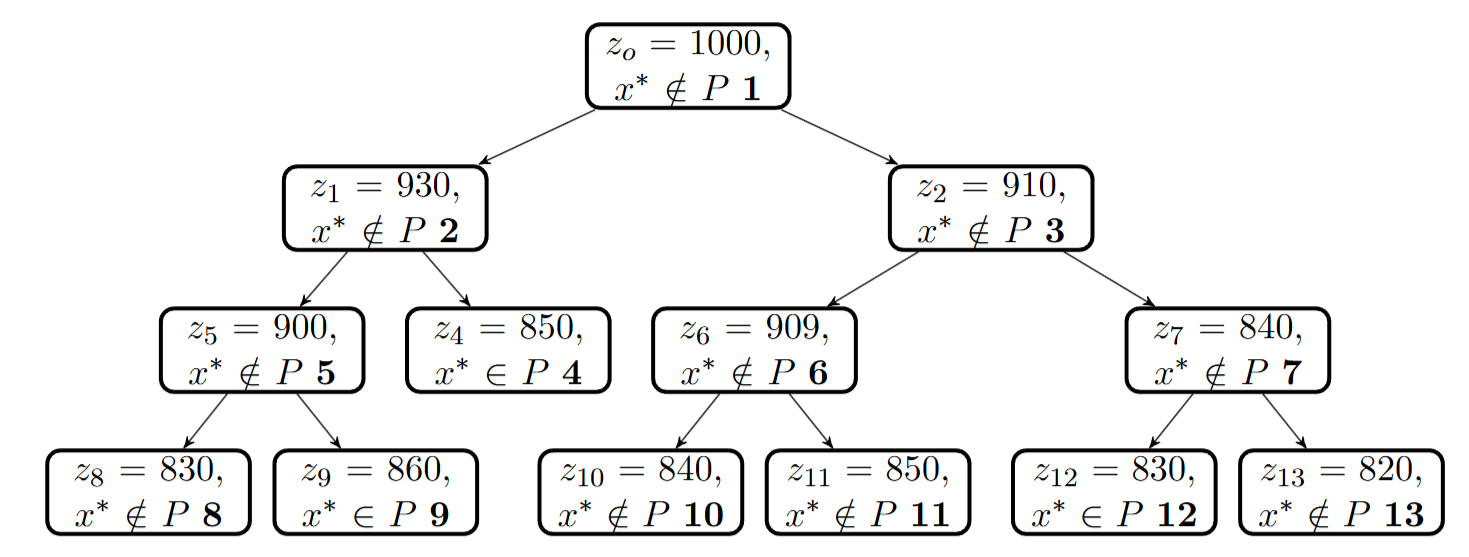
\includegraphics[width=1\linewidth]{img/ejercicios/Capitulo-5/ejercicio_5_1_arbol.png}
    \caption{Árbol de Branch and Bound}
    \label{ex:5:1:fig:arbol}
\end{figure}


\subsubsection{Ejercicio 5.2}
% Fuente: Auxiliar 8, «Métodos de programación entera».
Considere el siguiente problema de programación entera:
\[
\begin{aligned}
\max\quad & x_{1} \;+\; 2\,x_{2} \\[0.5em]
\text{sujeto a}\quad 
& -\,3\,x_{1} \;+\; 4\,x_{2} \;\le 4\\
& 3\,x_{1} \;+\; 2\,x_{2} \;\le 11\\
& 2\,x_{1} \;-\; x_{2} \;\le 5\\
& x_{1},\,x_{2} \;\ge 0,\quad x_{1},\,x_{2} \in \mathbb{Z}.
\end{aligned}
\]
Usar un gráfico para responder las siguientes preguntas:

\begin{enumerate}
  \item[(a)] ¿Cuál es el costo óptimo de la relajación lineal? ¿Y cuál es el costo óptimo del problema de programación entera?
  \item[(b)] ¿Cuál es la envoltura convexa del conjunto de todas las soluciones enteras factibles?
  \item[(c)] Ilustrar cómo funciona el algoritmo de planos de corte de Gomory. Realizar el primer corte.
  \item[(d)] Resolver el problema mediante \emph{branch \& bound}, resolviendo gráficamente las relajaciones.
  \item[(e)] Suponga que se dualiza la restricción \( -\,3\,x_{1} + 4\,x_{2} \le 4 \). ¿Cuál es el valor óptimo \(Z_{D}\) del dual lagrangeano? ¿Cómo cambia el valor de $Z_D$ si se dualiza la restricción \( 2\,x_{1} - x_{2} \le 5 \)? 
\end{enumerate}


\subsubsection{Ejercicio 5.3}
% Fuente: Auxiliar 10, «Repaso de programación entera — Branch and Bound».
En la figura~\ref{ex:5:3:fig:bnb} se observa el árbol con las iteraciones del algoritmo Branch and Bound para un problema de optimización. Cada nodo representa un subproblema y contiene la información del valor objetivo de ese subproblema y si es que la solución encontrada es entera (E), fraccional (NE) o infactible. Note que la etiqueta del problema $P_3$ no está determinada. Responda las siguientes preguntas:

\begin{enumerate}
    \item Suponga que la solución encontrada en $P_5$ es fraccional (NE) y responda cada caso: ¿Este es un problema de maximización o minimización? ¿Qué nodos ramificaría el algoritmo? ¿Qué cota tiene la función objetivo hasta este punto?
    \item ¿Cómo cambian sus respuestas si la solución del problema $P_5$ fuese entera?
\end{enumerate}

\begin{figure}
    \centering
    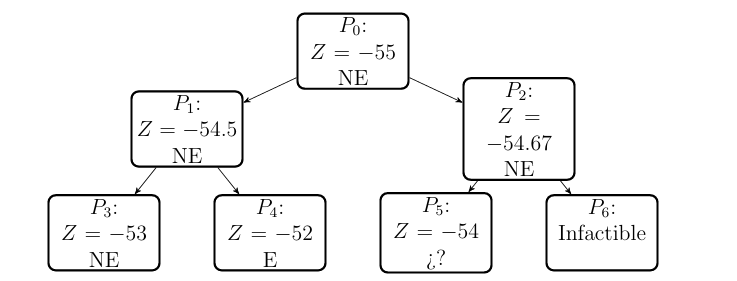
\includegraphics[width=1\linewidth]{img/ejercicios/Capitulo-5/ejercicio_5_3_byb.png}
    \caption{Árbol de Branch and Bound.}
    \label{ex:5:3:fig:bnb}
\end{figure}


\subsubsection{Ejercicio 5.4}
% Fuente: Auxiliar 10, «Repaso de programación entera — Cortes de Gomory».
Considere el siguiente problema de optimización entera:
\[
\begin{aligned}
(P)\quad \min\;& -3x_{1} + 2x_{2}\\
\text{s.a.}\quad
&7x_{1} + 2x_{2} \;\le\; 8,\\
&x_{1} + 2x_{2} \;\le\; 7,\\
&x_{1},\,x_{2}\;\in\;\mathbb{Z}_{\ge0}.
\end{aligned}
\]

\begin{enumerate}
  \item Resuelva gráficamente la relajación lineal de este problema. También muestre la envolvente convexa de los puntos factibles.
  \item Realice una iteración del algoritmo de cortes de Gomory. Discuta gráficamente la optimalidad de la nueva solución encontrada.
\end{enumerate}


\subsubsection{Ejercicio 5.5}
% Fuente: Control 2, Pregunta 1.
El operador de una planta industrial quiere instalar dos tipos de alimentadores
eléctricos para maximizar el número de cargas críticas en hora punta:

\begin{itemize}[nosep]
  \item $x_1$: Alimentadores de distribución tipo A --- energizan $5$ cargas cada uno, demandan $6$\,A de la protección termomagnética principal y ocupan $1$ módulo en el tablero de distribución.
  \item $x_2$: Alimentadores de distribución Tipo B --- energizan $4$ cargas cada uno, demandan $4$\,A de la protección termomagnética principal y ocupan $2$ módulos en el tablero de distribución.
\end{itemize}

La protección termomagnética principal soporta un máximo de $24$\,A y el tablero de distribución solo dispone de $6$ módulos de espacio libre.
 
\begin{enumerate}[label=(\alph*)]
  \item Formule el problema de programación entera. Dibuje la envoltura convexa de las soluciones factibles y encuentre el valor
  óptimo del problema lineal relajado.
  
  \item Proponga un corte o cortes sobre el conjunto factible de modo que el óptimo del problema relajado coincida con el óptimo entero y obtenga el óptimo del problema de forma gráfica.
  
  \textit{No considere (b) para los siguientes incisos}
        
  \item Aplique el primer plano de corte de Gomory sobre el problema original. Muestre y explique cómo afecta al conjunto factible.
  
  \item Resuelva mediante Branch \& Bound (B\&B) usando búsqueda en amplitud. Dibuje el
   árbol de decisiones, indicando en cada nodo la solución de la relajación lineal,
   identifique cada hoja y justifique por qué no se ramifica.
  \item ¿Qué tolerancia de \emph{gap} de optimalidad es necesaria  para que el algoritmo B\&B termine analizando solo $3$ problemas (incluyendo la relajación original), usando búsqueda en amplitud? Analice su respuesta a partir del \textit{trade off} entre un mayor \textit{gap} con una respuesta más precisa.
\end{enumerate}


\subsubsection{Ejercicio 5.6}
% Fuente: Control 2, Pregunta 3, ítems 3–4.
Indique si las siguientes afirmaciones son falsas o verdaderas. En caso de ser verdadera, debe proveer una demostración; en caso contrario, debe dar un contraejemplo.  
\begin{enumerate}
\item Si un programa lineal entero tiene dos soluciones óptimas distintas, entonces tiene infinitas soluciones óptimas. 
\item Sean $P_1$ y $P_2$ las regiones factibles de dos relajaciones de un programa lineal entero de minimización, tales que $P_1 \subseteq P_2$. Si $x^* \in \mathbb{Z}^n$ es una solución óptima del problema entero, con valor óptimo $c^\top x^*$, entonces
$c^\top x^* \geq \min_{x \in P_1} c^\top x \geq \min_{x \in P_2} c^\top x$.
\end{enumerate}


\subsection{Resoluciones}

\subsubsection{Resolución 5.1}
% Fuente: Pauta del Auxiliar 8, «Árbol de Branch and Bound».
Denotemos $z^*$ el incumbente y se entenderá un nodo hoja como uno que no será ramificado (terminal).

\begin{enumerate}
    \item El gap relativo se define como \(\%\text{gap} = \frac{UB - LB}{LB}\), en este caso \(\%\text{gap} = \frac{z^* - LB}{LB}\). De esta forma sí es posible terminar después de explorar 4 nodos, para esto se exploran los nodos \textbf{1, 2, 3} y \textbf{4} y se llega a un \(\%\text{gap} = \frac{930 - 850}{850} = 9.41\% < 10\%\). De esta forma se dejan sin explorar las hojas \textbf{5, 6} y \textbf{7}.
    
    \item No, ya que el incumbente sería al menos 850 (\(z_4 = 850\) y es entero), de esta forma el nodo \textbf{7} no se seguirá ramificando (\(840 = z_7 < z^*\)).
    
    \item Sí, el valor óptimo es \(z = 860\) y se encuentra en el nodo \textbf{9}. Notar que en las demás hojas la función objetivo es menor a este valor.
    
    \item No, de haberse explorado antes el nodo \textbf{4} se tendría \(z^* = 850\), y los nodos \textbf{10, 11, 7} al tener funciones objetivo menores o iguales, efectivamente podrían ser hojas. Sin embargo, no hay manera de que el nodo \textbf{5} sea hoja, ya que no hay solución entera que supere su valor.
    
    \item No, de manera análoga al caso anterior, no hay posibilidad de que los nodos \textbf{2} y \textbf{6} sean hojas.
\end{enumerate}


\subsubsection{Resolución 5.2}
% Fuente: Pauta del Auxiliar 8, «Métodos de programación entera».
\begin{enumerate}
  \item[(a)] Gráficando el conjunto factible se tiene:
  \begin{figure}
      \centering
      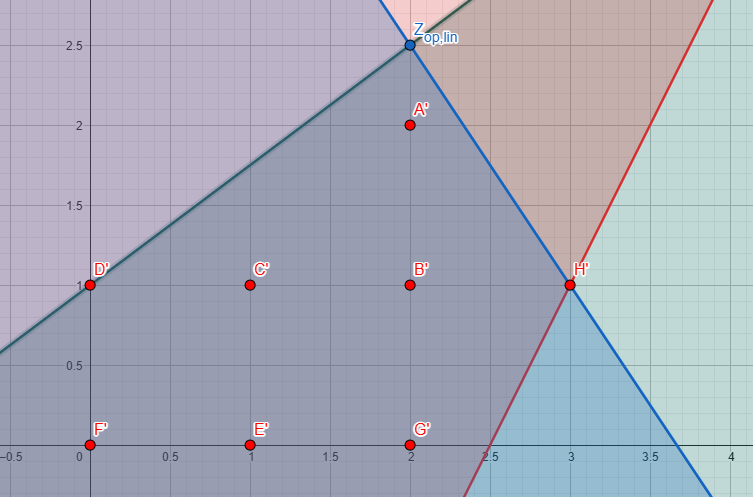
\includegraphics[width=0.7\linewidth]{img/ejercicios/Capitulo-5/ejercicio_5_2_metodos_programacion_entera.png}
      \caption{Conjunto factible Pregunta 3.}
      \label{ex:5:2:fig:conjunto-factible}
  \end{figure}
  La solución de la relajación lineal y del problema original son:
  \[
    z_{\text{LP}} = 7,\quad\text{en }(x_{1},x_{2})=(2,2.5),
    \qquad
    z_{\text{IP}} = 6,\quad\text{en }(x_{1},x_{2})=(2,2).
  \]
  
  \item[(b)] Si se enumeran las soluciones enteras factibles:
  \[
  \{(0,0),(1,0),(2,0),(0,1),(1,1),(2,1),(2,2),(3,1)\}
  \]
  su envoltura convexa es el polígono de vértices
  \[
    \{(0,0),\quad(2,0),\quad(3,1),\quad(2,2),\quad(0,1).\}
  \]
  Es decir,
  \[
    \mathrm{conv}\bigl\{(0,0),(2,0),(3,1),(2,2),(0,1)\bigr\}.
  \]
  Las siguientes rectas producen la envoltura convexa:
  \begin{align*}
      & x_1\geq0\\
      & x_2 \geq 0\\
      & x_2 \geq x_1 -2 \\
      & x_2 \leq 0.5 x_1 +1\\
      & x_2 \leq -x_1 +4
  \end{align*}
  
  \item[(c)] Las matrices del problema relajado en formulación estándar son:
  \[
  A=\begin{pmatrix}
    -3 & 4 &1 & 0 & 0 \\
    3 & 2 & 0 &1&0 \\
    2 & -1&0&0&1
\end{pmatrix}, \quad b= \begin{pmatrix}
    4 \\
    11 \\
    5 
\end{pmatrix}, \quad B=
    \begin{pmatrix}
        -3 & 4 &0  \\
        3 & 2 & 0  \\
        2 & -1&1
    \end{pmatrix}
  \]
  El óptimo de la relajación lineal es $(2,2.5,0,0,5.3)$, luego se realiza el corte sobre $x_2$:
  \begin{equation}
      x_2 + \lfloor\overline{a_{23}}\rfloor \cdot s_1+\lfloor\overline{a_{24}}\rfloor \cdot s_2 \leq \lfloor\overline{a_{20}}\rfloor
  \end{equation}
  donde:
  \begin{align}
     & \overline{a_{23}}=\left(B^{-1}\begin{pmatrix}
          1  \\ 0 \\ 0
      \end{pmatrix} \right)_2 =\frac{1}{6} \\
    & \overline{a_{23}}=\left(B^{-1}\begin{pmatrix}
          0  \\ 1 \\ 0
    \end{pmatrix} \right)_2 =\frac{1}{6} \\
    & \overline{a_{23}}=\left(B^{-1}b \right)_2 =2.5
  \end{align}
De modo que el nuevo corte es:
\begin{equation}
    x_2 \leq 2
\end{equation}
  
  \item[(d)] Comenzamos con $L=-\infty$, donde L corresponde a la mejor corta inferior al ser un problema de maximización.
  
  El nodo raíz corresponde a resolver la relajación lineal del problema original, luego $(x_1, x_2)=(2,2.5)$, donde $z=7$. Dado que no tiene solución entera, se selecciona $x_2$ para particionar el conjunto factible. No se actualiza la cota ($L=-\infty$).

  Los subproblemas generados son:

\begin{equation}
\begin{aligned}
(P2)\quad \min\;& -x_1 \;-\; 2x_2 \\
\text{s.a.}\;& -3x_{1} + 4x_{2} \le 4,\\
& 3x_{1} + 2x_{2} \le 11,\\
& 2x_{1} - x_{2} \le 5,\\
& x_{2} \le 2,\\
& x_{i} \ge 0,\quad i\in\{1,2\}.
\end{aligned}
\end{equation}

\begin{equation}
\begin{aligned}
(P3)\quad \min\;& -x_1 \;-\; 2x_2 \\
\text{s.a.}\;& -3x_{1} + 4x_{2} \le 4,\\
& 3x_{1} + 2x_{2} \le 11,\\
& 2x_{1} - x_{2} \le 5,\\
& x_{2} \ge 3,\\
& x_{i} \ge 0,\quad i\in\{1,2\}.
\end{aligned}
\end{equation}

Dado que el problema $(P3)$ es infactible, se descarta. El problema $(P2)$ alcanza el óptimo en:
\begin{equation}
    x=\left(\frac{7}{3},2\right), \quad z= \frac{19}{3}
\end{equation}
    
Como la solución es no entera, se elige $x_1$ para particionar el conjunto. Aún no hay solución entera, por lo que $L=-\infty$.

Los subproblemas generados a partir de $(P2)$ son:

\begin{equation}
\begin{aligned}
(P4)\quad \min\;& -x_1 \;-\; 2x_2\\
\text{s.a.}\;& -3x_{1} + 4x_{2} \le 4,\\
& 3x_{1} + 2x_{2} \le 11,\\
& 2x_{1} - x_{2} \le 5,\\
& x_{2} \le 2,\\
& x_{1} \le 2,\\
& x_{i} \ge 0,\quad i\in\{1,2\}.
\end{aligned}
\end{equation}

\begin{equation*}
\begin{aligned}
(P5)\quad \min\;& -x_1 \;-\; 2x_2\\
\text{s.a.}\;& -3x_{1} + 4x_{2} \le 4,\\
& 3x_{1} + 2x_{2} \le 11,\\
& 2x_{1} - x_{2} \le 5,\\
& x_{2} \le 2,\\
& x_{1} \ge 3,\\
& x_{i} \ge 0,\quad i\in\{1,2\}.
\end{aligned}
\end{equation*}

La solución de $(P4)$ es:
\begin{equation}
    x=(2,2), \quad z=6
\end{equation}
 Como la solución es entera, se actualiza la cota $L=6$.

 La solución de $(P5)$ es:
 \begin{equation}
     x=(3,1), \quad z= 5
 \end{equation}
 Dado que $z\le L$, se descarta $(P5)$ y la cota superior se mantiene en $L=6$.

 Finalmente, tras explorar todos los nodos, la mejor solución entera es:
 \begin{equation}
    x=(2,2), \quad z=6
\end{equation}
la cual corresponde a la solución del problema original.
  
  \item[(e)] Dado que se está maximizando, se obtendrán cotas superiores. Al relajar dicha restricción con multiplicador \(p\ge0\), el lagrangiano queda:
    \[
      Z(p)
      = \max_{x_{1},x_{2}}
      \Bigl\{\,x_{1} + 2x_{2}
      \;+\; p\,(4 + 3x_{1} - 4x_{2})\Bigr\}
      \quad\text{s.a.}\quad
      \begin{cases}
        3\,x_{1} + 2\,x_{2} \;\le\; 11,\\
        2\,x_{1} - x_{2} \;\le\; 5,\\
        x_{1},x_{2}\ge0,\;x_{1},x_{2}\in\mathbb{Z}.
      \end{cases}
    \]
    Los puntos factibles \((x_{1},x_{2})\) (ignorando la restricción dualizada) generan las siguientes funciones candidatas
    \(\displaystyle\overline{Z}(p)=x_{1}+2x_{2}+p\,(4+3x_{1}-4x_{2})\):

    \[
      \begin{array}{cc|c}
        \hline
        x_{1} & x_{2} & \overline{Z}(p) \\ \hline
        0 & 0 & 4\,p              \\
        0 & 1 & 2                  \\
        0 & 2 & 4 - 4\,p          \\
        0 & 3 & 6 - 8\,p          \\
        0 & 4 & 8 -12\,p          \\
        0 & 5 & 10-16\,p          \\[4pt]
        1 & 0 & 1 + 7\,p          \\
        1 & 1 & 3 + 3\,p          \\
        1 & 2 & 5 -   p          \\
        1 & 3 & 7 - 5\,p          \\
        1 & 4 & 9 - 9\,p          \\[4pt]
        2 & 0 & 2 +10\,p          \\
        2 & 1 & 4 + 6\,p          \\
        2 & 2 & 6 + 2\,p          \\[4pt]
        3 & 1 & 5 + 9\,p          \\
        \hline
      \end{array}
    \]

    A partir de aquí se toma el envolvente superior de estas rectas para obtener
    \(\;Z(p)=\max_{i,j}\overline{Z}(p)\;\) y luego
    \(\displaystyle Z_{D}=\min_{p\ge0}Z(p)\).

Tomando las funciones candidatas \(\overline{Z}(p)=x_{1}+2x_{2}+p(4+3x_{1}-4x_{2})\)
    en cada punto factible y construyendo el envolvente superior, resulta:
    \[
      Z(p)
      = \max_{(i,j)}\overline{Z}(p)
      = 
      \begin{cases}
        10 - 16\,p, & 0 \le p \le \tfrac17,\\[0.3em]
        9 - 9\,p,   & \tfrac17 \le p \le \tfrac29,\\[0.3em]
        5 + 9\,p,   & \tfrac29 \le p \le 3,\\[0.3em]
        2 +10\,p,   & p \ge 3.
      \end{cases}
    \]
    La mejor cota dual se halla en la intersección de la recta $9+9p$ y $5+9p$:
    \[
      \min_{p\ge0}Z(p)
      \;\Longrightarrow\;
      p^* = \tfrac29,
      \quad Z_{D} = Z\bigl(\tfrac29\bigr) = 7.
    \]

Ahora, al relajar la restricción
    \[
      2x_{1} - x_{2} \le 5
    \]
    con lagrangiano
    \[
      Z(q)
      = \max_{x_{1},x_{2}}
      \Bigl\{\,x_{1} + 2x_{2}
      \;+\; q\,(5 - 2x_{1} + x_{2})\Bigr\}
      \quad\text{s.a.}\quad
      \begin{cases}
        -3x_{1} + 4x_{2} \;\le\; 4,\\
        3x_{1} + 2x_{2} \;\le\; 11,\\
        x_{1},x_{2}\ge0,\;x_{1},x_{2}\in\mathbb{Z}.
      \end{cases}
    \]

    Los puntos factibles \((x_{1},x_{2})\) (ignorando la restricción dualizada) generan las siguientes funciones candidatas:

    \[
      \begin{array}{cc|c}
      \hline
      x_{1} & x_{2} & \overline{Z}(q) \\ \hline
      0 & 0 & 0 + 5q \\
      0 & 1 &  2 + 6q \\
      1 & 0 & 1 + 3q \\
      1 & 1 & 3 + 4q \\
      2 & 0 & 2 + 1q \\
      2 & 1 & 4 + 2q \\
      2 & 2 & 6 + 3q \\
      3 & 0 & 3 - 1q \\
      3 & 1 & 5 + 0q \\ \hline
      \end{array}
    \]

    El valor dual es el envolvente superior de estas rectas:
    \[
      Z(q)
      =
      \begin{cases}
        6 + 3q, & 0 \le q \le \tfrac{4}{3},\\[0.3em]
        2 + 6q, & q \ge \tfrac{4}{3}.
      \end{cases}
    \]
    Como ambas ramas tienen pendiente positiva, el mínimo sobre \(q\ge0\) se logra en
    \[
      q^* = 0,
      \qquad
      Z_{D} = Z(0) = 6.
    \]
\end{enumerate}


\subsubsection{Resolución 5.3}
% Fuente: Pauta del Auxiliar 10, «Repaso de programación entera — Branch and Bound».
\begin{enumerate}
  \item Recordar que al agregar restricciones la solución va empeorando al reducir su región factible. Como en este caso la solución aumenta (es menos negativa), se concluye que se está minimizando. El algoritmo ramificaría los nodos \(P_3\) y \(P_5\) ya que son los únicos que pueden seguir dando una mejor solución. En este caso la cota superior (UB) es el \emph{incumbente} \(=-52\) y la cota inferior viene dada por el nodo \(P_5\) (en el mejor de los casos el óptimo podría ser \(-54\)).
  \item Si la solución de \(P_5\) fuese entera, el algoritmo no sigue ramificando ya que el óptimo se encuentra en ese nodo y ambas cotas coinciden (\(\mathrm{UP} = \mathrm{LB} = -54\)).
\end{enumerate}


\subsubsection{Resolución 5.4}
% Fuente: Pauta del Auxiliar 10, «Repaso de programación entera — Cortes de Gomory».
{\color{MidnightBlue}
\begin{enumerate}
  \item
\begin{figure}
    \centering
    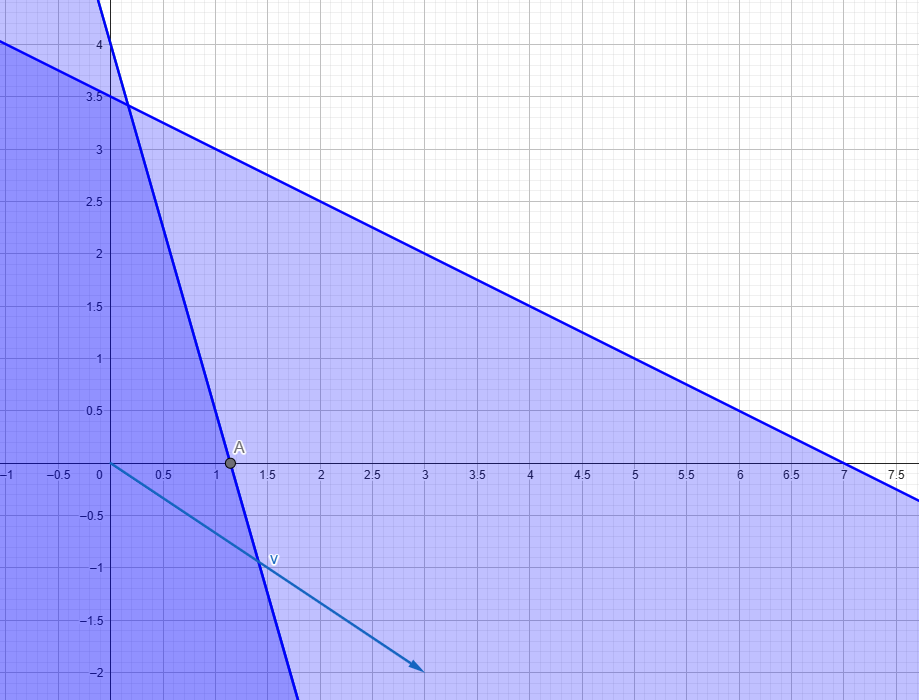
\includegraphics[width=0.8\linewidth]{img/ejercicios/Capitulo-5/ejercicio_5_4_solucion_gomory.png}
    \caption{Solución relajación lineal}
    \label{ex:5:4:fig:relajacion}
\end{figure}
    
El óptimo de la relajación se obtiene en
\[
(x_{1}^{*},x_{2}^{*}) = \Bigl(\tfrac{8}{7},0\Bigr),
\qquad
z^{*} = -3\cdot\tfrac{8}{7} + 2\cdot 0 = -\tfrac{24}{7}.
\]

Los puntos enteros factibles son:
\[
\{(0,0),(0,1),(0,2),(0,3),(1,0)\}.
\]

La envolvente convexa tiene vértices
\((0,0),(1,0),(0,3)\) y viene dada por
\[
x_{1}\ge0,\quad x_{2}\ge0,\quad 3x_{1}+x_{2}\le3.
\]

\begin{figure}
    \centering
    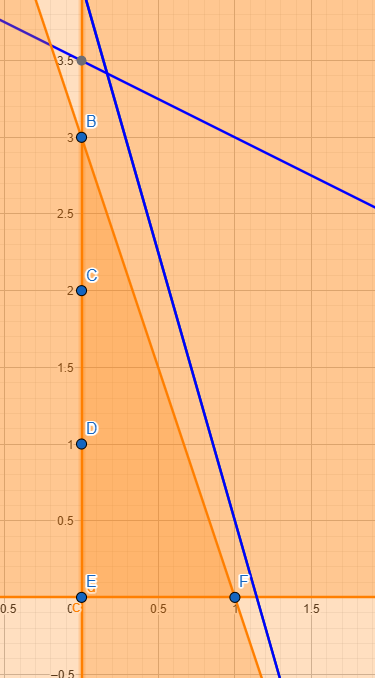
\includegraphics[width=0.5\linewidth]{img/ejercicios/Capitulo-5/ejercicio_5_4_envoltura_convexa.png}
    \caption{Envolvente convexa}
    \label{ex:5:4:fig:envoltura}
\end{figure}
  \item
Las matrices del problema relajado en formulación estándar son:
\[
A=\begin{pmatrix*}
7 & 2 & 1 & 0\\
1 & 2 & 0 & 1
\end{pmatrix*},\qquad
b=\begin{pmatrix}
8\\[0.3em]
7
\end{pmatrix},\qquad
B=\begin{pmatrix}
7 & 0\\
1 & 1
\end{pmatrix}
\]
El óptimo de la relajación lineal es
\[
(x_{1},x_{2},s_{1},s_{2})
=\Bigl(\tfrac{8}{7},\;0,\;0,\;\tfrac{41}{7}\Bigr),
\]
luego se realiza el corte sobre \(x_{1}\):
\begin{equation*}
x_{1}
\;+\;\bigl\lfloor\overline{a}_{12}\bigr\rfloor\,x_{2}
\;+\;\bigl\lfloor\overline{a}_{13}\bigr\rfloor\,s_{1}
\;\le\;\bigl\lfloor\overline{a}_{10}\bigr\rfloor
\end{equation*}
donde
\begin{align*}
\overline{a}_{12}
&=\Bigl(B^{-1}\begin{pmatrix}2\\2\end{pmatrix}\Bigr)_{1}
=\frac{2}{7},\\
\overline{a}_{13}
&=\Bigl(B^{-1}\begin{pmatrix}1\\0\end{pmatrix}\Bigr)_{1}
=\frac{1}{7},\\
\overline{a}_{10}
&=\Bigl(B^{-1}b\Bigr)_{1}
=\frac{8}{7}.
\end{align*}
De modo que el nuevo corte es:
\begin{equation*}
x_{1}\;\le\;1.
\end{equation*}
Añadiendo \(x_{1}\le1\) a la relajación original, el nuevo óptimo es
\[
(x_{1},x_{2}) = (1,0),\qquad z = -3,
\]
que ya es entero y coincide con la solución óptima del programa entero. 
\end{enumerate}
}


\subsubsection{Resolución 5.5}
% Fuente: Pauta del Control 2, Pregunta 1.
\begin{enumerate}
  \item[(a)]
 
\[
\max\; z = 5x_1+4x_2 \qquad
\text{s.a.}\quad
\begin{cases}
6x_1+4x_2 \le 24 & \text{(protecciones)}\\
x_1+2x_2 \le 6 & \text{(tablero)}\\
x_1,x_2 \ge 0,\ \text{enteros.}
\end{cases}
\]
 
\textbf{Relajaci\'on lineal.} Quitando la integralidad, los v\'ertices de la regi\'on factible son
\begin{equation}
    (0,0),\:(4,0),\:(0,3)
\end{equation}
y la intersecci\'on de ambas restricciones. Resolviendo
$6x_1+4x_2=24$ con $x_1+2x_2=6$ se obtiene $x_2=\tfrac32,\ x_1=3$. Evaluando $z$:
\[
(4,0)\to 20,\quad (0,3)\to 12,\quad \Big(3,\tfrac32\Big)\to 21.
\]
El \'optimo de la relajaci\'on es $\big(3,\tfrac32\big)$ con $\boxed{z^*_{LP}=21}$ (fraccionario en $x_2$).
 
\textbf{Envoltura convexa.} El cierre convexo de los puntos enteros factibles tiene v\'ertices
$(0,0),(4,0),(2,2),(0,3)$, basta con añadir la recta $x_1+x_2\le 4$:

\begin{center}
\begin{tikzpicture}[scale=1.35]
  \fill[gray!16]  (0,0) -- (4,0) -- (3,1.5) -- (0,3) -- cycle;
  \fill[blue!14]  (0,0) -- (4,0) -- (2,2)   -- (0,3) -- cycle;
  \draw[step=1,gray!30,very thin] (0,0) grid (4.5,3.5);
  \draw[->] (0,0) -- (4.9,0) node[right]{$x_1$};
  \draw[->] (0,0) -- (0,3.8) node[above]{$x_2$};
  \foreach \x in {1,2,3,4} \draw (\x,0.04)--(\x,-0.04) node[below]{\footnotesize\x};
  \foreach \y in {1,2,3} \draw (0.04,\y)--(-0.04,\y) node[left]{\footnotesize\y};
  % restricciones
  \draw[orange!75!black,thick] (4,0) -- (1.667,3.5) node[pos=0.85,left]{\footnotesize $6x_1{+}4x_2\le24$};
  \draw[teal!70!black,thick]   (0,3) -- (4.5,0.75) node[pos=0.92,below]{\footnotesize $x_1{+}2x_2\le6$};
  % faceta entera
  \draw[blue!70!black,very thick] (4,0) -- (2,2) node[midway,below left,blue!60!black]{\footnotesize $x_1{+}x_2\le4$};
  % puntos enteros
  \foreach \p in {(0,0),(1,0),(2,0),(3,0),(4,0),(0,1),(1,1),(2,1),(3,1),(0,2),(1,2),(2,2),(0,3)}
    \fill \p circle (1.5pt);
  % optimo relajacion
  \draw[red!75!black,thick] (3,1.5) circle (3.2pt);
  \node[red!70!black,above right,inner sep=1pt] at (3,1.5) {\footnotesize $(3,\tfrac32)$, $z{=}21$};
  % optimo entero
  \fill[green!55!black] (4,0) circle[radius=2.2pt];
  \node[green!45!black,above right,inner sep=1pt] at (4,0.05) {\footnotesize $(4,0)$, $z{=}20$};
\end{tikzpicture}
\end{center}
 
  \item[(b)]
 
Basta a\~nadir la recta añadida en la envoltura convexa
\[
\boxed{x_1+x_2 \le 4.}
\]
Con ella, la regi\'on de la relajaci\'on pasa a ser exactamente $\operatorname{conv}$, con v\'ertices
\begin{equation*}
    (0,0),\:(4,0),\:(2,2),\:(0,3) \: \implies \:\textit{todos enteros}
\end{equation*}
. La restricci\'on de potencia
$6x_1+4x_2\le24$ queda redundante (solo toca en $(4,0)$). Optimizando $z=5x_1+4x_2$:
\[
(4,0)\to 20,\quad (2,2)\to 18,\quad (0,3)\to 12 \;\Rightarrow\; \text{\'optimo LP en }(4,0),\ z=20,
\]
que coincide con el \'optimo entero. Es el corte ``ideal'': uno solo basta para obtener la solución óptima entera resolviendo el problema relajado.
 
  \item[(c)]

Aplicando el corte de Gomory sobre la fila asociada a \(x_2\),
\[
x_{B_r}+
\sum_{j\in N}
\left\lfloor (B^{-1}A_j)_r\right\rfloor x_j
\leq
\left\lfloor (B^{-1}b)_r\right\rfloor,
\qquad r=2,
\]
resulta
\[
x_2+
\left\lfloor-\frac18\right\rfloor s_1+
\left\lfloor\frac34\right\rfloor s_2
\leq
\left\lfloor\frac32\right\rfloor.
\]

Por tanto,
\[
x_2-s_1\leq 1.
\]

Usando
\[
s_1=24-6x_1-4x_2,
\]
se obtiene
\[
x_2-\left(24-6x_1-4x_2\right)\leq 1,
\]
y finalmente
\[
\boxed{6x_1+5x_2\leq 25.}
\]
 
\textbf{Verificaci\'on.} En $\big(3,\tfrac32\big)$ da $25{,}5>25$ (elimina el v\'ertice fraccionario);
en todo punto entero factible se cumple $\le 25$ (no se pierde ninguna soluci\'on entera). El nuevo
\'optimo de la relajaci\'on pasa a $\big(\tfrac{10}{3},1\big)$, $z=\tfrac{62}{3}\approx 20{,}67$
(todav\'ia fraccionario: har\'ian falta m\'as cortes).

\begin{center}
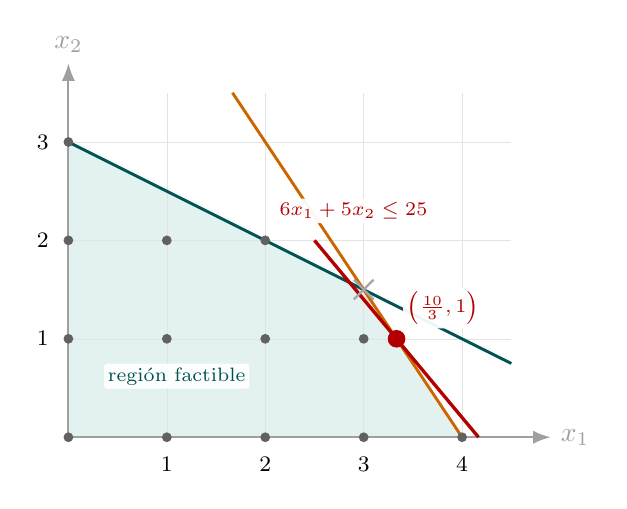
\begin{tikzpicture}[
  scale=1.25,
  >=Latex,
  axis/.style={->,line width=.75pt,gray!75},
  cA/.style={orange!80!black,line width=1.05pt},
  cB/.style={teal!65!black,line width=1.05pt},
  cNew/.style={red!70!black,line width=1.2pt},
  dot/.style={circle,fill=black!62,inner sep=1.25pt},
  tag/.style={
    font=\scriptsize,
    fill=white,
    fill opacity=.94,
    text opacity=1,
    inner sep=1.4pt,
    rounded corners=1pt
  }
]

  % Puntos geométricos relevantes
  \coordinate (O) at (0,0);
  \coordinate (B) at (4,0);
  \coordinate (C) at (3,1.5);              % óptimo anterior
  \coordinate (D) at (0,3);
  \coordinate (P) at ({10/3},1);           % nuevo óptimo
  \coordinate (Q) at ({20/7},{11/7});      % intersección rojo--verde

  % Región factible final
  \fill[teal!11] (O) -- (B) -- (P) -- (Q) -- (D) -- cycle;

  % Parte de la región anterior eliminada por la nueva restricción
  \fill[red!13] (C) -- (P) -- (Q) -- cycle;

  % Cuadrícula
  \draw[step=1,gray!22,very thin] (0,0) grid (4.5,3.5);

  % Ejes
  \draw[axis] (0,0) -- (4.9,0) node[right] {$x_1$};
  \draw[axis] (0,0) -- (0,3.8) node[above] {$x_2$};

  % Marcas de los ejes
  \foreach \x in {1,2,3,4}
    \draw (\x,.045) -- (\x,-.045)
      node[below=2pt,font=\footnotesize] {\x};

  \foreach \y in {1,2,3}
    \draw (.045,\y) -- (-.045,\y)
      node[left=2pt,font=\footnotesize] {\y};

  % Restricciones originales
  \draw[cA] (4,0) -- ({5/3},3.5);
  \draw[cB] (0,3) -- (4.5,.75);

  % Nueva restricción: 6x_1 + 5x_2 <= 25
  \draw[cNew] ({25/6},0) -- (2.5,2);

  % Puntos enteros factibles
  \foreach \x/\y in {
    0/0,1/0,2/0,3/0,4/0,
    0/1,1/1,2/1,3/1,
    0/2,1/2,2/2,
    0/3
  }
    \node[dot] at (\x,\y) {};

  % Óptimo anterior, marcado de forma discreta
  \draw[gray!70,line width=.85pt]
    ($(C)+(-.10,-.10)$) -- ($(C)+(.10,.10)$);
  \draw[gray!70,line width=.85pt]
    ($(C)+(-.10,.10)$) -- ($(C)+(.10,-.10)$);

  % Nuevo óptimo
  \fill[red!70!black] (P) circle[radius=2.55pt];
  \node[tag,text=red!70!black,anchor=south west]
    at ($(P)+(.06,.10)$)
    {$\left(\frac{10}{3},1\right)$};

  % Etiquetas limpias, fuera de las intersecciones
  \node[tag,text=teal!65!black] at (1.10,.62)
    {\scriptsize región factible};

  \node[tag,text=red!70!black,anchor=west] at (2.10,2.30)
    {$6x_1+5x_2\le 25$};

\end{tikzpicture}
\end{center}

 
 
  \item[(d)]
 
Ra\'iz: relajaci\'on $\big(3,\tfrac32\big)$, $z=21$. Se ramifica sobre la variable fraccionaria $x_2$.
La b\'usqueda en amplitud procesa por niveles: ra\'iz $\to\{x_2\le1,\ x_2\ge2\}\to\{x_1\le3,\ x_1\ge4\}$.
 
\begin{center}
\begin{tikzpicture}[
  box/.style={draw,rounded corners,align=center,minimum width=2.9cm,minimum height=1.05cm,
              font=\footnotesize,inner sep=2pt},
  opt/.style={box,very thick,fill=green!12},
  leaf/.style={box,fill=blue!6},
  edgelbl/.style={font=\scriptsize,fill=white,inner sep=1pt}
]
  \node[box]  (root) at (0,0)   {$(3,\tfrac32)$\\ $z=21$ (fracc.)};
  \node[box]  (n1)   at (-3,-2) {$(\tfrac{10}{3},1)$\\ $z\approx20{,}7$ (fracc.)};
  \node[leaf] (n2)   at (3,-2)  {$(2,2)$\\ $z=18$ (hoja)};
  \node[leaf] (n11)  at (-5,-4) {$(3,1)$\\ $z=19$ (hoja)};
  \node[opt]  (n12)  at (-1,-4) {$(4,0)$\\ $z=20$ ($\bigstar$ \'optimo)};
  \draw[->] (root) -- (n1)  node[edgelbl,pos=0.5]{$x_2\le1$};
  \draw[->] (root) -- (n2)  node[edgelbl,pos=0.5]{$x_2\ge2$};
  \draw[->] (n1)   -- (n11) node[edgelbl,pos=0.5]{$x_1\le3$};
  \draw[->] (n1)   -- (n12) node[edgelbl,pos=0.5]{$x_1\ge4$};
\end{tikzpicture}
\end{center}
 
\noindent\textbf{Recorrido.}
\begin{itemize}[nosep]
  \item $x_2\le1$: LP $\to\big(\tfrac{10}{3},1\big)$, $z\approx20{,}7$; fraccionaria en $x_1\Rightarrow$ se ramifica.
  \item $x_2\le1,\ x_1\le3$: LP $\to(3,1)$, $z=19$; \textbf{hoja} (entera). Incumbente provisional.
  \item $x_2\le1,\ x_1\ge4$: LP $\to(4,0)$, $z=20$; \textbf{hoja} (entera). Mejora el incumbente.
  \item $x_2\ge2$: LP $\to(2,2)$, $z=18$; \textbf{hoja} (entera), dominada por $(4,0)$.
\end{itemize}
 
\noindent Cada hoja se cierra porque su relajaci\'on ya es entera (criterio de integralidad), as\'i que
no queda nada que ramificar. El \'optimo entero es $\boxed{(x_1,x_2)=(4,0),\ z^*=20}$: instalar
$4$ m\'odulos PV y $0$ bater\'ias, abasteciendo $20$ viviendas.
 
  \item[(e)]
 
Con b\'usqueda en amplitud, los tres problemas resueltos son la \textbf{ra\'iz}, el nodo
\textbf{$x_2\le1$} y el nodo \textbf{$x_2\ge2$}. Al terminar de procesarlos:
\begin{itemize}[nosep]
  \item Incumbente (mejor entera): $(2,2)$, $\;z_{LB}=18$.
  \item Mejor cota superior de los nodos pendientes (los hijos de $x_2\le1$, a\'un sin resolver,
        que heredan la cota de su padre): $z_{UB}=\tfrac{62}{3}\approx 20{,}67$.
\end{itemize}
El gap en ese punto es
\[
\text{gap}_{\text{abs}} = z_{UB}-z_{LB} = \tfrac{62}{3}-18 = \tfrac{8}{3}\approx 2{,}67.
\]
Para que el algoritmo se detenga \emph{sin} resolver esos hijos, la tolerancia debe cumplir
\[
\boxed{\varepsilon_{\text{abs}} \ge \tfrac{8}{3}\approx 2{,}67}
\qquad\Longleftrightarrow\qquad
\varepsilon_{\text{rel}} \ge \frac{8/3}{18} = \frac{4}{27}\approx 14{,}8\%
\ \ \text{(respecto al incumbente),}
\]
o bien $\dfrac{8/3}{62/3}=\dfrac{4}{31}\approx 12{,}9\%$ respecto a la cota. Con esa tolerancia, B\&B
devuelve $(2,2)$ con $z=18$, garantizado a lo sumo $\tfrac{8}{3}$ por debajo del \'optimo (el \'optimo
real es $20$; el error real es $2$). Es el clásico compromiso entre tolerancia y esfuerzo: un gap m\'as
holgado detiene antes la b\'usqueda pero entrega una soluci\'on sub\'optima.
\end{enumerate}


\subsubsection{Resolución 5.6}
% Fuente: Pauta del Control 2, Pregunta 3, ítems 3–4.
{\color{MidnightBlue}
\begin{enumerate}
    \item \textbf{Falsa.} En un programa lineal \emph{entero}, el segmento entre dos soluciones enteras factibles no tiene por qué estar compuesto por puntos enteros.

    Por ejemplo, considérese
    \[
        \min \; 0
    \]
    sujeto a
    \[
        0\leq x\leq 1,
        \qquad x\in\mathbb{Z}.
    \]
    Las únicas soluciones factibles son $x=0$ y $x=1$. Ambas son óptimas, pues la función objetivo vale $0$ en ambas, pero no existen infinitas soluciones óptimas enteras. Por tanto, la afirmación es falsa.

    \item \textbf{Verdadera.} Sea $X_I$ la región factible del programa lineal entero. Como $P_1$ y $P_2$ son relajaciones del problema entero, se cumple
    \[
        X_I\subseteq P_1,
        \qquad
        X_I\subseteq P_2.
    \]
    En particular, como $x^*\in X_I$, entonces $x^*\in P_1$. Por consiguiente,
    \[
        c^\top x^*\geq \min_{x\in P_1} c^\top x.
    \]
    Además, dado que $P_1\subseteq P_2$, al minimizar sobre un conjunto más grande el valor óptimo no puede aumentar; así,
    \[
        \min_{x\in P_1}c^\top x
        \geq
        \min_{x\in P_2}c^\top x.
    \]
    Por tanto,
    \[
        c^\top x^*
        \geq
        \min_{x\in P_1}c^\top x
        \geq
        \min_{x\in P_2}c^\top x.
    \]
\end{enumerate}
}


\newpage
\section{Optimización continua y convexidad}

\subsection{Convexidad}

\subsubsection{Conjuntos convexos.}

\subsubsection{Funciones convexas y estrictamente convexas.}

\subsubsection{Propiedades de los problemas convexos.}

\subsection{Optimización con restricciones.}

\subsubsection{Condiciones de Karush–Kuhn–Tucker.}

\subsection{Optimización sin restricciones.}

\subsubsection{Gradiente y Hessiano.}

\subsection{Condiciones de optimalidad sin restricciones.}

\subsection{Lagrangiano.}

\subsection{Ejercicios}

\subsubsection{Ejercicio 6.1}
% Fuente: Auxiliar 3, «Convexidad — Función convexa».
\begin{enumerate}
    \item Sea \( g : \mathbb{R}^n \rightarrow \mathbb{R} \) una función convexa. Se define 
\[
f(x) = e^{g(x)}.
\]
Muestre que \( f \) es convexa. Hint: La función exponencial es convexa.
\item Sea 
\[
f_r(x) = f(Ax + D b),
\]
donde \( f : \mathbb{R}^n \rightarrow \mathbb{R} \) es una función convexa, \( A \) es una matriz de \( m \times n \), y \( b \) es un vector en \( \mathbb{R}^n \). Muestre que $f_r$ es convexa.
\end{enumerate}


\subsubsection{Ejercicio 6.2}
% Fuente: Auxiliar 3, «Convexidad — Soluciones de una inecuación cuadrática».
\begin{itemize}
    \item[(a)] \textbf{(Teorema)} 
Demuestre que un conjunto es convexo si y solo si su intersección con una línea arbitraria 
\[
\{ \hat{x} + t v \mid t \in \mathbb{R} \}
\]
es convexa.
    \item[(b)] Sea \( C \subseteq \mathbb{R}^n \) el conjunto solución de una desigualdad cuadrática:

\[
C = \left\{ x \in \mathbb{R}^n \;\middle|\; x^T A x + b^T x + c \leq 0 \right\},
\]

donde \( A \in \mathbb{S}^n \), \( b \in \mathbb{R}^n \), y \( c \in \mathbb{R} \).

Muestre que \( C \) es convexo si \( A \succeq 0 \).
    
    \textbf{HINT}: \[
\text{Una matriz } A \in \mathbb{R}^{n \times n} \text{ es semidefinida positiva si y solo si:}
\]
\[
v^T A v \geq 0 \quad \text{para todo } v \in \mathbb{R}^n.
\]
\end{itemize}


\subsubsection{Ejercicio 6.3}
% Fuente: Auxiliar 10, «Conceptual».
Justifique su respuesta. Si la afirmación es falsa, entregue un contraejemplo.
\begin{enumerate}
    \item Si un punto $x^*$ cumple las condiciones necesarias de primer orden, entonces $x^*$ puede no ser un óptimo local.
    \item En un problema de optimización no convexo, todo mínimo local es también un mínimo global.
    \item Un problema de optimización no lineal convexo y acotado\footnote{Un problema es acotado inferiormente si su función objetivo no puede tomar valores arbitrariamente pequeños dentro del conjunto factible.}, siempre admite una solución óptima.
    \item Si un punto cumple con las condiciones de KKT para un problema no lineal, entonces necesariamente es una solución óptima.
\end{enumerate}


\subsubsection{Ejercicio 6.4}
% Fuente: Auxiliar 10, «KKT — Pregunta 1».
Resolver el siguiente problema para cada valor posible de $A$ utilizando KKT. Verifique que las condiciones de KKT son suficientes para asegurar la optimalidad del problema primal y dual.

\[
\begin{aligned}
\min \quad & J = x_1^2 + x_2^2 + x_3^2 + x_4^2 \\
\text{s.a.} \quad & x_1 + x_2 + x_3 + x_4 = 1 \\
& x_4 \leq A
\end{aligned}
\]


\subsubsection{Ejercicio 6.5}
% Fuente: Auxiliar 10, «KKT — Pregunta 2».
Un lago recibe descargas industriales contaminantes $u_i$ en $n$ puntos $i = 1, \dots, N$ ($u_i$ es la demanda biológica por oxígeno y se mide en [mg $O_2$/litro]).

Una reducción de $x_i$ unidades en las emisiones de la planta $i$ conlleva un costo $c_i(x_i) = \beta_i [\exp(\alpha_i x_i) - 1]$ con $\alpha_i, \beta_i$ constantes conocidas y estrictamente positivas. Para alcanzar un nivel aceptable de calidad del agua se debe satisfacer la restricción $\sum_{i=1}^{n} a_i x_i \geq b$, donde $a_i$ representa el impacto que tiene la fuente $i$ sobre el lago y $b \leq \sum_{i=1}^{n} a_i u_i$, lo que nos lleva a considerar el problema:

\[
\text{(P)} \quad \min \sum_{i=1}^{n} \beta_i (e^{\alpha_i x_i} - 1)
\quad \text{s.a.} \quad
\sum_{i=1}^{n} a_i x_i \geq b, \quad
0 \leq x_i \leq u_i \quad \forall i = 1, \dots, n
\]
\begin{enumerate}
  \item[(a)] Discuta la unicidad de las soluciones óptimas.
  \item[(b)] Explicite las condiciones KKT y pruebe que el multiplicador $\mu$ asociado a $\sum_{i=1}^{n} a_i x_i \geq b$ es estrictamente positivo.
  \item[(c)] Muestre que la solución óptima se puede expresar como 
  \[
  x_i = \frac{1}{\alpha_i} \left[ \ln\left( \frac{\mu a_i}{\beta_i \alpha_i} \right) \right]_{0}^{u_i}
  \]
  donde $[z]_0^u$ es la truncación del número $z$ al intervalo $[0, u]$, es decir
  \[
  [z]_0^u =
  \begin{cases}
  0 & \text{si } z < 0 \\
  z & \text{si } 0 \leq z \leq u \\
  u & \text{si } z > u
  \end{cases}
  \]
  \item[(d)] Encuentre una ecuación para $\mu$ y muestre que tiene solución única.
  \item[(e)] Resuelva para el caso en que $u_i = u$ y $\frac{a_i}{\beta_i \alpha_i} = \gamma$ son constantes y calcule los $x_i$ óptimos.
\end{enumerate}


\subsubsection{Ejercicio 6.6}
% Fuente: Control 2, Pregunta 2.
Considere el siguiente problema de optimización no lineal:

\begin{equation*}
\begin{aligned}
    (\bar{P})\quad \min_{x_1,x_2} \quad 
    & \frac{1}{2}k_1x_1^2
    + \frac{1}{2}k_2(x_2-x_1)^2
    + \frac{1}{2}k_3(l-x_2)^2 \\
    \text{s.a.} \quad 
    & \frac{w}{2}-x_1 \leq 0, \qquad (R1) \\
    & w+x_1-x_2 \leq 0, \qquad (R2) \\
    & \frac{w}{2}-l+x_2 \leq 0. \qquad (R3)
\end{aligned}
\end{equation*}

donde $w,l,k_1,k_2,k_3$ son parámetros positivos y se cumple que $l>2w$.

\begin{enumerate}[label=(\alph*)]
    \item Demuestre que $(\bar{P})$ es convexo y encuentre al menos un punto que satisfaga la condición de \textit{Slater}.

    \item Plantee el problema dual lagrangiano. Indique cómo se relaciona el valor óptimo de este problema con el de $(\bar{P})$. 

    \item Plantee las condiciones de KKT para $(\bar{P})$ y justifique por qué es posible encontrar una solución óptima en base a ellas.

    \item Suponga que $w=2$, $l=10$, $k_1=k_2=k_3=1$ y, 
    además, que las variables duales asociadas a las restricciones (R1) y (R2) son cero. Demuestre que el problema tiene solución y determínela.
\end{enumerate}


\subsubsection{Ejercicio 6.7}
% Fuente: Control 2, Pregunta 3, ítems 1–2.
Indique si las siguientes afirmaciones son falsas o verdaderas. En caso de ser verdadera, debe proveer una demostración; en caso contrario, debe dar un contraejemplo.  
\begin{enumerate}
\item Sea $f_1:\mathbb{R}^{n} \rightarrow \mathbb{R}$ y $f_2:\mathbb{R}^{n} \rightarrow \mathbb{R}$ dos funciones convexas. Entonces, se tiene que $g(x)= \max(f_1(x),f_2(x))$ es una función convexa.
\item La función $f(x_1,x_2)=x_1^{2}+5x_2^{2}-2x_1x_2-10x_1+10x_2$ es convexa.
\end{enumerate}


\subsection{Resoluciones}

\subsubsection{Resolución 6.1}
% Fuente: Pauta del Auxiliar 3, «Convexidad — Función convexa».
{\color{MidnightBlue}
\begin{enumerate}
  \item
\begin{align*}
    f(\lambda x + (1-\lambda) y)&=e^{g(\lambda x + (1-\lambda) y)}\\
    & \leq e^{\lambda g(x) + (1-\lambda) g(y)} \quad & \text{por convexidad de g(.)}\\
    & \leq \lambda e^{g(x)}+(1-\lambda)e^{g(y)} & \text{por convexidad de exp(.)}\\
    &= \lambda f(x) + (1-\lambda)f(y)
\end{align*}
  \item
Definiendo $g(x) =A x+Db$. Se puede ver que g(.) corresponde a una transformación lineal:
\begin{align*}
g(\lambda x + (1-\lambda)y)&=\lambda A x + (1-\lambda)A y + Db\\
&=\lambda(Ax+Db)+(1-\lambda)(Ay+Db)\\
&=\lambda g(x)+(1-\lambda)g(y)
\end{align*}

Luego
\begin{align*}
    f_r(\lambda x + (1-\lambda) y)&=f(g(\lambda x + (1-\lambda) y))\\
    & = f(\lambda g(x) + (1-\lambda) g(y)) \quad & \text{por linealidad de g(.)}\\
    & \leq \lambda f(g(x)) +(1-\lambda)f(g(y)) & \text{por convexidad de f(.)}\\
    &= \ \lambda f_r(x) +(1-\lambda)f_r(y)
\end{align*}
\end{enumerate}
}


\subsubsection{Resolución 6.2}
% Fuente: Pauta del Auxiliar 3, «Convexidad — Soluciones de una inecuación cuadrática».
{\color{MidnightBlue}
\begin{itemize}
  \item[(a)]
  \begin{itemize}
  \item[$\Rightarrow$:] Supongamos que $S$ es convexo. Queremos probar que $S\cap L$ es convexo.

  Sea arbitraria la línea 
  $L=\{\hat x+t v\mid t\in\mathbb{R}\}$ y tomemos dos puntos 
  \[
    y_1 = \hat x + t_1 v,\quad 
    y_2 = \hat x + t_2 v
  \]
  en $S\cap L$. Para cualquier $\lambda\in[0,1]$ tenemos
  \[
    \lambda y_1 + (1-\lambda)y_2 
    = \lambda(\hat x + t_1 v) + (1-\lambda)(\hat x + t_2 v)
    = \hat x + (\lambda t_1 + (1-\lambda)t_2)\,v,
  \]
  que pertenece a $L$. Como además $S$ es convexo, $\lambda y_1+(1-\lambda)y_2\in S$.  
  Por lo tanto $\lambda y_1 + (1-\lambda)y_2 \in S\cap L$, y $S\cap L$ es convexo.
  \item[$\Leftarrow$:] Ahora supongamos que para toda línea $L$ la intersección $S\cap L$ es convexa. 
  Queremos probar que $S$ es convexo en $\mathbb{R}^n$. 

  Tomemos dos puntos arbitrarios $x_1,x_2\in S$. Definimos la línea que los contiene:
  \[
    L = \{\,x_1 + t\,(x_2 - x_1)\mid t\in\mathbb{R}\,\}.
  \]
  Como $x_1,x_2\in S\cap L$ y por hipótesis $S\cap L$ es convexo, para todo $\lambda\in[0,1]$ se cumple
  \[
    \lambda x_1 + (1-\lambda)x_2 
    \;\in\; S\cap L
    \;\subseteq\; S.
  \]
  Esto demuestra que $S$ es convexo.
  \end{itemize}
  \item[(b)] Suponga que
    \[
    A\succeq 0.
    \]
    Queremos demostrar que \(C\) es convexo.

    Por el resultado anterior, basta estudiar la intersección de \(C\) con una línea arbitraria. Sea
    \[
    x=\hat{x}+tv,
    \]
    donde \(\hat{x},v\in\mathbb{R}^n\) y \(t\in\mathbb{R}\).

    Reemplazando en la desigualdad cuadrática:
    \[
    (\hat{x}+tv)^\top A(\hat{x}+tv)
    +
    b^\top(\hat{x}+tv)
    +
    c
    \leq 0.
    \]

    Expandiendo:
    \[
    \hat{x}^\top A\hat{x}
    +
    2t v^\top A\hat{x}
    +
    t^2 v^\top A v
    +
    b^\top \hat{x}
    +
    t b^\top v
    +
    c
    \leq 0.
    \]

    Agrupando en términos de \(t\):
    \[
    \phi(t)
    =
    (v^\top A v)t^2
    +
    \left(2v^\top A\hat{x}+b^\top v\right)t
    +
    \hat{x}^\top A\hat{x}
    +
    b^\top \hat{x}
    +
    c
    \leq 0.
    \]

    Como \(A\succeq 0\), se cumple que
    \[
    v^\top A v\geq 0
    \qquad
    \forall v\in\mathbb{R}^n.
    \]
    Por lo tanto, \(\phi(t)\) es una función convexa en \(t\).

    Luego, el conjunto
    \[
    \{t\in\mathbb{R}\mid \phi(t)\leq 0\}
    \]
    es un subnivel \footnote{es un subconjunto de $\mathbb{R}$ formado por todos los valores de t que cumplen la condición $ϕ(t)≤0$} de una función convexa de una variable, y por tanto es convexo.

    Como esto ocurre para toda línea, se concluye que \(C\) es convexo.

    \[
    A\succeq 0 \Rightarrow C\text{ es convexo.}
    \]
\end{itemize}
}


\subsubsection{Resolución 6.3}
% Fuente: Pauta del Auxiliar 10, «Conceptual».
\begin{enumerate}
  \item \textbf{Verdadero.} Las condiciones necesarias de primer orden establecen que si $x^*$ es un mínimo local, entonces $\nabla f(x^*) = 0$. Sin embargo, el recíproco no es cierto: el que $\nabla f(x^*) = 0$ no implica que $x^*$ sea un mínimo local. La condición $\nabla f(x^*) = 0$ sólo garantiza que no hay dirección de descenso en primera orden, pero no da información sobre la curvatura. Si el Hessiano no es positivo semidefinido, el punto puede ser un punto de silla o un máximo. Por tanto, la afirmación es verdadera.
  \item \textbf{Falso}. Se requiere un ejemplo no convexo donde el mínimo no sea global. Una función será no convexa si tiene más de un punto donde el gradiente se anula. Por ejemplo:
    \[
    f(x)=x^2+x^3
    \]
    se tiene que 0 es mínimo, ya que su derivada se anula y a su vez $f''(0)=0$, por lo que es mínimo local. Pero no es global, ya que $f(x)<f(0)$ si $x<1$.
  \item \textbf{Falso}
    El siguiente problema no lineal es acotado:
\[
\min \left\{ \frac{1}{x} \right\} \quad \text{sujeto a } x \geq 1
\]

Notamos que \( f(x) = \frac{1}{x} \) es convexo si:
\[
\lambda \in [0, 1]
\]
\[
f(\lambda x + (1 - \lambda)y) \leq \lambda f(x) + (1 - \lambda)f(y)
\]

Como \( x, y \geq 1 \) basta corroborar que se cumple:
\[
xy \leq (\lambda y + (1 - \lambda)x)(\lambda x + (1 - \lambda)y)
\]

Efectivamente:
\[
(\lambda y + (1 - \lambda)x)(\lambda x + (1 - \lambda)y) = \lambda^2 xy + (\lambda - \lambda^2)x^2 + (1 - \lambda)^2xy + (\lambda - \lambda^2)y^2
\]
\[
= -\lambda^2(x - y)^2 + \lambda(x - y)^2 + xy = \lambda(1 - \lambda)(x - y)^2 + xy \geq xy.
\]

\[
\Rightarrow f(x) \text{ es convexa, pero el mínimo está indeterminado.}
\]
  \item \textbf{Falso} Un ejemplo clásico donde se cumple que el gradiente es cero pero no se tiene un mínimo local, debido a que el problema no es acotado, es el siguiente:
\begin{align*}
\min \quad & -(x - 2)^2 \\
\text{s.a.} \quad & x \geq 1
\end{align*}
Calculamos las condiciones de Karush-Kuhn-Tucker (KKT). Sea $\lambda$ el multiplicador de la restricción \( x \geq 1 \). La condición de estacionaridad es:

\[
\frac{d}{dx} [-(x - 2)^2 + \lambda(1-x)] = 0 \Rightarrow -2(x - 2) - \lambda = 0
\]

La condición de complementariedad:

\[
\lambda(1 - x) = 0
\]

Y las condiciones de factibilidad:

\[
x \geq 1, \quad \lambda \geq 0
\]

Proponemos el punto \( x = 2 \), entonces:

\[
-2(2 - 2) - \lambda = 0 \Rightarrow \lambda = 0
\]
\[
\lambda(1 - x) = 0(1 - 2) = 0
\]
\[
x = 2 \geq 1, \quad \lambda = 0 \geq 0
\]

El punto \( x = 2 \) satisface todas las condiciones KKT, pero no es un mínimo global ni local, ya que la función es estrictamente cóncava (el problema no es convexo) y no está acotado superiormente. En este caso, al aumentar \( x \), la función \( -(x - 2)^2 \) decrece indefinidamente.

\textbf{Observación:} El hecho de que un punto satisfaga las condiciones de KKT no garantiza que sea una solución óptima en un problema no convexo.
\end{enumerate}


\subsubsection{Resolución 6.4}
% Fuente: Pauta del Auxiliar 10, «KKT — Pregunta 1».
Lo primero que corresponde hacer antes de utilizar las condiciones de KKT es verificar que se cumplan las hipótesis que aseguran la \textbf{suficiencia}:

\begin{itemize}
  \item \textbf{Funciones diferenciables:} Tanto la función objetivo (\(J\)) como las funciones que definen las restricciones de igualdad y desigualdad (\(h\) y \(f\)) son diferenciables.

  \item \textbf{Problema convexo:} El problema es convexo pues la función \(J\) es convexa (forma cuadrática con matriz definida positiva)\footnote{También se puede concluir esto si se tiene en cuenta que la operación suma mantiene la convexidad de las funciones y las funciones sumadas son todas convexas.}, la restricción de desigualdad es convexa (es una función afín) y la restricción de igualdad es afín.

  \item \textbf{Condición de Slater:} Se cumple, basta con elegir un punto \(\hat{x}\) que cumpla con \(f(\hat{x}) = \hat{x}_4 - A < 0\) y que satisfaga la restricción de igualdad. El punto \(\hat{x}(x_4) = (-x_4+1,\, 0,\, 0,\, x_4)\) siempre satisface la restricción de igualdad y eligiendo \(x_4 = A - \varepsilon\) se garantiza que \(f(\hat{x}) < 0\).

  \item \textbf{Dualidad fuerte:} Como se tiene la condición de Slater y el problema es convexo se asegura la dualidad fuerte.
\end{itemize}

Estas hipótesis son suficientes para que una solución que cumpla con las condiciones de KKT sea óptima para el primal y dual. De esta forma, teniendo en cuenta el lagrangiano del problema,
\[
L = x_1^2 + x_2^2 + x_3^2 + x_4^2 + \mu (1 - x_1 - x_2 - x_3 - x_4) + \lambda (x_4 - A)
\]

Se obtienen las siguientes condiciones de KKT:

\begin{align*}
  \left( \frac{\partial L}{\partial x_1} = 0\right) \Rightarrow &\:2x_1 - \mu = 0 \\
  \left( \frac{\partial L}{\partial x_2} = 0 \right)\Rightarrow &\:2x_2 - \mu = 0 \\
  \left( \frac{\partial L}{\partial x_3} = 0 \right) \Rightarrow &\: 2x_3 - \mu = 0 \\
  \left( \frac{\partial L}{\partial x_4} = 0 \right) \Rightarrow &\: 2x_4 - \mu + \lambda = 0 \\
  &x_1 + x_2 + x_3 + x_4 = 1 \\
  &x_4 \leq A \\
  &\lambda \geq 0 \\
  &\lambda (x_4 - A) = 0
\end{align*}

A partir de las ecuaciones de optimalidad es posible deducir que,
\[
x_1 = x_2 = x_3 = \frac{\mu}{2}, \qquad x_4 = \frac{\mu - \lambda}{2}
\]

Con esto y con la restricción de igualdad es posible despejar \(\mu\) para dejar todo en función de \(\lambda\) \emph{(esto hace que sea más simple verificar la positividad de la variable dual)}:
\[
x_1 + x_2 + x_3 + x_4 = 4\left( \frac{\mu}{2} \right) - \frac{\lambda}{2} = 1
\quad \Rightarrow \quad
\mu = \frac{2 + \lambda}{4}
\]

Reemplazando \(\mu\) en las variables primales del problema se obtiene,

\begin{equation}
   x_1 = x_2 = x_3 = \frac{2 + \lambda}{8},
\qquad
x_4 = \frac{2 + \lambda}{8} - \frac{\lambda}{2} = \frac{1}{4}-\frac{3\lambda}{8}
\label{ex:6:4:eq1} 
\end{equation}

Como ya hemos dejado los valores de las variables primales en función de \(\lambda\) (que es una variable dual positiva), utilizamos la inecuación del problema primal (condiciones de factibilidad del primal),
\begin{equation}
    x_4 \leq A
\Rightarrow
\frac{1}{4}-\frac{3\lambda}{8} \leq A
\Rightarrow
\frac{1}{4}-A \leq \frac{3\lambda}{8}
\label{ex:6:4:eq2}
\end{equation}


Dado que queremos resolver el problema para todos los valores de \(A\), lo razonable es estudiar los resultados que se obtienen para diferentes rangos de valores de \(A\). A partir del resultado de \ref{ex:6:4:eq2} podemos darnos cuenta que hay dos casos que vale la pena estudiar: cuando \(A \geq \frac{1}{4}\), pues la restricción \(x_4 \leq A\) se vuelve redundante; y cuando \(A < \frac{1}{4}\), pues la restricción \(0 \leq \lambda\) se vuelve redundante. Es decir,
\[
\left\{
\begin{array}{ll}
\frac{1}{4} - A \leq 0 \leq \frac{3\lambda}{8} & \text{Si } A \geq \frac{1}{4} \\
0 < \frac{1}{4} - A \leq \frac{3\lambda}{8} & \text{Si } A < \frac{1}{4}
\end{array}
\right.
\]

\noindent
\textbf{Caso \(A \geq \frac{1}{4}\):} La restricción \(x_4 \leq A\) (ecuación \ref{ex:6:4:eq2}) se satisface siempre si la restricción \(0 \leq \lambda\) se cumple. Por esta razón, condicionamos sobre los valores que puede tomar \(\lambda\):

\begin{itemize}
  \item \(\lambda > 0\): Para satisfacer la restricción de holgura complementaria \((\lambda(x_4 - A) = 0)\) se requiere que la restricción \ref{ex:6:4:eq2} se cumpla con igualdad, sin embargo, se llega a una contradicción,
  \[
    \frac{1}{4}-A = \frac{3\lambda}{8} \quad \text{pero} \quad \frac{1}{4}-A \leq 0 \Rightarrow \lambda \leq 0 \wedge \lambda > 0
  \]
  \emph{Debido a que se llega a una contradicción, no es posible encontrar una solución si \(\lambda > 0\).}
    
  \item \(\lambda = 0\): Se garantiza la condición de holgura complementaria y al calcular la solución del problema primal \ref{ex:6:4:eq1} se obtiene,
  \[
    x_1 = x_2 = x_3 = x_4 = \frac{1}{4}
  \]
\end{itemize}

Con lo anterior, nos damos cuenta que,
\[
J(x^*) = \frac{1}{4}
\]

\noindent
\textbf{Caso \(A < \frac{1}{4}\):} En este caso siempre se tiene que \(\lambda > 0\) pues,
\[
0 < \frac{1}{4} - A \leq \frac{3\lambda}{8}
\]

Por esta razón, para cumplir con la condición de holgura complementaria, se requiere que \(x_4 = A\). Utilizando la restricción de igualdad se obtiene,
\[
x_1 = x_2 = x_3 = \frac{1 - A}{3}
\]

Así, se tiene que,
\begin{align*}
J(x^*) &= 3\left( \frac{1}{9}(1 - A)^2 \right) + A^2 \\
&= \frac{1}{3}\left( 4A^2 - 2A + 1 \right)
\end{align*}

A partir del análisis anterior, el costo óptimo del problema de optimización corresponde a:
\[
\min J = 
\begin{cases}
\frac{1}{4} & \text{Si } A \geq \frac{1}{4} \\
\frac{1}{3}(4A^2 - 2A + 1) & \text{Si no}
\end{cases}
\]

Se observa que cuando \(A \geq \frac{1}{4}\), la restricción de desigualdad se vuelve irrelevante, pues nunca se activa. Esto se puede constatar en la resolución del problema dado que la restricción \(\lambda \geq 0\) es más exigente que \(x_4 \leq A\) si \(A \geq \frac{1}{4}\).

\begin{figure}
    \centering
    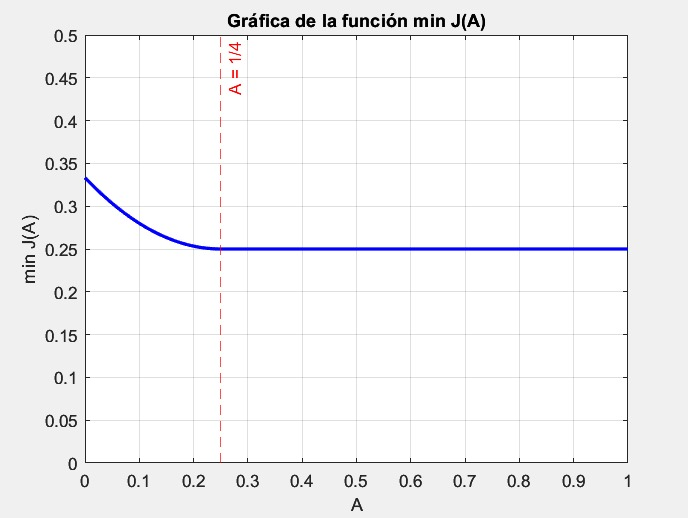
\includegraphics[width=0.5\linewidth]{img/ejercicios/Capitulo-6/ejercicio_6_4_min_j.jpeg}
    \caption{Gráfica función min J(A)}
    \label{ex:6:4:fig:min-j}
\end{figure}


\subsubsection{Resolución 6.5}
% Fuente: Pauta del Auxiliar 10, «KKT — Pregunta 2».
{\color{MidnightBlue}
\begin{enumerate}
  \item[(a)] La unicidad se tiene ya que la función objetivo es estrictamente convexa, para esto basta ver que el hessiano es definido positivo. Notamos que el hessiano es una matriz diagonal donde el término $i$ de la diagonal corresponde a $\alpha_i^2 \beta_i e^{\alpha_i x_i}$, el cual es positivo ya que todas sus componentes son positivas, de esta forma se tiene $\forall z \neq 0, z^T H z = \sum_{i=1}^{n} z_i^2 \alpha_i^2 \beta_i e^{\alpha_i x_i} > 0$ y de esta manera se concluye que el hessiano es definido positivo\footnote{Se puede conlcuir tambien a partir de que sus valores propios son positivos.}.
  \item[(b)] \begin{itemize}
    \item \textbf{Estacionaridad:} $\alpha_i \beta_i e^{\alpha_i x_i} - \mu a_i + \lambda_i - \delta_i = 0 \quad \forall i \in \{1, \ldots, n\}$.
    \item \textbf{Factibilidad primal:} $0 \leq x_i \leq u_i, \quad \sum_{i=1}^{n} a_i x_i \geq b$.
    \item \textbf{Factibilidad dual:} $\mu \geq 0, \lambda_i \geq 0, \delta_i \geq 0 \quad \forall i \in \{1, \ldots, n\}$.
    \item \textbf{Holgura complementaria:} $\mu (b - \sum_{i=1}^{n} a_i x_i) = 0, \quad \lambda_i (x_i - u_i) = 0, \quad -\delta_i x_i = 0$.
\end{itemize}

Para ver que $\mu > 0$, ocupamos la condición de estacionaridad evaluada en algún $x_i > 0$. De esta forma 
\[
\mu = \frac{\alpha_i \beta_i e^{\alpha_i x_i} + \lambda_i}{a_i} > 0.
\]
Donde asumimos que $a_i > 0$ debido a que es el impacto por disminuir $x_i$ unidades las emisiones de la planta $i$, por lo que si fuera negativo es mejor no hacer disminución por lo que esa planta se elimina del problema.
  \item[(c)] Para el desarrollo de esta pregunta hay que notar que existen 3 casos:

\begin{itemize}
    \item Si $x_i \in (0, u_i)$ por holgura complementaria se tiene que $\lambda_i = \delta_i = 0$. De esta manera despejando $x_i$ de la condición de estacionaridad se llega a $x_i = \frac{1}{\alpha_i} \ln \left( \frac{\mu a_i}{\beta_i \alpha_i} \right)$ lo que es consistente con lo pedido.

    \item Si $x_i = 0$ se tiene que $\lambda_i = 0$, en este caso se llega a $x_i = \frac{1}{\alpha_i} \ln \left( \frac{\mu a_i + \delta_i}{\beta_i \alpha_i} \right)$, dada la monotonía del logaritmo (recordar que los multiplicadores son no negativos) se desprende que 
    \[
    x_i = \frac{1}{\alpha_i} \ln \left( \frac{\mu a_i + \delta_i}{\beta_i \alpha_i} \right) = 0 \geq \frac{1}{\alpha_i} \ln \left( \frac{\mu a_i}{\beta_i \alpha_i} \right),
    \]
    de esta manera se trunca hacia arriba $\frac{1}{\alpha_i} \ln \left( \frac{\mu a_i}{\beta_i \alpha_i} \right)$ en 0 para tener la igualdad.

    \item Análogamente si $x_i = u_i$ se tiene $\delta_i = 0$, luego $x_i = \frac{1}{\alpha_i} \ln \left( \frac{\mu a_i - \lambda_i}{\beta_i \alpha_i} \right) = u_i \leq \frac{1}{\alpha_i} \ln \left( \frac{\mu a_i}{\beta_i \alpha_i} \right)$ y nuevamente para tener la igualdad se trunca hacia abajo en $u_i$.
\end{itemize}
  \item[(d)] De la parte b se tiene que en el óptimo $\sum_{i=1}^{n} a_i x_i = b$, sean $I_1, I_2$ e $I_3$ los índices tales que $\frac{\mu a_i}{\beta_i \alpha_i} \leq 1$ ($x_i = 0$) $\ \forall i \in I_1$, $\quad 0 < \frac{1}{\alpha_i} \ln \left( \frac{\mu a_i}{\beta_i \alpha_i} \right) < u_i \quad (x_i = \frac{1}{\alpha_i} \ln \left( \frac{\mu a_i}{\beta_i \alpha_i} \right)) \quad \forall i \in I_2$ y $\quad \frac{1}{\alpha_i} \ln \left( \frac{\mu a_i}{\beta_i \alpha_i} \right) \geq u_i \quad (x_i = u_i) \quad \forall i \in I_3$. Se tiene que 
\[
\sum_{i \in I_2} \frac{a_i}{\alpha_i} \ln \left( \frac{\mu a_i}{\beta_i \alpha_i} \right) = b - \sum_{i \in I_3} a_i u_i,
\]
desde donde se puede obtener $\mu$. Cabe destacar que existe una única solución para $\mu$ dada la unicidad del óptimo $x$.
  \item[(e)] En este caso se debía despejar $\mu$ de la ecuación anterior en función de los parámetros, posteriormente se concluía que $x_i = u$ si $\frac{1}{u} \ln(\mu \gamma) > \alpha_i$, $x_i = \frac{1}{\alpha_i} \ln(\mu \gamma)$ si $\frac{1}{u} \ln(\mu \gamma) \leq \alpha_i$. Notar que el caso $x_i = 0$ se descarta ya que si alguna componente es 0 todas las demás también lo son y no se cumple con la restricción de la calidad del agua.
\end{enumerate}
}


\subsubsection{Resolución 6.6}
% Fuente: Pauta del Control 2, Pregunta 2.
{\color{MidnightBlue}
\begin{enumerate}
  \item[(a)]

Consideramos el problema

\begin{align}
(\bar P)\qquad
\min_{x_1,x_2}\quad
& f_0(x_1,x_2)
=
\frac{1}{2}k_1x_1^2
+
\frac{1}{2}k_2(x_2-x_1)^2
+
\frac{1}{2}k_3(l-x_2)^2
\label{ex:6:6:eq:primal_obj}\\
\text{s.a.}\quad
& \frac{w}{2}-x_1\leq 0,
\label{ex:6:6:eq:R1}\\
& w+x_1-x_2\leq 0,
\label{ex:6:6:eq:R2}\\
& \frac{w}{2}-l+x_2\leq 0,
\label{ex:6:6:eq:R3}
\end{align}

Expandiendo la función objetivo, se obtiene

\begin{align}
f_0(x_1,x_2)
&=
\frac{1}{2}k_1x_1^2
+
\frac{1}{2}k_2\left(x_2^2-2x_1x_2+x_1^2\right)
+
\frac{1}{2}k_3\left(l^2-2lx_2+x_2^2\right)\\
&=
\frac{1}{2}(k_1+k_2)x_1^2
-k_2x_1x_2
+\frac{1}{2}(k_2+k_3)x_2^2
-k_3lx_2
+\frac{1}{2}k_3l^2.
\end{align}

La matriz Hessiana de la función objetivo es

\begin{equation}
\nabla^2 f_0(x_1,x_2)
=
\begin{pmatrix}
k_1+k_2 & -k_2\\
-k_2 & k_2+k_3
\end{pmatrix}.
\end{equation}

Para verificar que esta matriz es definida positiva, se utiliza el criterio de Sylvester. El primer menor principal satisface $k_1+k_2>0,$ mientras que el determinante es

\begin{align}
\det\left(\nabla^2 f_0\right)
&=
(k_1+k_2)(k_2+k_3)-k_2^2=
k_1k_2+k_1k_3+k_2k_3>0.
\end{align}

Por lo tanto, $\nabla^2 f_0(x_1,x_2)\succ 0,$ y, en consecuencia, $f_0(x_1,x_2)$ es estrictamente convexa. Por otra parte, las restricciones pueden escribirse mediante las funciones

\begin{align}
g_1(x_1,x_2)
&=
\frac{w}{2}-x_1,\\
g_2(x_1,x_2)
&=
w+x_1-x_2,\\
g_3(x_1,x_2)
&=
\frac{w}{2}-l+x_2.
\end{align}

Todas estas funciones son afines. Luego, son convexas. Por consiguiente, $(\bar P)$ es un problema de optimización convexo.

Para verificar la condición de Slater, encontremos cotas para $x_1$ y $x_2$. 
Las restricciones estrictas son

\begin{align}
\frac{w}{2}-x_1 &< 0, \label{ex:6:6:eq:slater_r1}\\
w+x_1-x_2 &< 0, \label{ex:6:6:eq:slater_r2}\\
\frac{w}{2}-l+x_2 &< 0. \label{ex:6:6:eq:slater_r3}
\end{align}

De \eqref{ex:6:6:eq:slater_r1} y \eqref{ex:6:6:eq:slater_r3}, se obtiene

\begin{align}
x_1 &> \frac{w}{2}, \label{ex:6:6:eq:x1_lower}\\
x_2 &< l-\frac{w}{2}. \label{ex:6:6:eq:x2_upper}
\end{align}

Además, de \eqref{ex:6:6:eq:slater_r2}, se tiene

\begin{equation}
x_2>x_1+w \Leftrightarrow
x_2-w>x_1.
\end{equation}

Combinando esta última desigualdad con \eqref{ex:6:6:eq:x2_upper}, resulta

\begin{equation}
x_1<x_2-w<l-\frac{3w}{2}.
\end{equation}

Por lo tanto, las cotas para $x_1$ pueden escribirse como

\begin{equation}
\frac{w}{2}<x_1<l-\frac{3w}{2}.
\end{equation}

Tomando el punto medio entre ambas cotas, definimos

\begin{align}
\bar{x}_1
&=
\frac{1}{2}
\left(
\frac{w}{2}
+
l-\frac{3w}{2}
\right)=
\frac{l-w}{2}.
\end{align}

Por otro lado, las cotas para $x_2$ son

\begin{equation}
\bar{x}_1+w<x_2<l-\frac{w}{2}.
\end{equation}

Tomando el punto medio entre estas cotas, se obtiene

\begin{align}
\bar{x}_2
&=
\frac{1}{2}
\left[
\left(
\frac{l-w}{2}+w
\right)
+
\left(
l-\frac{w}{2}
\right)
\right]=
\frac{3l}{4}.
\end{align}

Por tanto, el punto $(\bar{x}_1,\bar{x}_2)
=\left(\frac{l-w}{2},\frac{3l}{4}\right)$ es estrictamente factible. Luego, se cumple la condición de Slater.

  \item[(b)]

Sean $\lambda_1\geq 0$, $\lambda_2\geq 0,$ $\lambda_3\geq 0$ los multiplicadores asociados a las restricciones \eqref{ex:6:6:eq:R1}, \eqref{ex:6:6:eq:R2} y \eqref{ex:6:6:eq:R3}, respectivamente. El Lagrangiano está dado por

\begin{align}
L(x_1,x_2,\lambda_1,\lambda_2,\lambda_3)
&=
\frac{1}{2}k_1x_1^2
+
\frac{1}{2}k_2(x_2-x_1)^2
+
\frac{1}{2}k_3(l-x_2)^2\\
&\quad+
\lambda_1
\left(
\frac{w}{2}-x_1
\right)
+
\lambda_2
\left(
w+x_1-x_2
\right)\\
&\quad+
\lambda_3
\left(
\frac{w}{2}-l+x_2
\right).
\end{align}

La función dual se define como

\begin{equation}
d(\lambda_1,\lambda_2,\lambda_3)
=
\min_{x_1,x_2\in\mathbb{R}}
L(x_1,x_2,\lambda_1,\lambda_2,\lambda_3).
\end{equation}

Por tanto, el problema dual lagrangiano es

\begin{equation}
\max_{\lambda_1,\lambda_2,\lambda_3\geq0}
q(\lambda_1,\lambda_2,\lambda_3) \Leftrightarrow
\max_{\lambda_1,\lambda_2,\lambda_3\geq0}\min_{x_1,x_2\in\mathbb{R}}
L(x_1,x_2,\lambda_1,\lambda_2,\lambda_3)
\end{equation}

Por dualidad débil, se tiene que $d^\star\leq p^\star.$ Sin embargo, dado que el problema primal es convexo y satisface la condición de Slater, se cumple dualidad fuerte: $d^\star=p^\star.$

  \item[(c)]

Las condiciones KKT para este problema son las siguientes.\\

La factibilidad primal exige

\begin{align}
\frac{w}{2}-x_1
&\leq 0,\\
w+x_1-x_2
&\leq 0,\\
\frac{w}{2}-l+x_2
&\leq 0.
\end{align}


La factibilidad dual requiere

\begin{equation}
\lambda_1\geq 0,\qquad
\lambda_2\geq 0,\qquad
\lambda_3\geq 0.
\end{equation}

Las condiciones de holgura complementaria son

\begin{align}
\lambda_1
\left(
\frac{w}{2}-x_1
\right)
&=0,\\
\lambda_2
\left(
w+x_1-x_2
\right)
&=0,\\
\lambda_3
\left(
\frac{w}{2}-l+x_2
\right)
&=0.
\end{align}

La condición de estacionariedad respecto de \(x_1\) y $x_2$ es

\begin{equation}
\frac{\partial L}{\partial x_1}=
k_1x_1+k_2(x_1-x_2)-\lambda_1+\lambda_2=
(k_1+k_2)x_1-k_2x_2-\lambda_1+\lambda_2=0.
\end{equation}

\begin{equation}
\frac{\partial L}{\partial x_2}=
k_2(x_2-x_1)+k_3(x_2-l)-\lambda_2+\lambda_3=
-k_2x_1+(k_2+k_3)x_2-k_3l-\lambda_2+\lambda_3=0.
\end{equation}

Sabemos que un punto \((x_1^\star,x_2^\star)\) es óptimo si existen multiplicadores \((\lambda_1^\star,\lambda_2^\star,\lambda_3^\star)\) que satisfacen la factibilidad primal, factibilidad dual, holgura complementaria y estacionariedad. Puesto que el problema es convexo y satisface Slater, las condiciones KKT son necesarias y suficientes para optimalidad global. Por tanto, es posible encontrar la solución óptima global resolviendo las condiciones KKT. Además, como la función objetivo es estrictamente convexa, la solución óptima primal es única.


  \item[(d)]

Se considera ahora el problema

\begin{align}
\min_{x_1,x_2}\quad
&
\frac{1}{2}x_1^2
+
\frac{1}{2}(x_2-x_1)^2
+
\frac{1}{2}(10-x_2)^2\\
\text{s.a.}\quad
&
1-x_1\leq 0,\\
&
2+x_1-x_2\leq 0,\\
&
x_2-9\leq 0.
\label{ex:6:6:eq:tercera_d}
\end{align}

Se supone que las variables duales asociadas a \((R1)\) y \((R2)\) son nulas: $\lambda_1^\star=\lambda_2^\star=0$. Las ecuaciones de estacionariedad se reducen a

\begin{align}
2x_1-x_2
&=0,\\
-x_1+2x_2-10+\lambda_3
&=0.
\end{align}

De la primera ecuación se obtiene $x_2=2x_1.$ Sustituyendo en la segunda ecuación,

\begin{align}
-x_1+2(2x_1)-10+\lambda_3
&=0,\\
3x_1-10+\lambda_3
&=0,
\end{align}

por lo que $\lambda_3=10-3x_1.$ La condición de holgura complementaria \eqref{ex:6:6:eq:tercera_d} es

\begin{equation}
\lambda_3(x_2-9)=0
\Rightarrow (10-3x_1)(2x_1-9)=0.
\end{equation}

Se analizan los dos casos posibles.

\medskip\noindent\textbf{Caso 1: \(\lambda_3=0\).}

En este caso,

\begin{equation}
10-3x_1=0 \Rightarrow x_1^\star=\frac{10}{3}.
\end{equation}

Por tanto,

\begin{equation}
x_2^\star
=
2x_1^\star
=
\frac{20}{3}.
\end{equation}

Se verifica que este punto es primalmente factible:

\begin{align}
1-x_1^\star
&=
1-\frac{10}{3}
=
-\frac{7}{3}<0,\\
2+x_1^\star-x_2^\star
&=
2+\frac{10}{3}-\frac{20}{3}
=
-\frac{4}{3}<0,\\
x_2^\star-9
&=
\frac{20}{3}-9
=
-\frac{7}{3}<0.
\end{align}

Luego, las tres restricciones tienen holgura estricta y es coherente que $\lambda_1^\star=\lambda_2^\star=\lambda_3^\star
=0.$

\medskip\noindent\textbf{Caso 2: \(x_2=9\).}

Como \(x_2=2x_1\), se tendría $x_1=\frac{9}{2}.$ Sin embargo, verificando factibilidad dual

\begin{equation}
\lambda_3=
10-3\left(\frac{9}{2}\right)=
10-\frac{27}{2}=-\frac{7}{2}<0,
\end{equation}

por lo que $\lambda_3$ no es factible. Por tanto, esta solución debe descartarse.\\

En consecuencia, la solución primal-dual óptima es:

\begin{equation}
\boxed{
x_1^\star=\frac{10}{3},
\quad
x_2^\star=\frac{20}{3}, \quad
\lambda_1^\star
=
\lambda_2^\star
=
\lambda_3^\star
=
0.
}
\end{equation}
\end{enumerate}
}


\subsubsection{Resolución 6.7}
% Fuente: Pauta del Control 2, Pregunta 3, ítems 1–2.
\begin{enumerate}
    \item \textbf{Verdadera.} Sean $f_1,f_2:\mathbb{R}^n\to\mathbb{R}$ funciones convexas y defínase
    \[
        g(x)=\max\{f_1(x),f_2(x)\}.
    \]
    Para cualesquiera $x,y\in\mathbb{R}^n$ y $\lambda\in[0,1]$, por convexidad de $f_1$ y $f_2$ se tiene
    \[
        f_i(\lambda x+(1-\lambda)y)
        \leq \lambda f_i(x)+(1-\lambda)f_i(y),
        \qquad i=1,2.
    \]
    Por tanto,
    \begin{align*}
        g(\lambda x+(1-\lambda)y)
        &=\max_{i\in\{1,2\}} f_i(\lambda x+(1-\lambda)y)\\
        &\leq \max_{i\in\{1,2\}}
        \left\{\lambda f_i(x)+(1-\lambda)f_i(y)\right\}\\
        &\leq \lambda \max_{i\in\{1,2\}} f_i(x)
        +(1-\lambda)\max_{i\in\{1,2\}}f_i(y)\\
        &=\lambda g(x)+(1-\lambda)g(y).
    \end{align*}
    Luego, $g$ es convexa.

    \item \textbf{Verdadera.} Considérese
    \[
        f(x_1,x_2)=x_1^2+5x_2^2-2x_1x_2-10x_1+10x_2.
    \]
    Su matriz Hessiana es
    \[
        \nabla^2 f(x_1,x_2)=
        \begin{pmatrix}
            2 & -2\\
            -2 & 10
        \end{pmatrix}.
    \]
    Como esta matriz es simétrica, basta verificar que es definida positiva. Sus menores principales son
    \[
        2>0,
        \qquad
        \det\begin{pmatrix}
            2 & -2\\
            -2 & 10
        \end{pmatrix}
        =20-4=16>0.
    \]
    Por el criterio de Sylvester, $\nabla^2 f$ es definida positiva. Por tanto, $f$ es estrictamente convexa y, en particular, convexa.
\end{enumerate}



\newpage
\section{Optimización convexa sin restricciones}

\subsection{Algoritmos de optimización continua}

\subsubsection{Descenso por gradiente.}

\subsubsection{Método de Newton.}

\subsection{Ejercicios}

\subsubsection{Ejercicio 7.1}
% Fuente: Control 2, Pregunta 3, ítem 5.
Indique si las siguientes afirmaciones son falsas o verdaderas. En caso de ser verdadera, debe proveer una demostración; en caso contrario, debe dar un contraejemplo.  
\begin{enumerate}
\item Sea $f:\mathbb{R}^{n} \rightarrow \mathbb{R}$ una función convexa y diferenciable que alcanza un único valor mínimo $f(x^{*})$ en $\mathbb{R}^{n}$. Se implementa el algoritmo de descenso de gradiente con tamaño de paso $\alpha > 0$ para resolver el problema $\min_{x \in \mathbb{R}^{n}} f(x)$. Para el caso en estudio, el algoritmo de descenso de gradiente siempre converge a la solución óptima.
\end{enumerate}


\subsection{Resoluciones}

\subsubsection{Resolución 7.1}
% Fuente: Pauta del Control 2, Pregunta 3, ítem 5.
{\color{MidnightBlue}
\begin{enumerate}
    \item \textbf{Falsa.} La convexidad, diferenciabilidad y unicidad del mínimo no garantizan la convergencia del descenso de gradiente para cualquier tamaño de paso fijo $\alpha>0$.

    Considérese la función convexa y diferenciable
    \[
        f(x)=x^2,
        \qquad x\in\mathbb{R}.
    \]
    Esta función tiene un único mínimo global en
    \[
        x^*=0.
    \]
    El método de descenso de gradiente con tamaño de paso fijo $\alpha>0$ genera la sucesión
    \[
        x_{k+1}=x_k-\alpha \nabla f(x_k).
    \]
    Como $\nabla f(x)=2x$, se obtiene
    \[
        x_{k+1}=(1-2\alpha)x_k.
    \]
    Si se toma, por ejemplo, $\alpha=2$ y $x_0\neq 0$, entonces
    \[
        x_{k+1}=-3x_k,
    \]
    de donde
    \[
        x_k=(-3)^k x_0.
    \]
    Esta sucesión no converge a $0$; de hecho, su valor absoluto crece sin límite. Por tanto, no es cierto que el algoritmo converja siempre a la solución óptima para todo $\alpha>0$.
\end{enumerate}
}


\newpage
\section{Tópicos avanzados}

\subsection{Optimización bajo incertidumbre}
\newpage
\input{Secciones/cap9}

\jupyterbutton{https://github.com/paoptlab/Apunte-Optimizacion-A2IC/blob/main/RP-Modelos-Avanzados/Modelos-avanzados.ipynb}


% FIN DEL DOCUMENTO
\end{document}
